%\documentclass[draftdoc]{JSBMLdoc}
\documentclass{JSBMLdoc}

\newcommand{\jsbmlversion}{1.2}
\newcommand{\docdate}{\today}

\makeindex

%%%%%%%%%%%%%%%%%%%%%%%%%%%%%%%%%%%%%%%%%%%%%%%%%%%%%%%%%%%%%%%%%%%%%
% 
% A collection of useful macros that facilitat maintaining the JSBML
% documentation.
%
% Author: Andreas Dr\"ager
%%%%%%%%%%%%%%%%%%%%%%%%%%%%%%%%%%%%%%%%%%%%%%%%%%%%%%%%%%%%%%%%%%%%%

% A
\newcommand{\AbstractNamedSBase}{\texttt{AbstractNamedSBase}\index{SBase@\texttt{SBase}!\texttt{AbstractNamedSBase}}}
\newcommand{\ASTtype}{\texttt{AST\_TYPE\_*}\index{ASTNode@\texttt{ASTNode}!\texttt{AST\_TYPE\_*}}}
\newcommand{\ASTNode}{\texttt{ASTNode}\index{ASTNode@\texttt{ASTNode}}}

% C
\newcommand{\CallableSBase}{\texttt{CallableSBase}\index{JSBML!CallableSBase@\texttt{CallableSBase}}\index{SBase@\texttt{SBase}!CallableSBase@\texttt{CallableSBase}}}
\newcommand{\Compartment}{\texttt{Compartment}\index{SBML!Compartment@\texttt{Compartment}}}

% H
\newcommand{\History}{\texttt{History}\index{annotation!\texttt{History}}}

% K
\newcommand{\KineticLaw}{\texttt{KineticLaw}\index{KineticLaw@\texttt{KineticLaw}}}

% M
\newcommand{\Model}{\texttt{Model}\index{model!Model@\texttt{Model}}}
\newcommand{\ModelCreator}{\texttt{ModelCreator}\index{annotation!\texttt{ModelCreator}}}
\newcommand{\ModelHistory}{\texttt{ModelHistory}\index{annotation!\texttt{ModelHistory}}}

% N
\newcommand{\NamedSBase}{\texttt{NamedSBase}\index{SBase@\texttt{SBase}!\texttt{NamedSBase}}}

% S
\newcommand{\SBase}{\texttt{SBase}\index{SBase@\texttt{SBase}}}
\newcommand{\SBML}{SBML\index{SBML}}
\newcommand{\SBMLDocument}{\texttt{SBMLDocument}\index{SBML!SBMLDocument@\texttt{SBMLDocument}}}
\newcommand{\Serializable}{\texttt{Serializable}\index{Serializable@\texttt{Serializable}}}
\newcommand{\Species}{\texttt{Species}\index{SBML!Species@\texttt{Species}}}

% T
\newcommand{\TreeNode}{\texttt{TreeNode}\index{TreeNode@\texttt{TreeNode}}} 

% U
\newcommand{\UnitDefinition}{\texttt{UnitDefinition}\index{Unit!UnitDefinition@\texttt{UnitDefinition}}}

\hyphenation{
AST-Node
Boo-lean
Cell-De-sig-n-er
Call-able-S-Base
Event-Listener
Event-Hand-l-er
Event-Object
get-Ex-po-nent
get-Ex-po-nent-As-Double
get-Spatial-Di-men-sions
get-Spatial-Di-men-sions-As-Double
J-SB-ML
Ki-ne-tic-Law
lib-SBML-Constants
Lib-SB-ML-Reader
Local-Pa-ra-meter
Plug-in-Action
plug-in
Property-Change-Event
SBML-Document
Tree-Node
Tree-Node-Change-Event
Tree-Node-Change-Listen-er
Tree-Node-With-Change-Support
time-Units
Tree-Node
}


\hypersetup{
  bookmarksopenlevel={1},
  bookmarksnumbered={true},
  breaklinks={true},
  pdfpagemode={UseOutlines},
  pdftitle={User guide for JSBML},
  pdfauthor={Andreas Dr\"ager} {Nicolas Rodriguez} {Alex Thomas} {Marine Dumousseau}
 {Alexander D\"orr} {Clemens Wrzodek} {Finja B\"uchel}
{Florian Mittag} {Nicolas Le Nov{\`e}re} {Andreas Zell} {Michael Hucka},
  pdfsubject={Software guide},
  pdfkeywords={JSBML} {libSBML} {Java} {SBML} {API} {LaTeX} {documentation}
{manual} {guide} {code examples},
  pdfview={FitV},
  pdffitwindow={true},
  pdfstartview={FitV},
  pdfnewwindow={false},
  pdfdisplaydoctitle={true},
  pdfhighlight={/P},
  plainpages={false},
  unicode={true}
}

\definecolor{dkgreen}{rgb}{0,0.6,0}
\definecolor{gray}{rgb}{0.5,0.5,0.5}
\definecolor{mauve}{rgb}{0.58,0,0.82}

\lstset{ %
  language=Java,                  % the language of the code
%  basicstyle=\footnotesize,       % the size of the fonts that are used for the code
  numbers=left,                   % where to put the line-numbers
  numberstyle=\tiny\color{gray},  % the style that is used for the line-numbers
  stepnumber=1,                   % the step between two line-numbers. If it's 1, each line 
                                  % will be numbered
  numbersep=5pt,                  % how far the line-numbers are from the code
  backgroundcolor=\color{white},  % choose the background color. You must add \usepackage{color}
  showspaces=false,               % show spaces adding particular underscores
  showstringspaces=false,         % underline spaces within strings
  showtabs=false,                 % show tabs within strings adding particular underscores
  frame=single,                   % adds a frame around the code
  rulecolor=\color{black},        % if not set, the frame-color may be changed on line-breaks within not-black text (e.g. commens (green here))
  tabsize=4,                      % sets default tabsize to 2 spaces
  captionpos=b,                   % sets the caption-position to bottom
  breaklines=true,                % sets automatic line breaking
  breakatwhitespace=false,        % sets if automatic breaks should only happen at whitespace
  title=\lstname,                 % show the filename of files included with \lstinputlisting;
                                  % also try caption instead of title
  keywordstyle=\color{blue},          % keyword style
  commentstyle=\color{dkgreen},       % comment style
  stringstyle=\color{mauve},         % string literal style
  escapeinside={|}{|},            % if you want to add a comment within your code
  morekeywords={*,...}               % if you want to add more keywords to the set
}

% -----------------------------------------------------------------------------
\begin{document}

\title{\textls[20]{JSBML User Guide}}

\version{\jsbmlversion\\[0.5em]{\normalsize\emph{Document build date: \docdate}}}

\newcommand{\where}[1]{\,\textsuperscript{#1}}
\newcommand{\divider}[1]{\multicolumn{3}{c}{\emph{#1}:}}

\author{%
  \setlength{\tabcolsep}{20pt}%
  \begin{tabular}{@{}ccc@{}}
    \divider{Authors}\\[0.75em]
    Andreas Dr\"ager\where{a}       & Nicolas Rodriguez\where{b,c} & Thomas M. Hamm\where{a}\\
    Alex Thomas\where{d,e}          & Marine Dumousseau\where{c}   & Alexander D\"orr\where{a}\\
    Clemens Wrzodek\where{a,f}      & Finja Wrzodek\where{a,b}     & Florian Mittag\where{a,b}\\
                                    & Michael Hucka\where{g}\\[2em]
    \divider{Principal investigators}\\[0.75em]
    Bernhard \O. Palsson\where{d,e} & Andreas Zell\where{a}        & Nicolas Le Nov\`ere\where{b,c}\\
                                    & Michael Hucka\where{g}\\[2em]
    \divider{Institutional affiliations}\\[0.5em]
  \end{tabular}
  \\
  \begin{normalsize}
  \where{a\,}Center for Bioinformatics Tuebingen, University of Tuebingen, T\"ubingen, Germany
  \\[0.25em]
  \where{b\,}The Babraham Institute, Babraham Campus, Cambridge, UK
  \\[0.25em]
  \where{c\,}European Bioinformatics Institute, Wellcome Trust Genome Campus, Hinxton, Cambridge, UK
  \\[0.25em]
  \where{d\,}Systems Biology Research Group, University of California, San Diego, La Jolla, CA, USA
  \\[.25em]
  \where{e\,}Novo Nordisk Foundation Center for Biosustainability, University of California, San Diego, La Jolla, CA, USA
  \\[0.25em]
  \where{f\,}Roche Pharmaceutical Research and Early Development, pRED Informatics, Roche Innovation Center, Penzberg, Germany
  \\[.25em]
  \where{g\,}Computing and Mathematical Sciences, California Institute of Technology, Pasadena, CA, USA
  \end{normalsize}
}

\frontNotice{SBML (the Systems Biology Markup Language) is an XML-based
  model representation format for storing and exchanging computational
  descriptions of biological processes.  To read, write, manipulate, and
  perform higher-level operations on SBML files and data streams, software
  applications need to map SBML entities to suitable software objects.
  JSBML provides a pure Java library for this purpose.  It supports all
  Levels and Versions of SBML and provides many powerful features,
  including facilities to help migrate from the use of libSBML (a popular
  library for SBML that is not written in Java).
  \\ \\
  This document provides an introduction to JSBML and its use.  It is aimed
  at both developers writing new Java-based applications as well as those
  who want to adapt libSBML-based applications to using JSBML.  This user
  guide is a companion to the JSBML API documentation.
  \\ \\
  \centerline{The JSBML home page is \url{\jsbmlHomePageURL}.}\\
  \centerline{The JSBML discussion group is \url{\jsbmlGroupURL}.}  }


\maketitlepage
\maketableofcontents
\clearpage


\chapter{Getting started with JSBML}
\label{chp:getting-started}

JSBML is a Java\TTra library that will help you to read, write and
manipulate SBML (Systems Biology Markup Language)
files~\cite{Draeger2011a, Draeger2011b}. This chapter provides
information for quickly getting started with using JSBML.

Before you can use JSBML, you will need to obtain a copy of the library.
\sec{sec:obtaining-jsbml} below describes different ways of doing
this, and explains which additional libraries you may need. JSBML also
requires the use of a Java Runtime Environment (JRE) version~1.6 or
later~\cite{JavaDownloadURL}. \index{Java Runtime Environment (JRE)} In the
rest of this document, we assume that you have already installed a suitable
JRE or Java Development Kit (JDK), and know how to configure the Java class
path on your system. \index{Java Development Kit (JDK)}

It is also essential to \emph{understand SBML} in order to be able to use
it (and JSBML) properly. If you are not already familiar with SBML, a good
starting point for learning about it is the latest SBML
specification~\cite{SBMLspecs}. You can find answers to many questions in
the SBML FAQ~\cite{SBMLFAQ} and optionally by asking on one of the SBML
discussion lists~\cite{SBMLforums}.

% -*- TeX-master: "User_guide"; fill-column: 75 -*-

\section{Obtaining and using JSBML}
\label{sec:obtaining-jsbml}

We provide four options for obtaining a copy of JSBML: (1) download the JAR
file distribution for JSBML complete with dependencies, that is, packaged
with third-party Java libraries needed by JSBML; (2) download the JAR file
distribution for JSBML \emph{excluding} dependencies; (3) download the
source code distribution; and (4) obtain the source code directly from the
project's Subversion repository. These four options are described below.


\subsection{The JSBML archive with dependencies}

The version of the archive that includes dependencies is a merged JAR file
that contains all of JSBML's required third-party libraries. You can
download it from the JSBML area on SourceForge~\cite{JSBMLdownload}. Once
you have installed the JAR file on your computer, it is sufficient to add
it to your Java build and/or class path in order to use JSBML.

\subsection{The JSBML archive without dependencies}

\begin{table}[b]
  \caption{List of other, third-party libraries needed by JSBML.}
  \label{tab:dependencies}
  \centering
  \rowcolors{2}{sbmlrowgray}{}
  \renewcommand{\arraystretch}{1.1}
  \begin{tabular}{>{\ttfamily}lp{2.26in}l}
    \toprule
    \textbf{\sffamily Library name} & \textbf{Purpose} & \textbf{Source URL} \\
    \midrule
    biojava-ontology-4.0.0.jar
    & biojava ontology-related classes~\citep{Holland2008}.
    \index{Ontology}
    & \href{http://biojava.org}{biojava.org} \\

    junit-4.8.jar
    & Unit-test support library; only needed if you \mbox{intend} to
    run the tests in the \code{tests} folder.
    & \href{http://www.junit.org}{www.junit.org} \\

    stax2-api-3.1.4.jar
    & Used for reading and writing XML.
    & \href{http://docs.codehaus.org/display/WSTX/StAX2}{docs.codehaus.org/display/WSTX/StAX2} \\

    woodstox-core-5.0.1.jar
    & Used for reading and writing XML.
    & \href{http://woodstox.codehaus.org}{woodstox.codehaus.org} \\
    
    staxmate-2.3.0.jar
    & Used for reading and writing XML. Provides a more user-friendly StAX
    interface.
    & \href{http://staxmate.codehaus.org}{staxmate.codehaus.org} \\

    xstream-1.3.1.jar
    & Used for reading and writing XML, specifically parsing results from
    the SBML validator.
    & \href{http://xstream.codehaus.org}{xstream.codehaus.org} \\

    jigsaw-dateParser.jar
    & Portion of the \emph{Jigsaw} library (version from
    Dec. 2010), containing classes for date manipulation. 
    & \href{http://jigsaw.w3.org}{jigsaw.w3.org} \\

    log4j-1.2-api-2.3.jar 
    & Libraries for logging errors and other diagnostics.
    & \href{http://logging.apache.org/log4j}{logging.apache.org/log4j} and \href{http://www.slf4j.org}{slf4j.org} \\

    log4j-api-2.3.jar \\ log4j-core-2.3.jar \\ log4j-slf4j-impl-2.3.jar \\ slf4j-api-1.7.21.jar \\

    \bottomrule
  \end{tabular}
\end{table}

The version of the JSBML archive that excludes dependencies is a JAR file
that contains only JSBML classes. You can download it from the JSBML area
on SourceForge~\cite{JSBMLdownload}. Since it does not include the
third-party libraries needed by JSBML to operate, you will need to obtain
and download those libraries separately. \tab{tab:dependencies} lists
what they are. Once you have installed the JSBML JAR file \emph{and} these
third-party libraries on your computer, you will need to add them
\emph{all} to your Java build and/or class path in order to use JSBML.


\subsection{Maven dependencies}

JSBML can also be obtained through Apache Maven~\citep{ApacheMaven}.
If you are already using Maven in your project, you can add JSBML
as a dependency, just add the following lines into your pom.xml:

\begin{example}[language=XML, title={Maven instructions to add to your pom.xml.}]
  <repositories>
    <repository>
      <id>ebi-repo</id>
      <name>The EBI repository</name>
      <url>http://www.ebi.ac.uk/~maven/m2repo</url>
      <releases><enabled>true</enabled></releases>
    </repository>
  </repositories>

  <dependencies>
    <dependency>
      <groupId>org.sbml.jsbml</groupId>
      <artifactId>jsbml</artifactId>
      <version>|\jsbmlversion|</version>
    </dependency>
  </dependencies> 
\end{example}

The jsbml artifact will include jsbml-core plus all L3 packages. Like this
there is not need to list all the packages by hand and when
a new one is developed, you will get it without having to make too much change to your
pom files. 

If you want to pick which package to include, you can list them one by one, there are
further instructions at \url{http://sbml.org/Software/JSBML/docs/Maven_Configuration}.


\subsection{The JSBML source archive}
\label{sec:jsbml-source-archive}

The source distribution for JSBML is similar to the JAR distribution that
excludes third-party dependency libraries, except that the JSBML files are
not compiled into class files; you must compile them yourself. As with the
other options described above, the source distribution is available from
the JSBML area on SourceForge~\cite{JSBMLdownload}, as an archive file in
ZIP format.

Download whichever format is more convenient for you and unpack the archive
on your computer somewhere.  The act of unpacking the archive will create a
folder on your computer named after the distribution version; for
example, this may be ``\code{jsbml-}\jsbmlversion''.  Next, you will need to compile
the Java source code.  JSBML comes with a \emph{build file} (i.e., scripted
instructions in a specialized format) for Apache Ant~\citep{ApacheAnt};
you can use other approaches for compiling the JSBML classes and
performing other tasks, but Ant provides an especially convenient approach.
For the rest of the instructions below, we use Ant.  Here is an example of
how to compile the JSBML class files after you have unpacked the source
code archive:

\begin{example}[style=bash, title={Compiling JSBML with Ant; this example
    uses Bash shell syntax.}] 
cd jsbml-|\jsbmlversion|
ant compile
\end{example}

Next, if you wish to run the self-tests included with JSBML, you can do so by
running the following command:

\begin{example}[style=bash, title={Running the unit tests provided with JSBML.}]
ant test
\end{example}

Finally, if you want to produce a JAR file containing all the JSBML
compiled class files, run the following command:

\begin{example}[style=bash, title={Creating a JAR file.}]
ant jar
\end{example}



\subsection{The JSBML source code repository}
\label{sec:SourceDistribution}

The fourth approach to obtaining a copy of JSBML is to retrieve it directly
from the Subversion repository~\cite{JSBMLSVN}.  Here is an example of how
to retrieve the latest version of the JSBML sources:

\newcommand{\dirname}{\code{\emph{\color{winered}jsbml}}\xspace}

\begin{example}[style=bash, title={Downloading the latest JSBML 
    sources from the JSBML project's Subversion repository.}]
svn co https://svn.code.sf.net/p/jsbml/code/trunk |\dirname|
cd |\dirname|
\end{example}

(The name you give to the copy on your computer is up to you.  We used
``\dirname'' in this example, but you could name the folder something else
if you wish.)  Once you have retrieved the folder from the Subversion
repository, you can compile the source files and create a JAR file.  Please
refer to the instructions in \sec{sec:jsbml-source-archive}.

The Subversion repository contains copies of all the third-party libraries
listed in \tab{tab:dependencies} and needed by JSBML.  They are
located in the folder ``\dirname''\code{/core/lib}.


\subsection{Setting up Eclipse}
\label{sec:SettingUpEclipse}

To set up Eclipse to work with JSBML, first add the \texttt{src},
\texttt{test} and \texttt{resources} folder of the JSBML distribution to your
Eclipse build path, and add all of the \texttt{.jar} files found in the
\texttt{lib} folder.

Next, you need to do an extra step to configure the annotation processor,
because the different parsers in JSBML are registered automatically using
Java annotations.  To configure the annotation processor in Eclipse, follow
the instructions found on the web page
\url{https://github.com/niko-rodrigue/spi/blob/wiki/EclipseSettings.md}.
 The jar file of the annotation processor is located in the jsbml source tree at
 ``\dirname''\code{/core/lib/spi-full-0.2.4.jar}. If you checkout 
the full trunk (and not just the core), you can find a folder dev, which 
contains a README.txt file that has also these instructions and further 
important information.

Finally, you can run the \code{ParserManager} class to check that the list of
parsers are not empty and that they contain the parsers you need.


\subsection{Optional extensions, modules and examples available for JSBML}
\label{sec:dependencies}

JSBML provides a number of additional extensions, modules and example
programs that you may find useful in your work.  The \emph{extensions} are
optional add-ons that implement support for SBML Level~3 Packages; these
packages extend SBML syntax to support, for example, storing the layout of
a model's graphical diagram directly in the SBML file.  The JSBML
\emph{modules} provide additional features and interfaces, for example, to
allow CellDesigner~\cite{Funahashi2003} plugins to use JSBML.  Finally, the
JSBML \emph{examples} are full-fledged applications that demonstrate the
use of JSBML in actual running software.  Each of these optional components
of JSBML is available from the project's code repository (and in some
cases, from the download area on SourceForge~\cite{JSBMLdownload}).  In the
subsections below, we explain how to obtain copies of them from the
repository.


\subsubsection{JSBML Extensions}

The JSBML repository's \code{extensions} folder contains a separate
subfolder for each currently-implemented JSBML extension. You can either
retrieve a copy of each extension separately, or obtain the complete
\code{extensions} portion of the repository.  Here we explain the latter.

First, find a suitable location on your computer where you would like to
place the JSBML extensions folder.  (We suggest placing it side-by-side at
the same level as your JSBML core folder, e.g., next to the folder
``\dirname'' discussed above.)  Then, perform the following step:

\begin{example}[style=bash, title={Downloading the latest JSBML extensions
    source folder from the project's Subversion repository.}] 
svn co https://svn.code.sf.net/p/jsbml/code/trunk/extensions jsbml-extensions
\end{example}

Each of the extensions has its own Ant build script, located in a file
named (as per Ant conventions) ``\code{build.xml}'' within the extension's
subfolder.  To build, for example, the \code{layout} extension, you could
do the following:

\begin{example}[style=bash, title={Compiling the ``\code{layout}'' extension.}]
cd extensions/layout
ant compile
\end{example}


\subsubsection{JSBML Modules}
\label{sec:jsbml-modules}

JSBML currently provides six additional modules.  Each provides features
for task-specific purposes. Binary versions of the modules can be found at
the download site of JSBML~\cite{JSBMLdownload}; here we explain how you
can obtain the most recent versions of the modules directly from the source
code repository.  (Note: at the time of this writing, only the
\code{tidy}, \code{CellDesigner} and the \code{libSBMLio} module have been extensively
tested.)

First, find a suitable location on your computer where you would like to
place the JSBML modules folder.  We suggest creating a folder named
``\code{modules}'' placed side-by-side at the same level as your JSBML core
folder, e.g., next to the folder ``\dirname'' discussed above.

\begin{example}[style=bash, title={Creating a folder for the modules.}]
mkdir modules
cd modules
\end{example}

\newcommand{\modulename}{\code{\emph{\color{winered}modulename}}\xspace}

Next, perform the following operation, once for each of the modules you
would like to obtain, where the variable \modulename is one of the names
listed in the first column of \tab{tab:jsbml-modules}:

\begin{example}[style=bash, title={Obtaining a JSBML module.}]
svn co https://svn.code.sf.net/p/jsbml/code/trunk/modules/|\modulename| |\modulename|
\end{example}

(In other words, if you would like to obtain both the Android and libSBMLio
modules, execute the command above twice, once with \code{android} in place
of \modulename and a second time with \code{libSBMLio} in place of
\modulename.)  Once they're downloaded, please check inside each module
directory for information about how to use them.

\begin{table}[thb]
  \caption{JSBML modules available today.}
  \label{tab:jsbml-modules}
  \centering
  \rowcolors{2}{sbmlrowgray}{}
  \begin{tabular}{>{\ttfamily}lp{5.25in}}
    \toprule
    \textbf{\sffamily Module name} & \textbf{Purpose} \\
    \midrule
    android
    & Support for writing JSBML-based programs for Android OS.
    \\
    celldesigner
    & A bridge module that supports writing JSBML-based
    plugins for CellDesigner~\cite{Funahashi2003}
    \\
    compare
    & Facilities for doing comparisons between libSBML and JSBML
    \\
    libSBMLcompat
    & A module that allows easier switching between libSBML and JSBML by
    providing wrapper classes replicating much of libSBML's API in JSBML (in development)
    \\
    libSBMLio
    & A libSBML communications layer.
    \\
    tidy
    & A warper around the SBMLWriter class that use the jtidy library~\cite{jtidy} (a Java port of HTML Tidy) to
    format properly the resulting XML.
    \\
    \bottomrule
  \end{tabular}
\end{table}

You can find more information and explanation about JSBML's modules in \sec{sec:jsbml-modules-details}.


\subsubsection{JSBML Examples}
\label{sec:jsbml-repo-examples}

The JSBML repository's \code{examples} folder contains a separate
subfolder for each sample application.  To obtain them, first, find a
suitable location on your computer where you would like to place the JSBML
examples folder.  We suggest creating a folder named ``\code{examples}''
placed side-by-side at the same level as your JSBML core folder.

\begin{example}[style=bash, title={Creating a folder for the examples.}]
mkdir examples
cd examples
\end{example}

Next, retrieve the examples you would like to obtain.  At the time of this
writing, there is only one example available:

\begin{example}[style=bash, title={Retrieving the \emph{SBML Bar Graph}
    example application.}] 
svn co https://svn.code.sf.net/p/jsbml/code/trunk/examples/sbmlbargraph sbmlbargraph
\end{example}

Finally, please read the ``\code{README.txt}'' file in the freshly-obtained
\code{sbmlbargraph} folder to learn more about how to get started with the
example application.



% -*- TeX-master: "User_guide"; fill-column: 75 -*-

\section[Writing your first JSBML application]{\emph{Hello World}: writing your first JSBML applications}
\label{sec:hello-world}

In this section, we present two examples of using JSBML. The first is a
program that reads a file containing an SBML document and displays its
components in a Java \JTree graphical object. The second example
illustrates the creation of an object representing an SBML document (which,
in JSBML, is represented programmatically using an object of class
\SBMLDocument), as well as writing that object to a file. These basic
examples should help serve as a foundation for writing your own, more
elaborate programs.


\subsection{Reading and visualizing an \codeNC{SBMLDocument} object}

\fig{fig:JSBMLvisualizer-source} shows the listing of a simple program
called ``\code{JSBMLvisualizer}''.  The source is included in the JSBML
distribution, in the ``\texttt{doc/user\_guide/src}'' subdirectory.  As
with most simple JSBML-based programs, to compile and execute
``\code{JSBMLvisualizer}'', you would execute the following sequence of
commands:

\newcommand{\classpath}{\code{\emph{\color{winered}classpath}}\xspace}

\begin{example}[style=bash, title={Compiling and executing the example program.}]
  javac -classpath |\classpath|JSBMLvisualizer.java
  java -classpath |\classpath|JSBMLvisualizer
\end{example}

\begin{wrapfigure}[24]{r}{2.55in}
  \centering
  \vspace*{-1.8em}
  \setlength{\captionmargin}{1.8em}
  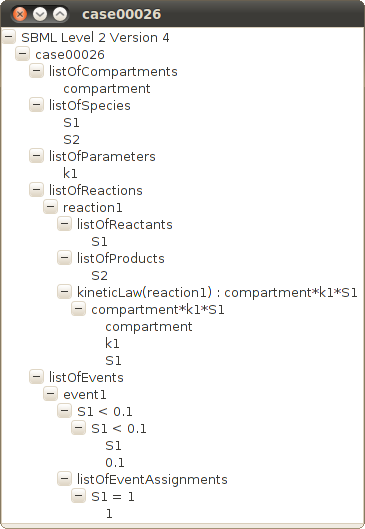
\includegraphics[width=.32\textwidth]{%
    ../posters/2010_ICSB_and_COMBINE/JSBMLvisualizerTransparent.png}
  \caption[Tree representation of an SBML file]{Tree representation of
    the contents of the SBML test file ``\code{case00026}.xml''. In JSBML,
    the hierarchically structured \SBMLDocument can be traversed
    recursively because all instances of \SBase, the parent class,
    implement the interface \TreeNode.}
  \label{fig:JSBMLvisualizer-output}
\end{wrapfigure}
In the example commands above, replace the placeholder text \classpath with
the actual Java class path for the JSBML libraries and its dependencies on
your particular computer; we do not show an exact value here because it
depends on where you have installed the JAR files for JSBML and the
third-party libraries.

When run, the program expects to be given the pathname of a valid SBML
file as \index{SBML!XML file} its sole argument. It uses the static method
\code{read()} defined by the JSBML object class \SBMLReader to read the
file; \SBMLReader returns an object of class \SBMLDocument, the main SBML
document container in JSBML.  Next, the program constructs a new
\code{JSBMLvisualizer} object, which is derived from the standard Java
\JFrame class. It invokes the class constructor (line 9) with the
identifier of the model in the SBML file, obtained by calling
\code{getModel().getId()} on the \SBMLDocument object; this sets the
\JFrame's title to the identifier of the model.  Since JSBML's \SBase
object (and all objects derived from it) implement the \TreeNode interface,
it is possible to create a \JTree directly from the information in an
\SBMLDocument object instance.  (To keep our examples short and focused on
the essentials of using JSBML, we have omitted error checking steps.  A
real application program should guard against various situations, such as
\code{getModel()} or \code{getId()} returning \code{null}, and take steps
to deal with them appropriately. You might also like to read SBML files in
a separate thread and monitor the progress of reading the file in some
progress bar.)

\begin{figure}[ht]
  \exampleFile[style=java, firstline=35, caption={}]{src/org/sbml/jsbml/gui/JSBMLvisualizer.java}
  \caption{Parsing and visualizing the content of an SBML file.}
  \vspace*{-1.5em}
  \label{fig:JSBMLvisualizer-source}
  \index{graphical user interface!\code{JFrame}}
\end{figure}


\fig{fig:JSBMLvisualizer-output} shows the example output when
applying the program to an SBML test model. \index{SBML!test cases} Each
element in the model shows up as an item in the hierarchy displayed by the
Java \JTree object. In the working application, the user can click on the
control boxes (i.e., the boxed ``+'' and ``-'' symbols next to the element
names) to collapse or expand the views of the substructures of an SBML
model.

We hasten to add that this simple program lacks many features that a proper
application should possess.  We kept this example purposefully as simple as
possible so that it is easier to focus on the main point of the example
(which is, how to read an SBML file).  Perhaps the most important missing
aspect is checking for and handling errors that may be encountered when
trying to read and parse the file given as argument to the program.  Not
all SBML files are valid, owing to the unfortunate reality that \emph{not
  all software tools in the world produce syntactically and semantically
  correct SBML}. The JSBML library is flexible and attempts to carry on in
the face of problems, because it is the responsibility of the calling
application to decide when and how problems should be handled. A realistic
application should be coded defensively: it should be prepared for the
possibility of receiving badly-formed input, check for any warnings and
errors reported by \SBMLReader when it attempts to read the SBML file, and
deal with them appropriately. Elsewhere in this document, we provide
examples of checking for errors.

Reading a file is nice, but what about writing an SBML file?  That is the
topic of the next example.

% FIXME tell people where to find the source code to the examples.


\subsection{Creating and writing an \codeNC{SBMLDocument} object}

Our next example, shown in \fig{fig:JSBMLexample-source},
illustrates how to construct an in-memory representation of an SBML model
and write it to a file. The program first creates an \SBMLDocument object,
then attaches a \Model object to it, and then to the \Model adds one
\Compartment, two \Species, and one \Reaction objects. To write the
contents to a file named ``\code{test.xml}'', the program uses a static
method on the JSBML class \SBMLWriter. 

This program also illustrates the preferred approach to the creation of JSBML object instances. 
The only constructor you should need to use is the constructor of the \SBMLDocument, specifying
the SBML Level and Version you want to use. Each JSBML class should have  
\code{create\emph{XYZ}} methods, where \code{\emph{XYZ}} is the subclass name. 
For example, you may have \code{model.createSpecies(String)}, \code{model.createReaction(String)}
or \code{reaction.createReactant()}. These methods will guarantee that callers create a proper
representation of the SBML model.  

\begin{figure}[bht]
  \vspace*{-1ex}
  \exampleFile[style=java, caption={}, firstline=32]{src/org/sbml/jsbml/demo/JSBMLexample.java}
  \vspace*{-1ex}
  \caption{An example of Creating a new \code{SBMLDocument} object and
    writing its content into a file.  (This file is available as
    ``\texttt{doc/user\_guide/src/org/sbml/jsbml/demo/JSBMLexample.java}''
    in the JSBML distribution.)}
  \label{fig:JSBMLexample-source}
  \vspace*{-1em}
\end{figure}

% -*- TeX-master: "User_guide"; fill-column: 75 -*-

\section{More examples}

\fig{lst:LibSBMLio} illustrates the conversion of libSBML data structures
into JSBML data objects. \fig{lst:PluginAction} demonstrates the
implementation of CellDesigner's abstract class \code{PluginAction} and
Listing~\fig{lst:Plugin1} gives a complete example for writing CellDesigner plugins
with JSBML.  \index{CellDesigner} More detailed explanations of JSBML's
modules can be found in \sec*{sec:jsbml-modules-details}, and more complex
examples of using JSBML are available from the JSBML SourceForge repository.
(Please see \sec{sec:jsbml-repo-examples} for information about how to obtain
them.)



\chapter{Differences between JSBML and libSBML}
\label{chp:jsbml-libsbml-diffs}

Prior to the availability of JSBML, the most widely-used API library for
SBML offering a Java interface has been libSBML~\cite{Bornstein2008}. As a
result, many Java application developers working with SBML are already
accustomed to the classes, methods and general approach provided by
libSBML. This chapter discusses the main differences between these two
libraries, and is aimed at current libSBML users who want to transition to
using JSBML. We also provide some programming examples and hints for how
to use and work with JSBML. In addition, we provide an overview of the type hierarchy 
and API of JSBML.

% -*- TeX-master: "User_guide"; fill-column: 75 -*-

\section{Why are there differences?}
\label{sec:jsbml-design-goals}

In developing a pure Java Application Programming Interface (API) for
working with SBML, our intention was not to simply reimplement the Java API
already provided by libSBML~\citep{Bornstein2008}.
\index{application programming interface!libSBML}
We took the opportunity to rethink the API
\index{application programming interface!JSBML} from the ground up to
produce something more natural for Java programmers; moreover, we
benefited from being able to take a fresh look at today's entire set of
SBML specifications~\citep{Hucka2003, Hucka2008, Hucka2010a}
\index{SBML!specification} and redesign, for example, JSBML's type
hierarchy without the constraints of backwards compatibility that libSBML
faces. 

JSBML has also been developed as a library that provides more than only
facilities for reading, manipulating, and writing SBML files and data
streams. Although SBML only defines the structure of representations of
biological processes in files and does not prescribe how its components
should be stored \emph{in computer memory}, many software developers
nevertheless find it convenient to follow similar representational
structures in their programs. \index{model!storage and exchange} With this
in mind, we designed JSBML with the intention that it be directly usable as
a flexible internal data structure for numerical computation,
visualization, and more. With the help of its \emph{modules}, JSBML can
also be used as a communication layer between applications. For instance,
JSBML facilitates the implementation of plugins for
CellDesigner~\citep{Funahashi2003}, \index{CellDesigner} a popular software
application for modeling and simulation in systems biology. Finally, JSBML
(like libSBML before it) hides some of the differences and inconsistencies
in SBML \index{SBML!differences between Levels} that grew into the language
over the years as it evolved from Level to Level and Version to Version;
this makes it considerably easier for developers to support multiple
Levels/Versions of SBML transparently.

Where possible, we maintained many of libSBML's naming conventions for
methods and variables. Owing to the very different backgrounds of the two
libraries, and the fact that libSBML is implemented in C \index{C} and
C++ \index{C++}, some differences are unavoidable. To help libSBML
developers transition more easily to using JSBML, we provide a
compatibility module that implements many libSBML methods as adaptors
around the corresponding JSBML methods.

% FIXME add back somehow:
% during
% the evolution of SBML some elements or properties of elements have become
% obsolete.
% \index{deprecation}%

% -*- TeX-master: "User_guide"; fill-column: 75 -*-

\section{Differences between the class hierarchies}
\label{sec:extended-type-hierarchy}

\begin{sidewaysfigure}[p]
  \centering
  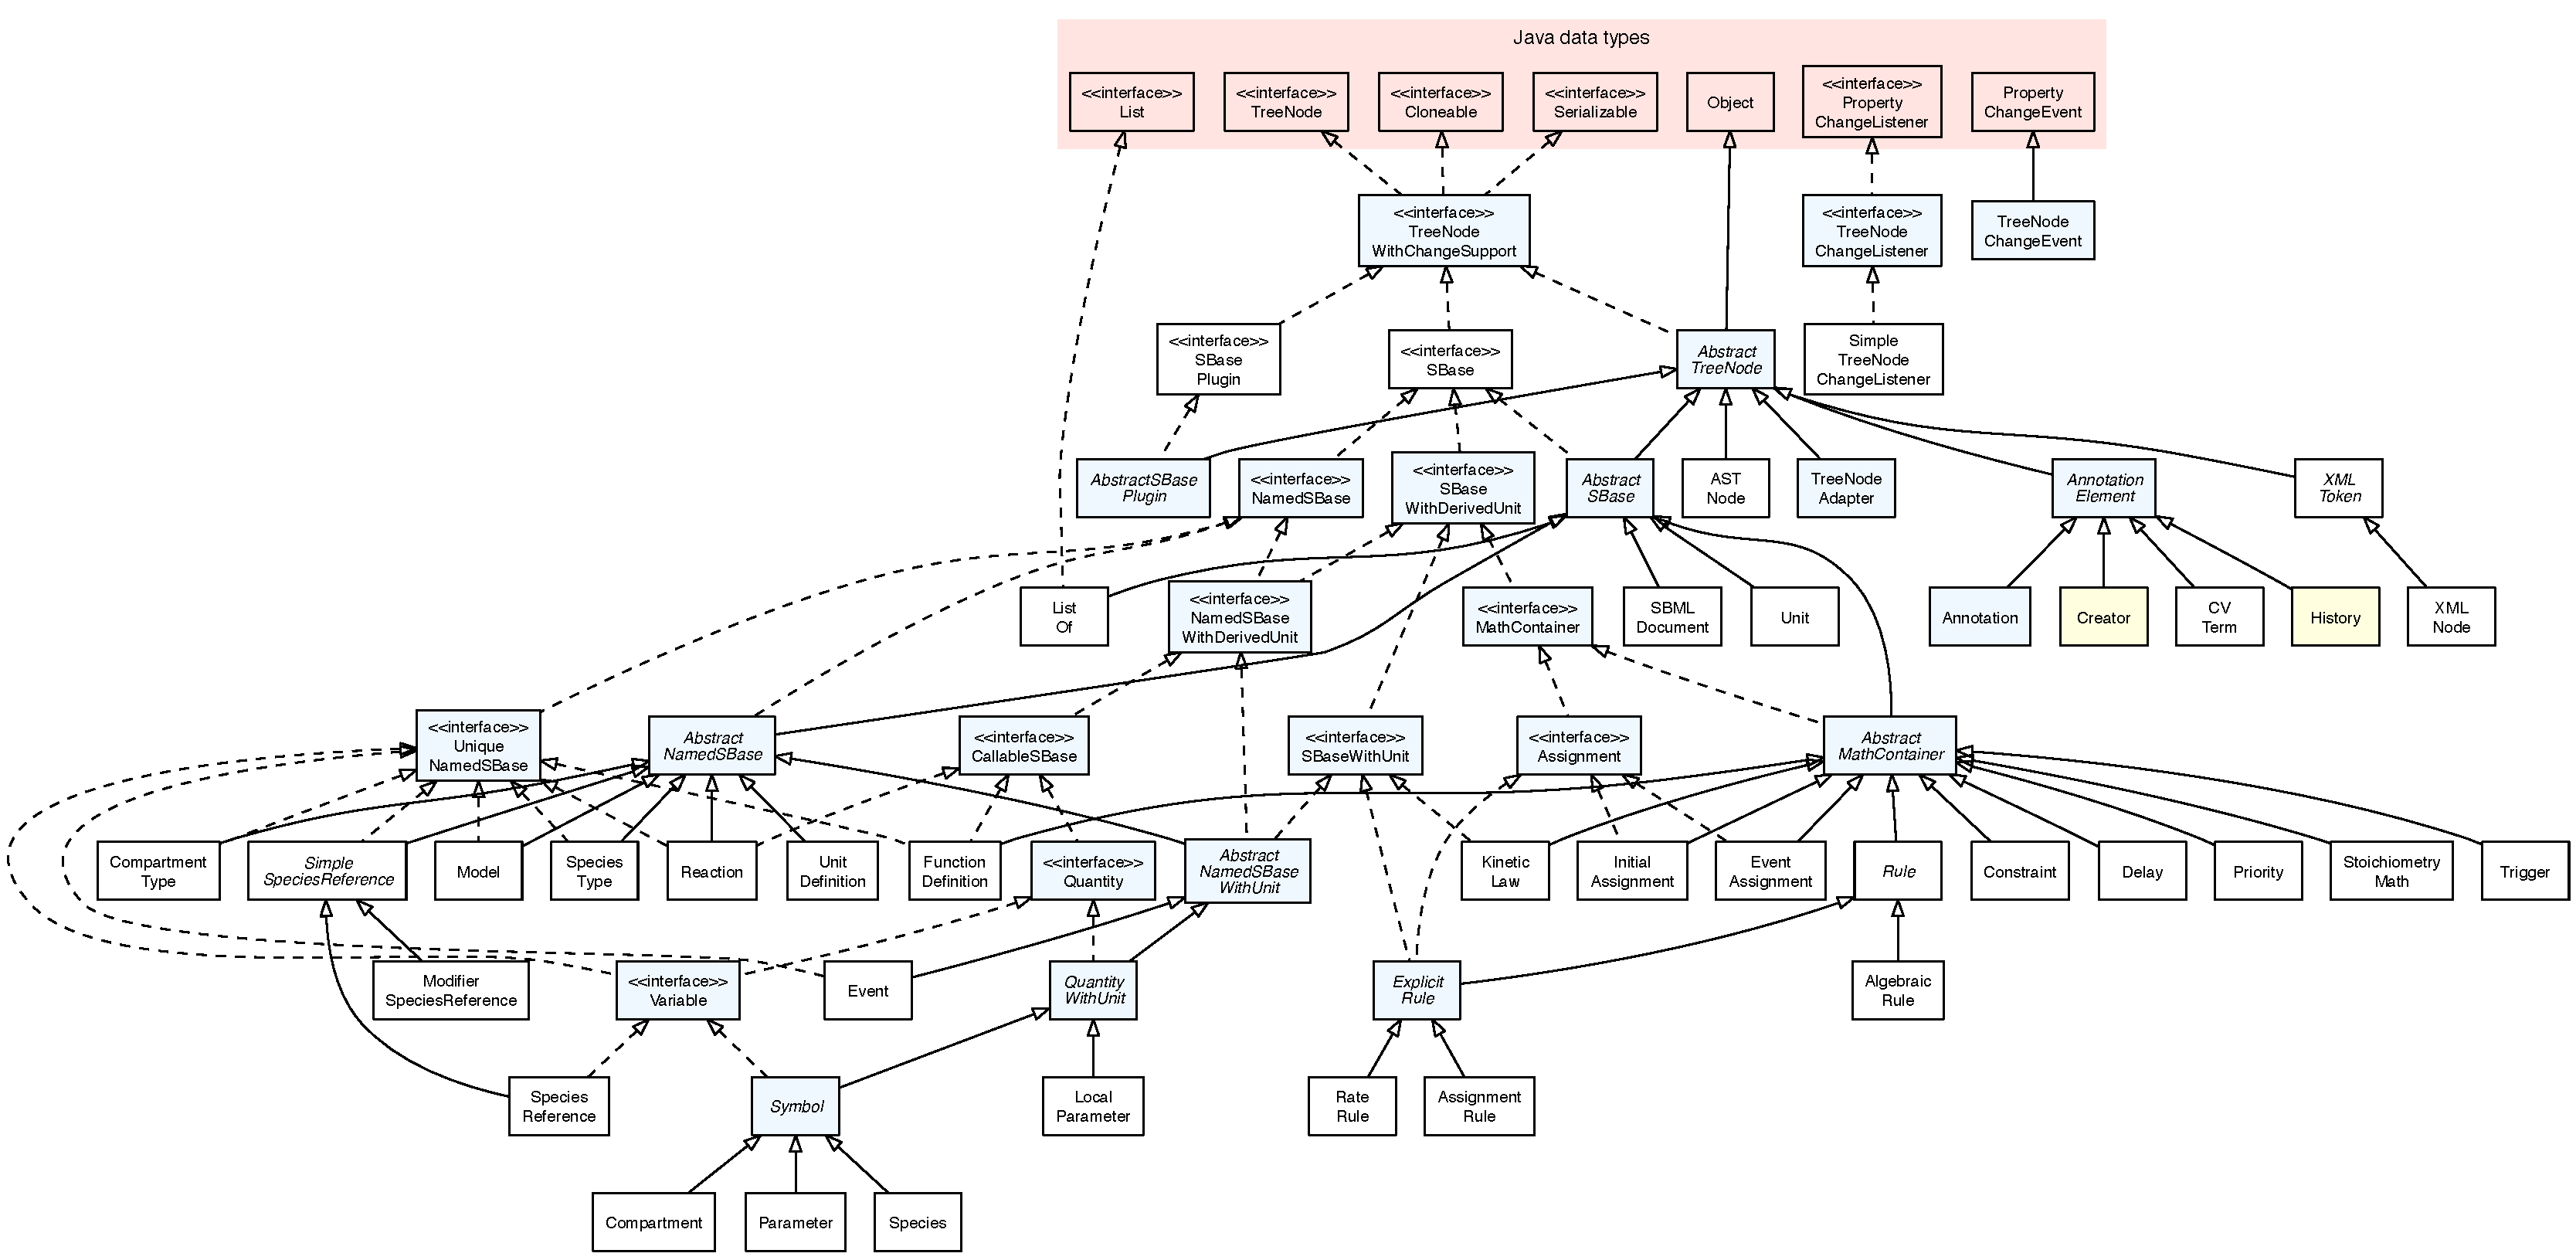
\includegraphics[width=0.97\textwidth]{../common/img/FullTypeHierarchy.pdf}
  \caption[The type hierarchy of the main SBML constructs in JSBML]{The
    type hierarchy of the main SBML constructs in JSBML. The elements
    colored in yellow, \code{Creator} and \code{History}, correspond to
    \code{ModelCreator} and \code{ModelHistory} in libSBML. Elements
    colored in blue are additional, in most cases abstract, data types in
    JSBML that do not have corresponding features in libSBML. Many other
    classes and interfaces in this diagram have no equivalent in libSBML,
    but offer more powerful capabilities for Java programmers. By making
    \SBase extend the interface \TreeNodeWithChangeSupport (another class
    defined by JSBML), which in turn extends the Java interfaces
    \code{Cloneable}, \code{Serializable}, and \TreeNode. All subclasses
    of \code{SBase} also provide the functionality of these classes and
    interfaces. In JSBML, even SBML components that are not defined by
    SBML as actually being derived from \code{SBase} are nevertheless
    derived from \TreeNodeWithChangeSupport; thus, they (and all their
    subclasses) share many common methods and attributes, which makes them
    easy to use when wherever instances of \TreeNode or operations across
    hierarchies of objects are needed. In order to support SBML Level~3
    packages, JSBML version 1.0 adds the interface \SBasePlugin and its
    abstract implementation \AbstractSBasePlugin (shown marked
    with a red border in this diagram).} 
  \label{fig:TypeHierarchy}
\end{sidewaysfigure}

Wherever multiple SBML elements defined in at least one SBML Level/Version
combination \index{SBML!specification} share attributes, JSBML
\index{JSBML!type hierarchy} provides a common superclass, or at least a
common interface, that gathers methods for manipulating the shared
properties. Consequently, JSBML's type hierarchy
\index{application programming interface!JSBML} is richer than libSBML's (see
\vrefrange{fig:TypeHierarchy}{fig:MathContainerHierarchy}).

Just as in libSBML, \index{application programming interface!libSBML} all
SBML objects derived from SBML's \SBase extend the JSBML abstract class
\SBase, but in JSBML, \SBase is an interface rather than an object class.
This allows more complex relations to be defined between derived data
types. In contrast to libSBML, JSBML's \SBase extends the interface
\TreeNodeWithChangeSupport, which in turn extends three other interfaces:
\Cloneable, \Serializable, and \TreeNode (\fig*{fig:SBase}).
This brings with it various advantages. One is that, because all elements
defined in JSBML \index{cloning} override the \code{clone()} method from
the class \code{java.lang.Object}, \index{Object@\code{Object}} all JSBML
elements can be deeply copied and are therefore \emph{cloneable}. Further,
extending the interface \Serializable makes it possible for JSBML
\index{application programming interface!JSBML} objects to be stored in
binary form without having to write them explicitly to an SBML file.
\index{SBML!XML file} In this way, programs can easily load and save their
in-memory objects or send data structures across a network connection
without the need of additional file encoding and subsequent parsing.

The third interface extended by \SBase, \TreeNode is defined in Java's
\emph{Swing} \index{graphical user interface!Swing} package; however,
\TreeNode is actually independent of any graphical information.  (We hasten
to add that JSBML does \emph{not} depend on any particular graphical user
interface, and no other classes are initialized when loading \TreeNode from
Java Swing.)  \TreeNode defines recursive methods on hierarchically
structured data types, such as iteration over all successors. This means
that, if a developer so desires, all instances of JSBML's \SBase interface
can be passed directly to the Java Swing \index{graphical user
  interface!Swing} class \JTree \index{graphical user
  interface!\code{JTree}} for easy visualization. The program shown in
\fig{fig:JSBMLvisualizer-source} (and whose output is presented in
\fig{fig:JSBMLvisualizer-output}) demonstrates the simple code
needed to parse an SBML file \index{SBML!XML file} and immediately display
its contents in a \JFrame. \index{graphical user interface!\code{JFrame}}
The \ASTNode class in JSBML is also derived from all these three interfaces
and can hence be cloned, serialized, and visualized in the same way.

\begin{figure}[hb]
 \centering
 \vspace*{2ex}
 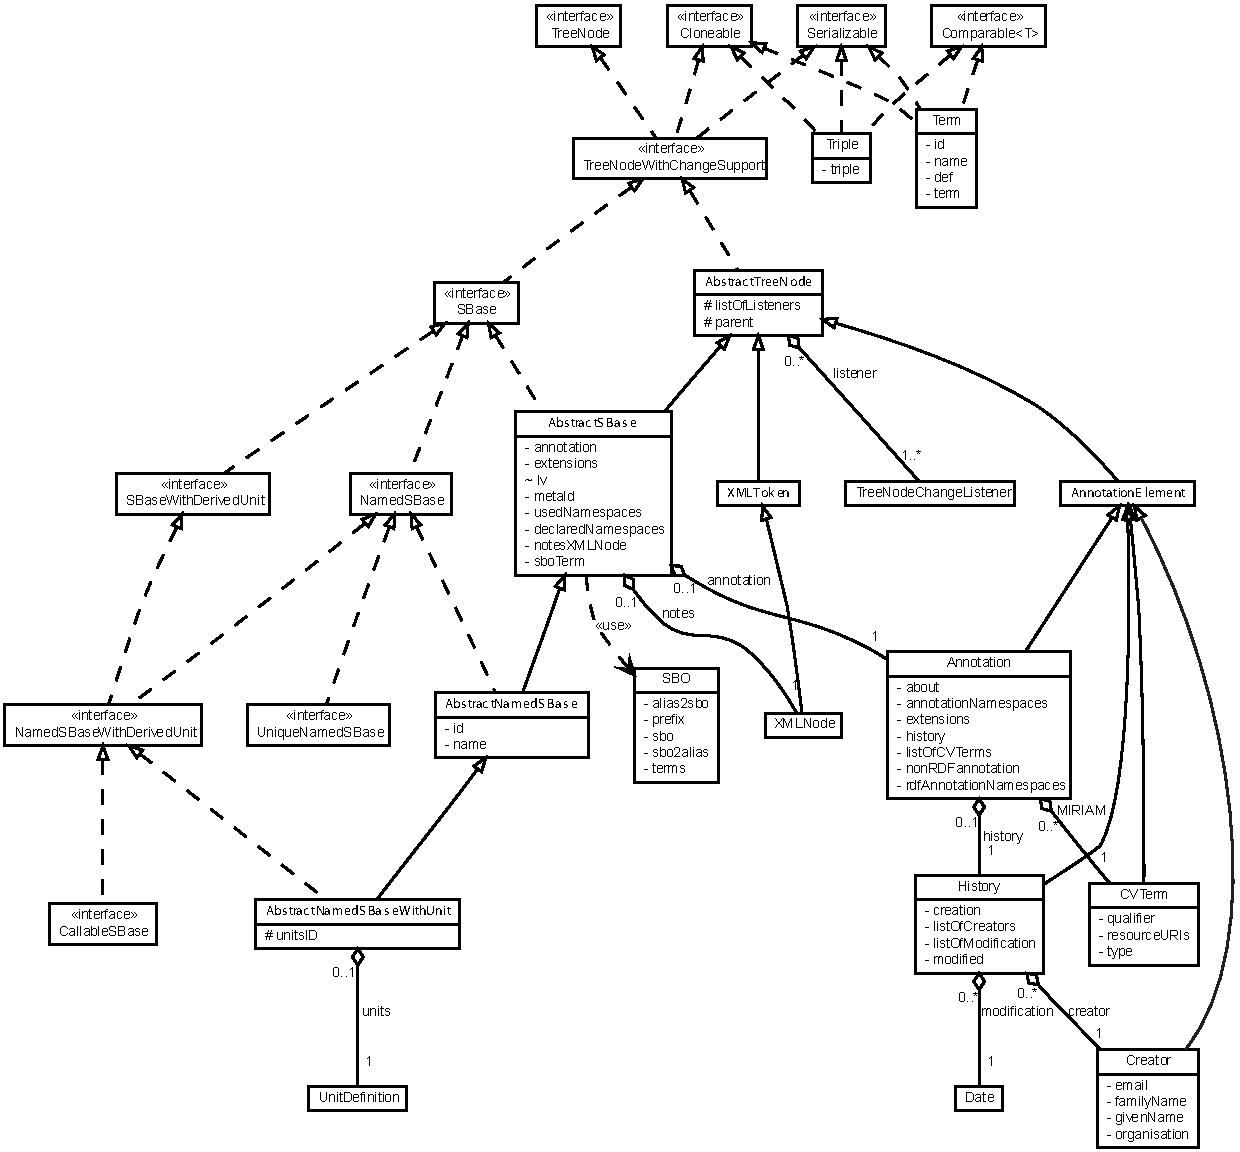
\includegraphics[width=\textwidth]{../common/img/SBase.pdf}
 % SBase.pdf: 1001x568 pixel, 72dpi, 35.31x20.04 cm, bb=0 0 1001 568
 \caption[The interface \code{SBase}]{The interface \SBase. This figure
   shows the most important top-level data structures in JSBML, with a
   focus on the differences compared to libSBML. For the sake of clarity,
   we have omitted all the methods on the classes shown here. As can be
   seen in this diagram, all data types that
   represent SBML constructs in JSBML extend \AbstractTreeNode.
   Derivatives of \SBase extend either one of the two abstract
   classes \AbstractSBase or \AbstractNamedSBase, which in turn
   also extend \AbstractTreeNode. The class \SBO implements
   facilities for parsing the ontology\index{Ontology} file provided on the
   SBO web site (\url{http://www.ebi.ac.uk/sbo/main/}) in OBO format (Open
   Biomedical Ontologies), using a parser provided by the BioJava
   project~\citep{Holland2008}. \SBO stores its ontology in
   the classes \code{Term} that are interrelated in \code{Triples}
   consisting of subject, predicate, and object (each being an instance of
   \code{Term}).}
 \label{fig:SBase}
\end{figure}


\subsection{Common interface for hierarchical structures: \codeNC{AbstractTreeNode}}%
\label{sec:AbstractTreeNode}
\index{TreeNode!AbstractTreeNode@\code{AbstractTreeNode}}

When reading the SBML specifications~\citep{Hucka2003, Hucka2008,
  Hucka2010a}, \index{SBML!specification} it quickly becomes apparent that
an SBML model has a tree-shaped, hierarchical structure, with \SBase being
the superclass of nearly all other SBML components. In JSBML, other kinds of
objects besides \SBase are also organized hierarchically within an
\SBMLDocument.  To unify the programming interfaces for all of these kinds
of objects, JSBML defines abstract data types as top-level ancestors for
its \SBase implementation as well as all other hierarchical elements, such
as \Annotation, \ASTNode, \Creator, \CVTerm, \History, and \XMLNode (for
notes in XHTML \index{XHTML} format).

As mentioned above, the interface \TreeNodeWithChangeSupport defines a
cloneable and serializable version of \TreeNode. (See the diagram in
\fig{fig:SBase}.) In addition, it also provides methods to notify
dedicated \TreeNodeChangeListener class objects about any changes within
the data structure. Its abstract implementation, \AbstractTreeNode,
implements many of the methods inherited from \TreeNodeWithChangeSupport
and also maintains a list of change listeners (implemented as
\TreeNodeChangeListener{}s). Furthermore, this class contains a basic
implementation of the methods \code{equals} and \code{hashCode}, which both
make use of a recursive call over all descendants within the hierarchical
SBML data structure. By basing the object definitions on this class, the
implementation of all derived classes has become much simpler.


\subsection{Common root of SBML components: \codeNC{AbstractSBase}}

With \SBase being an interface rather than an object class, most SBML-related
object classes in JSBML extend the abstract implementation \AbstractSBase, as
shown in \fig{fig:SBase}.  One of the features of this abstract class is
that it tracks the SBML Level and Version of every concrete object
implementing it.  The need for tracking each object's Level+Version
combination individually (a feature shared with libSBML) may seem odd at
first.  The need arises because a software system may need to work with more
than one combination at a given time; it may also need to create individual
SBML components before they are hooked into \SBMLDocument, which again
requires that individual objects know the SBML Level and Version for which
they were created.


\subsection{Interface for SBML components with identifiers: \codeNC{NamedSBase}}

Some classes of objects derived from \SBase in SBML contain an identifier,
colloquially often simply called the \emph{id}. JSBML gathers all elements
that have SBML identifiers under the common interface \NamedSBase. The JSBML
class \AbstractNamedSBase extends \AbstractSBase and implements this
interface.  

The interface \UniqueNamedSBase is shared by those elements whose
identifiers must be unique within the model. The identifiers of all instances
of \NamedSBase that do not implement \UniqueNamedSBase but belong to the same
group, such as all \UnitDefinition instances, must be unique if these identifiers are
defined. The Boolean method \code{isIdMandatory()} on \NamedSBase indicates
if an identifier must be defined for an element in order to create a valid
SBML data structure.  This is required in JSBML because the \Model object
stores direct pointers in the form of a hash from the identifier of the
corresponding object if \code{isIdMandatory()} returns \code{true}. 
The method decides if registering an element for its identifier has been a
success even if no identifier has been defined for this element. It is
necessary to have the method \code{isIdMandatory()}, because even if something
implements \UniqueNamedSBase, the identifier might be optional, as is the
case with \SimpleSpeciesReference. But the \Model class has to decide if and
where to store the identifier-to-element mapping in its hash. For details, see
the \Model class, where you can find some methods named \code{registerIds}, in
which the Boolean method is called.

The only elements with non-unique identifiers are \UnitDefinition, whose
identifiers exist in a separate namespace, and \LocalParameter, whose
identifiers may shadow the identifiers of global elements. (However, within a
given list of \UnitDefinition objects or list of \LocalParameter objects,
duplicate identifiers are not allowed.)

Internally, JSBML only uses the attribute \emph{id} for unique identifiers.
When you work with SBML Level~1, where the SBML specifications only define
name attributes (i.e., no identifiers) for elements, calls to
\code{setName(String)} are redirected to \code{setId(String)}. For all other
SBML Levels, an SBML element's \emph{name} can be specified separately from
the \emph{id} and does not have to be unique. In contrast to the identifier,
there is no syntax check on the name because it can consist of any UTF-8
character. The class that manipulates identifiers and names is
\AbstractNamedSBase; all classes with identifiers and names (optional
or mandatory) are derived from \AbstractNamedSBase. Accordingly,
\code{getName()} returns the identifier if working with SBML Level~1, but
internally it is redirected to \code{getId()}. For all other Levels,
\code{getName()} and \code{getId()} may yield different values, depending on
what is set for the class.

Summarizing, all classes in JSBML that implement the (empty) interface
\UniqueNamedSBase are types of \SBase, more precisely \NamedSBase (interface)
or \AbstractNamedSBase (abstract class), whose identifier must be unique through
the entire SBML model if it is set. \UnitDefinition and \LocalParameter do not
implement this interface. These are {\NamedSBase}s, whose identifier may
override the identifiers of elements that do implement \UniqueNamedSBase, but
not other {\UnitDefinition}s or other {\LocalParameter}s within the same
\KineticLaw. A Level and Version dependent syntax check ensures the validity of
identifiers. In this way, the correctness of the model is ensured and the \Model
class can centrally maintain hashes for elements with identifiers. This
significantly speeds up the getXXX(String id) methods.


\subsection{Interface for SBML components with units: \codeNC{SBaseWithDerivedUnit}}

Many SBML components represent some quantitative value with which a unit of
measurement is associated. However, the numerical value of an SBML
component does not necessarily have to be defined explicitly in the model;
it may instead be determined by a mathematical formula contained in a given
\SBase object in the model.  This implies that the unit associated with the
value may be derivable.  In JSBML, the interface \SBaseWithDerivedUnit is
used to represent all components that either explicitly or implicitly
contain some unit.  \fig{fig:Variable} shows this part of JSBML's
type hierarchy in more detail.

\begin{figure}[b]
  \vspace*{2ex}
  \centering
  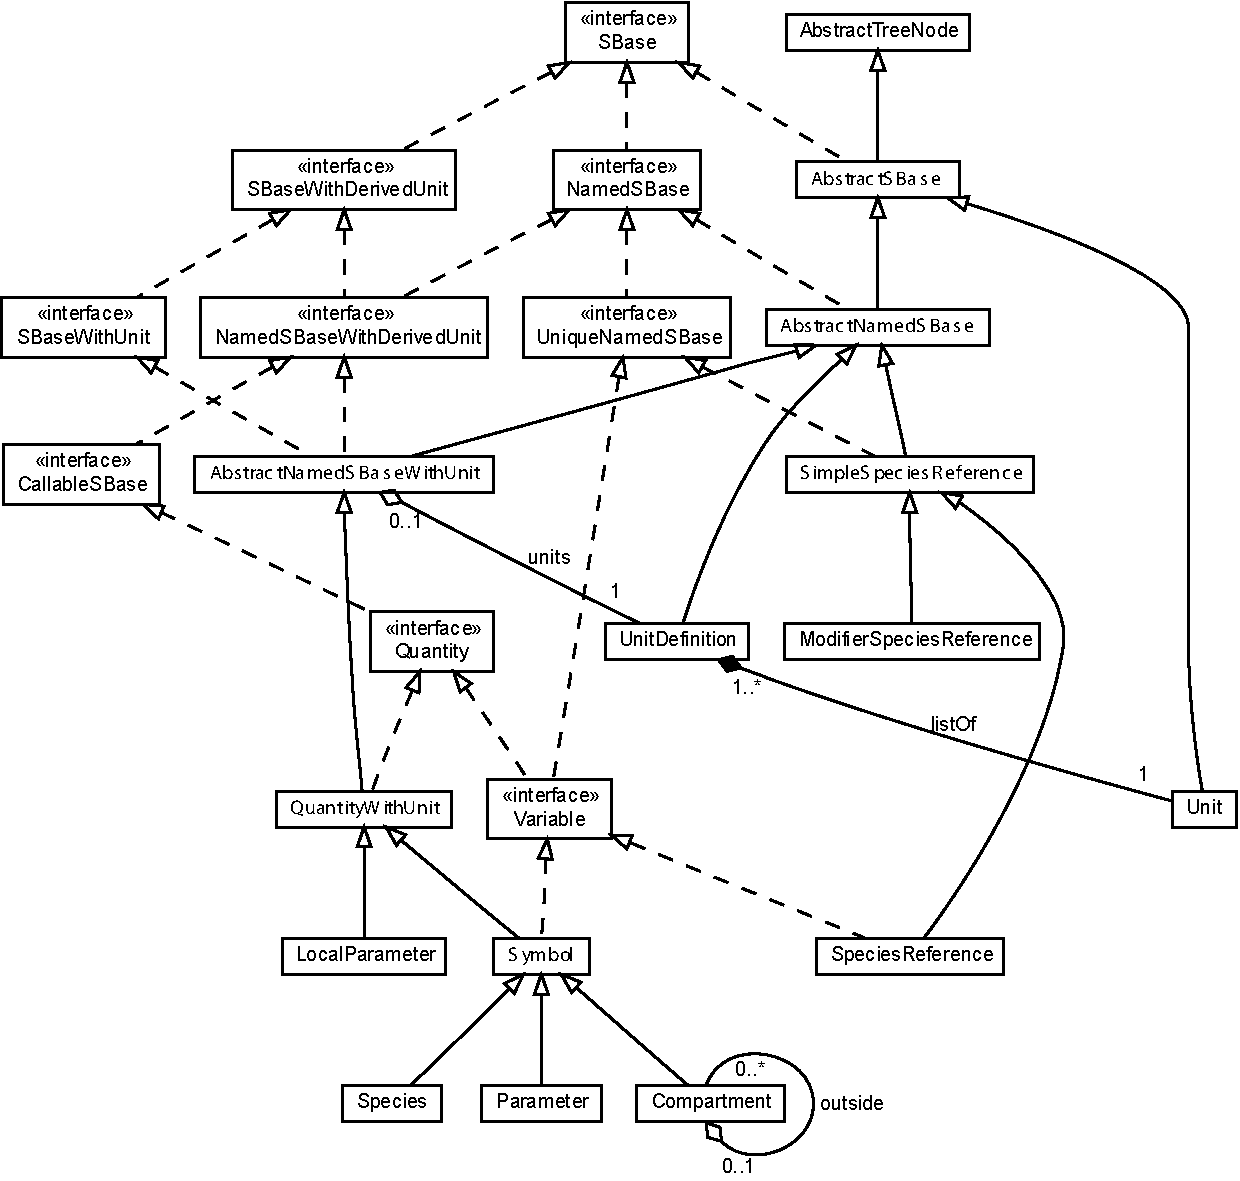
\includegraphics[width=\textwidth]{../common/img/Symbol.pdf}
  % Symbol.pdf: 596x587 pixel, 72dpi, 21.03x20.71 cm, bb=0 0 596 587
  \caption[The interface \Variable]{Part of JSBML's type
    hierarchy focusing on the interface \Variable.  In JSBML,
    those components of a model that may change their value during a
    simulation are referred to as \emph{variables}. The class \Symbol serves
    as the abstract superclass for variables that have units of measurement
    associated with them. Instances of \Parameter do not contain any
    additional fields. In \Species, a Boolean switch decides whether its
    value is to be interpreted as an initial amount or as an initial
    concentration. In contrast to \Variable{}s, \LocalParameter{}s represent
    constant unit-value pairs that can only be accessed within their
    declaring \KineticLaw. \index{SBML!variable}}
 \label{fig:Variable}
\end{figure}


If the SBML component can be addressed with an identifier (which means that
it has an \code{id} field in SBML), it will also implement the JSBML
interface \NamedSBaseWithDerivedUnit, and if it can appear within a formula
(which in JSBML, is represented using \ASTNode, discussed further below),
the entity will further implement the interface \CallableSBase, a special
case of \code{NamedSBaseWithDerivedUnit}.  When a component can be assigned
a unit explicitly, in JSBML the \SBaseWithUnit serves as its superclass.
JSBML further defines the convenience class \AbstractNamedSBaseWithUnit; it
extends \AbstractNamedSBase and implements interfaces \SBaseWithUnit
and \NamedSBaseWithDerivedUnit.  All elements derived from this abstract
class may therefore declare a unit and can be addressed using an
unambiguous SBML identifier.

In JSBML, the interface \Quantity describes an element that is associated
with a value, has at least a derived unit, and can be addressed using its
unambiguous identifier. JSBML uses the abstract class \QuantityWithUnit for
a \Quantity that explicitly declares its unit.  If the corresponding SBML
component includes a Boolean \index{Boolean} flag to indicate whether it is
a constant \index{SBML!constant} or a variable, JSBML
represents such a type using the interface \Variable.

SBML variables \index{SBML!variable} that have a defined unit are
represented as \Symbol objects.  (See \fig{fig:Variable}.) Thus,
the SBML elements \Compartment, \Parameter, and \Species are all special
cases of \Symbol in JSBML.  The specification of \SBMLthree introduced
another type of \Variable, which does not explicitly declare its unit:
\SpeciesReference.  Level~3 also introduced \LocalParameter, which is a
\QuantityWithUnit but not a \Variable because it is always constant.
\sec{sec:assignment-interface} explains the interfaces used for
changing the values of \Variable{}s.


\subsection{Interface for SBML components containing a mathematical
  formula: \codeNC{MathContainer}} 

The interface \MathContainer in JSBML gathers all those elements that may
contain mathematical expressions encoded in abstract syntax trees (i.e.,
instances of \ASTNode).  The abstract class \AbstractMathContainer serves
as actual superclass for the majority of the derived types.
\vrefrange{fig:MathContainer}{fig:MathContainerHierarchy} give a
better overview of how these data structures are organized and how they
relate to each other and other ones in JSBML.

\begin{figure}[hb]
 \centering
 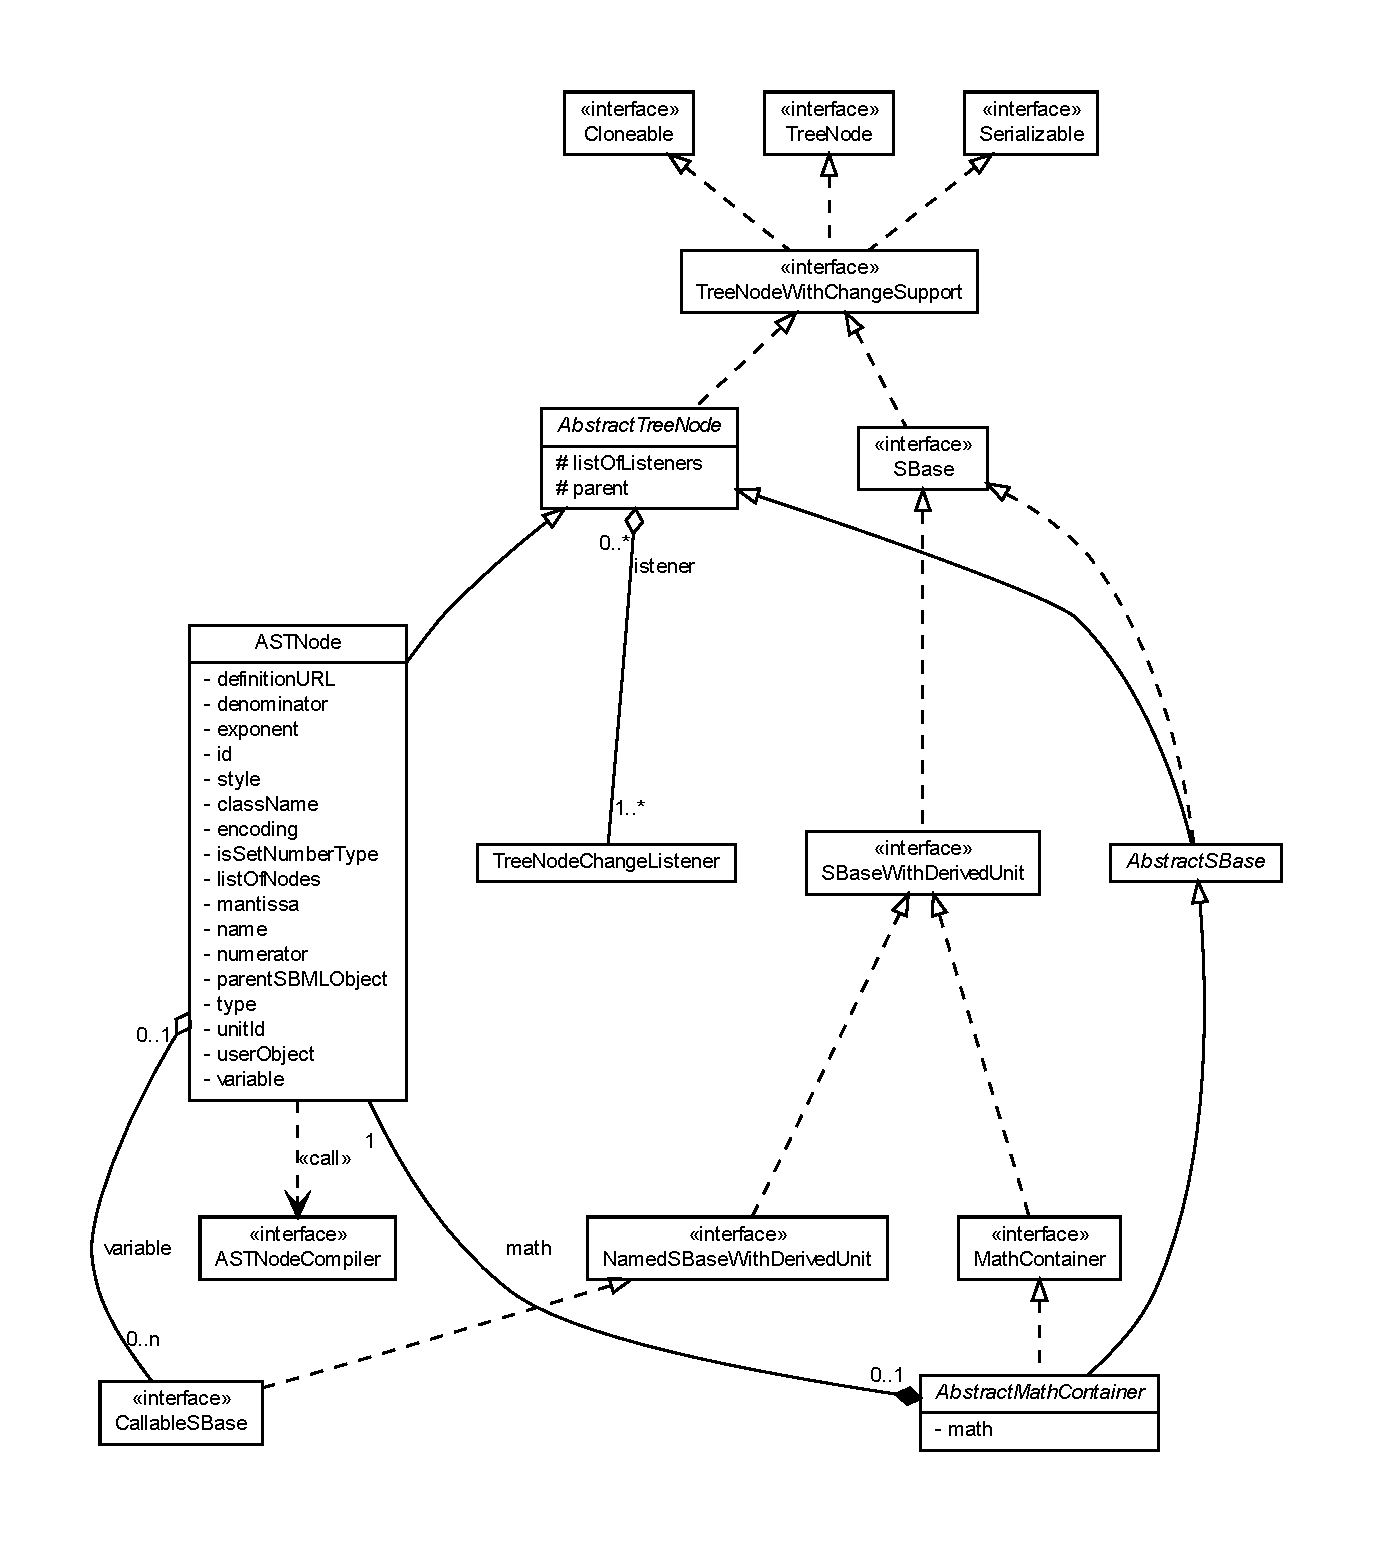
\includegraphics[width=\textwidth]{../common/img/ASTNode.pdf}
 % MathContainerClass.pdf: 557x396 pixel, 72dpi, 19.65x13.97 cm, bb=0 0 557 396
 \caption[Abstract syntax trees]{Abstract syntax trees (ASTs). The class
   \AbstractMathContainer serves as the superclass for several model
   components in JSBML. It provides methods to manipulate and access an
   instance of \ASTNode, which can be converted to or read from text
   strings containing formulas in a C-like infix syntax. Internally,
   \AbstractMathContainer{}s only deal with instances of \ASTNode. It
   should be noted that these abstract syntax trees do not implement the
   \SBase interface, but extend \AbstractTreeNode instead.}
 \label{fig:MathContainer}
\end{figure}

\begin{sidewaysfigure}
 \centering
 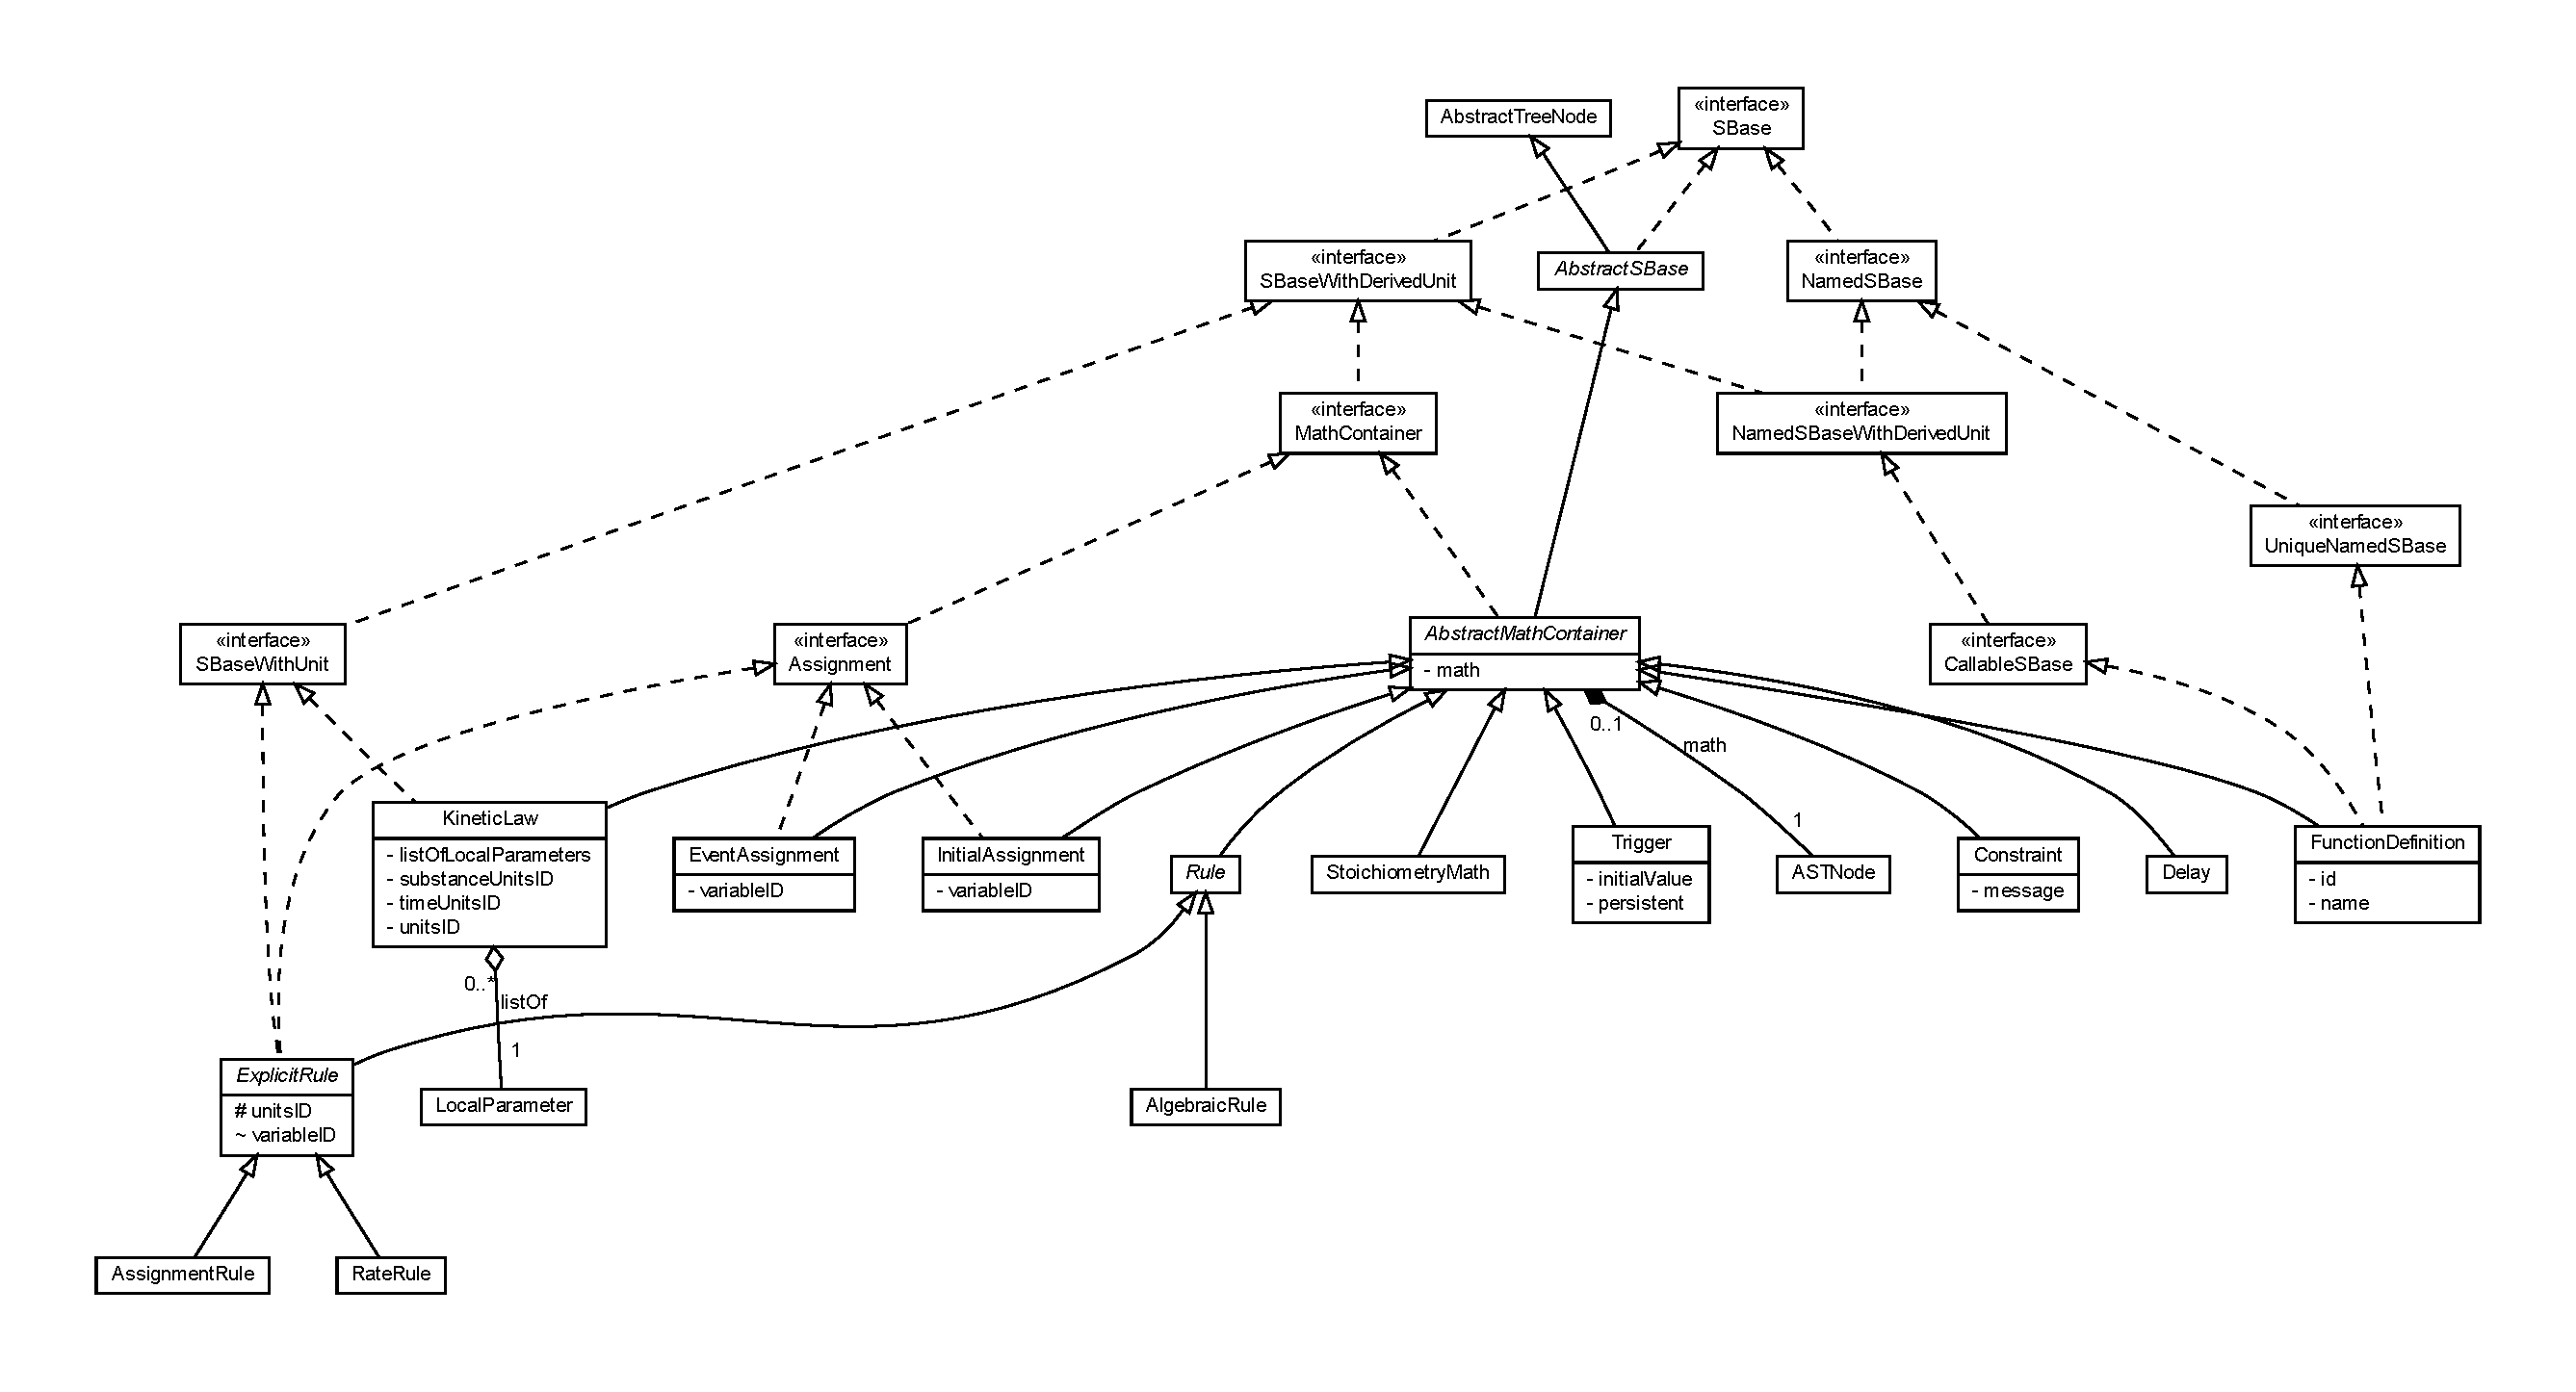
\includegraphics[width=\textwidth]{../common/img/MathContainer.pdf}
 % MathContainerClass.pdf: 557x396 pixel, 72dpi, 19.65x13.97 cm, bb=0 0 557 396
 \caption[Containers for mathematical expressions]{Containers for
   mathematical expressions. The interface \MathContainer, particularly its
   directly derived class \AbstractMathContainer, constitutes the
   superclass for all elements that store and manipulate mathematical
   formulas in JSBML.  The formulas themselves are stored in the form of
   \ASTNode objects. These can be evaluated using an implementation of
   \ASTNodeCompiler. Note that some classes that extend
   \AbstractMathContainer do not contain any of their own additional fields
   or methods.  This is the case for \Delay, \Priority, \StoichiometryMath,
   and \AlgebraicRule.}
 \label{fig:MathContainerHierarchy}
\end{sidewaysfigure}


\subsection{Interface for SBML components that may change the value of
  a variable: \codeNC{Assignment}}
\label{sec:assignment-interface}
\index{JSBML!assignment@\code{Assignment}}

JSBML provides a unified interface, \Assignment, for all objects that may
change the value of some variable in SBML. \index{SBML} This interface uses
the term \emph{variable} for the element whose value can be changed
depending on some mathematical expression that is also present in the
\Assignment (because the interface \Assignment extends the interface
\MathContainer).  Therefore, an \code{Assignment} contains methods such as
\code{set}-/\code{getVariable(Variable v)} and also \code{isSetVariable()}
as well as \code{unsetVariable()}.

In addition, JSBML also provides the methods
\code{set}-/\code{getSymbol(String symbol)} in the \InitialAssignment class
to make it easier to switch from libSBML to JSBML.  However, in JSBML, the
preferred way \index{JSBML!variable@\code{Variable}} is to apply the
methods \code{setVariable()}, either with \String or \Variable instances as
arguments.  \fig{fig:MathContainerHierarchy} shows the class
hierarchy surrounding the \Assignment interface in more detail.

% -*- TeX-master: "User_guide"; fill-column: 75 -*-

\section{Differences between the APIs of JSBML and libSBML}
\label{sec:api-differences}

We strove to make JSBML be closely compatible with libSBML. However,
because of the different programming languages used,
some differences are impossible to overcome.
In other cases, an exact translation from libSBML's C/C++ \index{C}
code to Java would be inelegant and unnatural for Java users,
conflicting with another important goal of JSBML: to provide
an API \index{application programming interface!Java} whose classes and
methods behave, and are organized like, those in other Java libraries.

In this section, we discuss the most important differences in the APIs of
JSBML \index{application programming interface!JSBML} and libSBML.
\index{application programming interface!libSBML} We also provide some
examples of how the classes and methods in JSBML may be used.


\subsection{Level and Version \codeNC{ValuePair}}

In libSBML, the Level and Version information is recorded as individual
integers; by contrast, in JSBML it is stored in a generic object, \ValuePair,
stored within an \AbstractSBase instance. The class \ValuePair implements the
Java interface \Comparable and takes two values of any type that both also
implement \Comparable.  Storing the information in this way allows users to
check for a specific Level/Version combination more naturally, as the example
in \fig{fig:LevelVersionCheck} demonstrates. The method
\code{getLevelAndVersion()} in \AbstractSBase delivers an instance of
\ValuePair with the Level and Version combination for the respective element.

\begin{figure}[bh]%
  \begin{example}
if (mySBase.getLevelAndVersion().compareTo(Integer.valueOf(2), Integer.valueOf(2)) < 0) {
  throw new IllegalArgumentException("Cannot create a " + mySBase.getElementName() + 
  		" with Level = " + getLevel() + " and Version = " + getVersion() + ".");
}\end{example}
  \caption{Example program fragment showing how to check for a minimal
    expected SBML Level/Version combination.}
  \label{fig:LevelVersionCheck}
\end{figure}


\subsection{Abstract syntax trees for mathematical formulas}

Both libSBML and JSBML define a class called \ASTNode for in-memory storage
and evaluation of abstract syntax trees (ASTs) that represent mathematical
formulas. These can be parsed either from \String{}s containing formulas in a
C-like infix syntax, or from a MathML \index{MathML} representation.  JSBML's
\ASTNode class provides various methods to transform ASTs to other formats,
for instance, \code{String}s in \LaTeX \index{LaTeX@\LaTeX} syntax.  Several static methods also
make it easy to create syntax trees.  The next example creates a new
\ASTNode which represents the sum of the two other nodes:

\begin{example}
ASTNode myNode = ASTNode.sum(myLeftAstNode, myRightASTNode);
\end{example}

SBML specifies that mathematical formulas may contain references to the
following kinds of components in a model: \Parameter{}s,
\LocalParameter{}s, \FunctionDefinition{}s, \Reaction{}s, \Compartment{}s,
\Species, and in \SBMLthree, \SpeciesReference{}s.  In JSBML, all of these
classes implement a common interface, \CallableSBase, which extends
the interface \NamedSBaseWithDerivedUnit. This organization ensures that
only identifiers of these particular SBML components can be set in
instances of \ASTNode.


\subsubsection{Constructors and other methods for \CallableSBase}

JSBML provides useful constructors and methods to work with instances of
\CallableSBase.  The \code{set} method changes the type of an \ASTNode to
\ASTTypeName and directly sets the name to the identifier of the given
\CallableSBase.  The \code{get} method looks for the corresponding object in
the \Model and returns it. If no such object can be found or the type of the
\ASTNode is something different from \ASTTypeName, it throws an exception.

\begin{example}[title={Getter and setter for \CallableSBase.}]
public void setVariable(CallableSBase variable) { ... }

public CallableSBase getVariable() { ... }
\end{example}

The following are examples of methods for creating and manipulating complex
ASTs.  JSBML provides several static methods (such as \code{sum} shown above)
that create small trees from objects in memory.  Other methods, such as
\code{plus}, \code{frac} and \code{pow}, change existing tree structures:

\begin{example}[title={Some examples for convenience methods, some of
    them static methods, provided by JSBML for working with \ASTNode{}s.}]
public ASTNode plus(CallableSBase nsb) { ... }

public static ASTNode frac(MathContainer container,
      CallableSBase numerator, CallableSBase denominator) { ... }

public static ASTNode pow(MathContainer container,
      CallableSBase basis, CallableSBase exponent) { ... }
\end{example}

In contrast to the static \code{ASTNode.sum} function at the beginning of
this section, the \code{frac} and the \code{pow} methods above take instances
of \CallableSBase as their arguments instead of \ASTNode objects. Consequently, the
parent \MathContainer must be passed to the methods in order to ensure that
valid data structures are created. (In case of methods that take \ASTNode
objects as arguments, such as the static \code{ASTNode.sum}, the parent
\MathContainer can be taken from the first given node object.)

Finally, with the following \ASTNode constructors, dedicated single nodes can
be created whose type (from the enumeration \ASTType) will be \code{NAME} and
whose name will be set to the identifier of the given \CallableSBase.

\begin{example}
public ASTNode(CallableSBase nsb) { ... }

public ASTNode(CallableSBase nsb, MathContainer parent) { ... }
\end{example}


\subsubsection{The \codeNC{ASTNodeCompiler} class}

JSBML provides the interface \ASTNodeCompiler; it allows users to create
customized interpreters for the contents of mathematical formulas encoded
in abstract syntax trees. It is directly and recursively called from the
\ASTNode class and returns an \ASTNodeValue object, which wraps the
possible evaluation results of the interpretation.  As alluded to above,
JSBML provides several implementations of this interface; for instance,
\ASTNode objects can be directly translated to C language-like \String{}s,
\LaTeX, \index{LaTeX@\LaTeX} or MathML \index{MathML} for further
processing.  In addition, the class \UnitsCompiler, which JSBML uses to
derive the unit of an abstract syntax tree, also implements this interface.


\subsection{Compartments}

In \SBMLthree~\citep{Hucka2010a}, the domain of the attribute
\code{spatialDimensions} on \Compartment is no longer $\lbrace 0, 1, 2,
3\rbrace$, which can be represented with a \code{short} value in Java, and is
instead a real-numbered value (i.e., a value in $\mathbb{R}$), which requires
a \code{double} value in Java. For this reason, the method
\code{getSpatialDimensions()} in JSBML always returns a \code{double}
value. For consistency with libSBML, the \Compartment class in JSBML also
provides the redundant method \code{getSpatialDimensionsAsDouble()} that
returns the identical value; it is marked as a deprecated method.
\index{compartment!\code{getSpatialDimensions()}}%
\index{compartment!\code{getSpatialDimensionsAsDouble()}}%


\subsection{Model history}

Before \SBML Level~3, only the \Model object could have an associated
history, that is, a description about the person(s) who build the model,
including names, email addresses, modification and creation dates.  In
Level~3 of SBML, it is possible to annotate every construct with a
history. This is reflected in JSBML by the name of the corresponding
object---\History---whereas it is named \ModelHistory in libSBML.  All
instances of \SBase in JSBML contain methods to access and manipulate its
\History. Also, JSBML does not have libSBML's classes \ModelCreator
and \ModelCreatorList because JSBML gathers its \Creator objects in a generic
\code{List<Creator>} in the \History.


\subsection{Units and unit definitions}
\label{sec:units}

There are differences between libSBML and JSBML's interfaces for handling
units.  We describe them next.


\subsubsection{The exponent attribute of units}

In \SBMLthree~\citep{Hucka2010a}, the data type of the exponent attribute
of a \Unit object changed from \code{int} in previous Levels to
\code{double} values. To provide a uniform interface no matter which Level
of SBML is being dealt with, JSBML's method \code{getExponent()} only
returns \code{double} values. In libSBML, \code{getExponent()} always
returns \code{int}, and there is an additional method,
\code{getExponentAsDouble()}, to handle the cases with \code{double}
values.  JSBML provides \code{getExponentAsDouble()} for compatibility with
libSBML, but it is a redundant method in JSBML's case and therefore is marked
as deprecated.
\index{unit!getExponent()@\code{getExponent()}}%
\index{unit!getExponentAsDouble()@\code{getExponentAsDouble()}}%


\subsubsection{Predefined unit definitions}

A model in JSBML \index{unit!predefined units} always contains all
predefined units defined by SBML.  These can be accessed from an instance
of \code{Model} by calling the method \code{getPredefinedUnit(String
  unit)}.

MIRIAM annotations\index{annotations!MIRIAM} \citep{Novere2005} have been
an integral part of SBML models since Level~2 Version~2\index{SBML!Level~2
  Version~2}. Recently, the \index{Ontology} Unit Ontology
(UO)~\citep{unitontology} \index{annotations!unit ontology} has been
included in the set of supported ontology and online resources of MIRIAM
annotations~\citep{Novere2005}. Since all the predefined units in SBML have
corresponding entries in the UO, JSBML \index{unit!MIRIAM annotation}%
automatically equips those predefined units with the correct MIRIAM URI in
form of a controlled vocabulary term (\code{CVTerm}) if the SBML
Level/Version combination of the model supports MIRIAM annotations.  In
addition, the \code{enum} \code{Unit.Kind}
\index{unit!Unit.Kind@\code{Unit.Kind}}%
also provides methods to directly obtain the entry from the UO that
corresponds to a certain unit kind and also contains methods to generate
MIRIAM URIs accordingly. In this way, JSBML facilitates the annotation of
user-defined units and unit definitions with MIRIAM-compliant
\index{annotations!MIRIAM} information.


\subsubsection{Access to the units of an element}

In JSBML, all SBML components whose value can be associated with a unit of
measurement implement the interface \SBaseWithUnit.  This interface provides
methods to access an object representing the unit. Currently, the interface
is implemented by \AbstractNamedSBaseWithUnit, \ExplicitRule, and
\KineticLaw.  \fig{fig:TypeHierarchy} provides an overview about the
relationships between these and other classes and interfaces.

% FIXME

\AbstractNamedSBaseWithUnit is the abstract superclass for \Event and
\QuantityWithUnit.  In the class \Event, all methods to deal with units are
deprecated because the \code{timeUnits} attribute was removed in SBML
Level~2 Version~2\index{SBML!Level~2}. The same holds true for instances of
\ExplicitRule and \KineticLaw which both can only be explicitly populated
with units in SBML Level~1\index{SBML!Level~1} for \ExplicitRule and before
SBML in Level~2, Version~3\index{SBML!Level~2} for \KineticLaw. By
contrast, the abstract class \QuantityWithUnit serves as the superclass for
\LocalParameter and \Symbol, which is then the superclass of \Compartment,
\Species, and (global) \Parameter.  With \SBaseWithUnit being a subclass of
\SBaseWithDerivedUnit, users can access the units of such an element in two
different ways:

\begin{description}[font=\normalfont]

\item[\code{getUnit()}:] This method returns a \String representation of
  the unit kind or the identifier of a unit definition in the model \index{model} that has
  been directly set by the user during the life time of the element. If
  nothing has been declared, this method returns an empty \String.

\item[\code{getDerivedUnit()}:] This method gives either the same
  result as \index{unit!derived unit} \code{getUnit()} if some unit has
  been declared explicitly, or it returns the predefined unit of the
  element for the given SBML Level/Version combination.  If neither a
  user-defined nor a predefined unit is available, this method returns an
  \index{String@\code{String}!empty} empty \String.

\end{description}

% FIXME

For convenience, JSBML also provides corresponding methods to the ones
above for directly obtaining an instance of \UnitDefinition.  However, care
must be taken when obtaining an instance of \UnitDefinition from one of the
classes implementing \SBaseWithUnit because it might happen that the
model\index{model} containing this \SBaseWithUnit does actually not contain
the required instance of \UnitDefinition and the method returns a
\code{UnitDefinition} that has just been created for convenience from the
information provided by the class. It might therefore be useful for callers
to either check if the \Model{} contains this \UnitDefinition or to add it
to the \Model.

In case of \KineticLaw it is even more difficult, because SBML
Level~1\index{SBML!Level~1} provides the ability to set the substance unit
and the time unit separately. To unify the API
\index{application programming interface!JSBML}, we decided to also provide methods that
allow the user to simply pass one \UnitDefinition or its identifier to
\KineticLaw.  These methods then try to guess if a substance unit or time
unit is given. Furthermore, it is possible to pass a \UnitDefinition
representing a variant of substance per time directly. In this case, the
\KineticLaw will memorize a direct link to this \UnitDefinition in the
model\index{model} and also try to save separate links to the time unit and
the substance unit. However, this may cause a problem if the containing
\Model does not contain separate \UnitDefinition{}s for both entries.


\subsection{Cloning when adding child nodes to instances of \codeNC{SBase}}

When adding elements such as a \Species to a \Model, libSBML \index{cloning}
will clone the object and add the clone to the \Model. In contrast, JSBML
does not automatically perform cloning. This has the advantage that
modifications on the object belonging to the original pointer will also
propagate to the element added to the \Model; furthermore, this is more
efficient at run-time and also more intuitive for Java programmers. If
cloning is necessary, users should call the \code{clone()} method
explicitly. Since all instances of \SBase, and also \Annotation, \ASTNode,
\CVTerm, and \History, extend \AbstractTreeNode (which in turn implements the
interface \Cloneable---see \fig{fig:TypeHierarchy}), all these elements can
be cloned naturally.  However, when cloning an object in JSBML
\index{cloning}, such as an \AbstractNamedSBase, all children of this element
will recursively be cloned before adding them to the new element. This is
necessary because the data structures specified in SBML
\index{SBML!hierarchical structure} define a tree, in which each element has
exactly one parent. It is important to note that some properties of the
elements must not be copied when cloning:

\begin{enumerate}

\item The pointer to the parent node of the top level element that is
  recursively cloned is not copied and is left as \code{null}, because the
  cloned object will get a parent set as soon as it is added or linked again
  to an existing tree. Note that only the top-level element of the cloned
  subtree will have a \code{null} value as its parent. All subelements will
  point to their correct parent element.

\item The list of \TreeNodeChangeListener objects is used in all other
  \code{setXX()} methods. Copying pointers to these may lead to
  unexpected behaviors, because during deep cloning, the listeners of
  the old object will suddenly be informed about all changes to values within
  the new object.  In cloning, all values of all child elements
  will be touched, i.e., all listeners will have to be informed many times, but
  each time they will receive the same value. Since they do not
  extend the \Cloneable interface, we cannot clone them either; for this reason, the cloned
  object has no \TreeNodeChangeListener object attached to it. The user is responsible
  for adding \TreeNodeChangeListener{}s on the cloned object if they want to be
  notified of any changes to it.

\item Since release 1.0, JSBML supports storing user objects in any object
  derived from \AbstractTreeNode.  These user objects are organized in a map
  data structure with object as key type, pointing to arbitrary user-defined
  objects. Note that generally no deep cloning of these user objects is
  possible, but JSBML keeps a pointer to these user objects in the cloned
  element.

\end{enumerate}


\subsection{Exceptions}
\label{sec:exceptions}

In case of an error, JSBML \index{exception} methods will usually throw an
exception, whereas libSBML \index{exception!error codes} methods return a
numeric error code instead. The libSBML approach is rooted in the need to
support C-like languages, while exception handling is more natural in Java.
The JSBML approach of using exceptions helps programmers and users to avoid
creating invalid SBML data structures already when dealing with these in
memory. 

As per usual Java practice, JSBML methods declare that these may
potentially throw exceptions. In this way, programmers can be aware of
potential sources of problems already at the time of writing the source
code. Examples of the kinds of exceptions that JSBML methods may throw
include \ParseException, \index{exception!\code{ParseException}} which may
be thrown if a given formula cannot be parsed properly into an \ASTNode
data structure, and \InvalidArgumentException,
\index{exception!\code{InvalidArgumentException}} which may be thrown if
inappropriate values are passed to methods.

The following are some examples of situations that lead to exceptions:

\begin{itemize}

\item An object representing a constant\index{constant} such as a
  \Parameter whose \code{constant} attribute has been set to \code{true}
  cannot be used as the \Variable element in an \Assignment.
  \index{JSBML!assignment@\code{Assignment}}%
  \index{JSBML!variable@\code{Variable}}%
  \index{parameter!\code{Parameter}}%
  \index{parameter!\code{constant}}%

\item An instance of \Priority can only be assigned to an \Event{}s if its
  \code{level}\index{SBML!Level~3} attribute has at least been set to
  three.

\item Another example is the \InvalidArgumentException that is thrown when
  trying to set an invalid identifier \String for an instance of
  \AbstractNamedSBase.

\item JSBML keeps track of all identifiers within a model. For each
  namespace it contains a separate map of identifiers within the \Model. It
  is therefore not possible to assign duplicate identifiers in case of
  elements that implement the interface \UniqueNamedSBase.  For
  \UnitDefinition{}s and \LocalParameter{}s separate maps are
  maintained. Since local parameters are only visible within the
  \KineticLaw that contain these, JSBML will only prohibit having more
  than one local parameter within the same list that has the identical
  identifier. All these maps are updated upon any changes within the
  model. When adding an element with an already existing identifier for its
  namespace, or changing some identifier to a value that is already defined
  within this namespace, JSBML will throw an exception.

\item ``Meta'' identifiers must be unique through the entire SBML file. To
  ensure that no duplicate meta identifiers are created, JSBML keeps a map
  of all meta identifiers on the level of the \SBMLDocument, which is
  updated upon any change of elements within the data structure. In this
  way, it is not possible to map the meta identifier of some element to an
  already existing value or to add nodes to the SBML tree that contain a
  meta identifier defined somewhere else within the tree. In both cases,
  JSBML will throw an exception. Since meta identifiers can be generated in
  a fully automatic way (method \code{nextMetaId()} on
  \code{SBMLDocument}), users of JSBML should not care about these
  identifiers at all. JSBML will automatically create meta identifiers
  where missing upon writing an SBML file.  (See \sec{sec:find-methods}.)

\item In case that spatial dimension units of a \Species{} are defined
  whose surrounding \Compartment{} has zero dimensions or that has only
  substance units, JSBML also throws an exception.

\end{itemize}

Hence, you have to be aware of potential exceptions and errors when using
JSBML, \index{exception} on the other hand this will prevent you from doing
obvious mistakes. The class \SBMLReader in JSBML catches those errors and
exceptions. With the help of the logging utility, JSBML notifies users
about syntactical problems in SBML files. JSBML follows the rule that
illegal or invalid properties are not set.


\subsection{No interface  \codeNC{libSBMLConstants}}

JSBML does not contain an equivalent to libSBML's
\code{libSBMLConstants}. The reason is that in JSBML, constants are encoded
in a more natural Java fashion, \index{constant!\code{enum}}%
using the Java construct \code{enum}. For instance, all the fields starting
with the prefix \ASTTypePrefix{} have a corresponding field in the \ASTNode
class itself.   There you can find the enumeration \ASTType.  Thus, instead of typing
\code{libSBMLConstants.AST\_TYPE\_PLUS}, you type
\code{ASTNode.Type.PLUS}.  The same holds true for \code{Unit.Kind.*}
corresponding to the \code{libSBMLConstants.UNIT\_KIND\_*}
\index{unit!UNIT\_KIND\_*@\code{UNIT\_KIND\_*}}%
fields.

\subsection{No class \codeNC{libSBML}}

JSBML contains no class called \code{libSBML} simply because the library
is called \emph{JSBML}.  \index{libSBML!libSBML@\code{libSBML}}%
In its place, there is a class named \code{JSBML}.
\index{JSBML!JSBML@\code{JSBML}} This class provides some methods similar
to the ones provided in libSBML's \code{libSBML}, such as
\code{getJSBMLDottedVersion()} \index{JSBML!version}%
to obtain the current version of the JSBML library, which is 0.8 or 1.0-a* at the
time of writing this document. However, many other methods that you might
expect to find there, if you are used to libSBML, are located in the actual
classes that are related with the function. 

Here is an example of a method that is located on the relevant class.  To
convert between a \String \index{unit!String@\code{String}}%
and a corresponding \code{Unit.Kind}
\index{unit!Unit.Kind@\code{Unit.Kind}}%
you would use the following:

\begin{example}[title={Converting a string to a unit kind in JSBML.}]
Unit.Kind myKind = Unit.Kind.valueOf(myString);
\end{example}

Analogous to the above, the \ASTNode class provides a method to parse
C-like infix formula {\String}s according to the specification of SBML
Level~1~\citep{Hucka2003}\index{SBML!Level~1} into an abstract syntax
tree. Therefore, in contrast to the \code{libSBML} class, the class
\code{JSBML}\index{JSBML!JSBML@\code{JSBML}} contains only a few methods.


\subsection{No individual \codeNC{ListOf*} classes, but a generic \codeNC{ListOf}}

% We have the method get(String) on the ListOf and libsbml does not have it on
% the main ListOf class, only on subclasses where it is possible to do it.

JSBML does not have a specific \code{ListOf*}\index{ListOf*@\code{ListOf*}}
class for each type of \SBase elements, which is unlike the case in
libSBML. In JSBML, we use a generic implementation \code{ListOf<?~extends
  SBase>} that enables the same class to be used for each of the different
\code{ListOf*} classes defined in SBML while keeping a type-safe class.

To help developers work with \code{ListOf*} lists more conveniently, JSBML
provides several methods that use the Java \code{Filter} interface to search
and filter the lists. For example, to query an instance of a \code{ListOf*}
list in JSBML for specific identifiers, or names, or both, you can apply the
following filter:

\begin{example}[title={Example of searching a list for an object with a
    particular identifier.}]
NamedSBase nsb = myList.firstHit(new NameFilter(identifier));
\end{example}

This will return the first element in the list with the given identifier.  In
SBML, a \code{ListOf*} list object usually must not contain multiple elements
with the same identifier, so the element will usually be unique.  The
\code{firstHit} method stops after finding one element that satisfies the
given \code{Filter}. The \code{ListOf<?~extends SBase>} class also offers a
\code{filter} method that takes a \code{Filter} object as argument and
collects all elements accepted by that \code{Filter} object.

Various filters are already implemented in JSBML and made available for use
in your programs, but you can easily add your own custom filter. You only
need to implement the \Filter interface defined in the JSBML package
\code{org.sbml.jsbml.util.filters}.  In that package, you can also find an
\OrFilter and an \AndFilter, which take as arguments multiple other
filters. With the \SBOFilter you can query for certain SBO annotations
\citep{Novere2006, Novere2006b} \index{annotations!SBO}%
in your list; similarly, the \CVTermFilter helps you to identify \SBase
instances with a desired MIRIAM (Minimal Information Required In the
Annotation of Models) annotation~\citep{Novere2005}\index{annotations}. For
instances of \code{ListOf<Species>}, you can apply the
\BoundaryConditionFilter to look for those species\index{species!boundary
  condition} that operate on the boundary of the reaction system.


\subsection{Use of deprecation}

The intention of JSBML\index{JSBML!deprecation} is to provide a Java
library that supports the latest specifications of SBML\index{SBML}.
\index{SBML!specification}%
\index{deprecation}%
But we also want to support earlier specifications. So JSBML provides
methods and classes to cover elements and properties from earlier SBML
specifications as well, but these are often marked as being deprecated to
help users avoid creating models that refer to these elements. 

JSBML also contains many methods added for greater compatibility with
libSBML, but which programmers would probably not use unless they were
transitioning existing software from libSBML.  For instance, a method such
as \code{getNumXyz()} is not considered to be very Java-like (but such
methods are common for a C++\index{C++} programming style). Usually, Java
programmers would expect the method being called \code{getXyzCount()}
instead. For cases like this, JSBML provides alternative methods and marks
these methods that originate from libSBML as deprecated.



\chapter{Additional features provided by JSBML}
\label{chp:additional-jsbml-features}

The previous chapter covered many features of the JSBML API and how they
compare to those provided by libSBML's API.  In addition to the features
described in that chapter, JSBML also provides a number of capabilities that
are not found in libSBML.  This chapter briefly introduces the most important
additional capabilities.

% -*- TeX-master: "User_guide"; fill-column: 75 -*-

\section{Change listeners}

JSBML offers the ability to listen to change events in the life of an SBML
document. To benefit from this facility, simply let your class implement
the interface \TreeNodeChangeListener and add it to the list of listeners
in your instance of \SBMLDocument. You only have to implement three
methods:

\begin{description}[font=\normalfont]

\item[\code{nodeAdded(TreeNode node)}:] This method notifies the listener
  that the given \TreeNode instance has just been added to the \SBMLDocument
  object. When this method is called, the given node is already fully linked
  to the \SBMLDocument, i.e., it has a valid parent that in turn points to
  the given node.

\item[\code{nodeRemoved(TreeNodeRemoveEvent evt)}:] This method notifies the listener
  that a \TreeNode has just been removed, and therefore is
  no longer part of the \SBMLDocument. The deleted element can be accessed 
  using the \code{getSource()} method of the given event object. The 
  \SBMLDocument will no longer contain
  pointers to this node; however, the event object will contain
  a pointer to its former parent, and it can be accessed by calling \code{getPreviousParent}
  on the event object. (This makes it possible to recognize where
  in the tree this node was located and even to revert the deletion of the
  node.)

\item[\code{propertyChange(PropertyChangeEvent evt)}:] This method
  provides detailed information about the change in a value within the
  \SBMLDocument.  The object passed to this method is a
  \TreeNodeChangeEvent, which provides information about which \TreeNode
  has been changed, which of its properties has been changed (as a
  \String representation of the name of the property), the previous value,
  and the new value.

\end{description}

These methods can help software track what their \SBMLDocument objects are
doing at any given time.  Furthermore, these features can be very useful in
a graphical user interface\index{graphical user interface}, where, for
example, the user might need to be asked if he or she really wants to
delete some element or to approve changes before making these
persistent. Another way this can be used is for writing log
files\index{logging!log file} of the model-building \index{model} process
automatically. To this end, JSBML already provides the implementation
\SimpleTreeNodeChangeListener which notifies a logger about each change.

Note that the class \TreeNodeChangeEvent extends the class
\code{java.beans.Property\-Change\-Event},
\index{event!PropertyChangeEvent@\code{PropertyChangeEvent}} which is
derived from
\code{java.util.EventObject}\index{event!EventObject@\code{EventObject}}.
It should also be pointed out that the interface \TreeNodeChangeListener
extends the interface \code{java.beans.Pro\-perty\-Change\-Listener}
\index{event!PropertyChangeListener@\code{PropertyChangeListener}} which in
turn extends the interface \EventListener in the package
\code{java.util}. In this way, the event and listener data structures fit
into common Java API idioms \index{application programming interface!Java}
and allow users also to make use of, e.g., \EventHandler{}s to deal with
changes in an SBML model\index{model}.

As mentioned in \sec{sec:AbstractTreeNode}, all major objects implement
the interface \TreeNode, and its listeners are notified about all changes
that occur in any implementing data structure. The use of
\TreeNodeChangeListener{}s allows a software application not only to keep
track of changes in instances of \SBase, but also changes inside of, e.g.,
\CVTerm or \History.

% -*- TeX-master: "User_guide"; fill-column: 75 -*-

\section{Determination of the variable in \codeNC{AlgebraicRule}s}

JSBML's \OverdeterminationValidator provides methods to determine if a given
model\index{model!over determination} is overdetermined; it uses the
algorithm of Hopcroft and Karp~\cite{Hopcroft1973}.

\OverdeterminationValidator simultaneously determines the free variable of
each \AlgebraicRule if possible. The class \AlgebraicRule also provides a
convenience method, \code{getDerivedVariable()}, to compute and return this
free variable.  However, we do not recommend calling this method except in
limited circumstances, because each call invokes the matching algorithm---an
operation that may be expensive for large models. JSBML does not store the
results of applying the matching algorithm because a change in the model's
structure could also change these results and lead to an inconsistency.  For
models that contain multiple \AlgebraicRule objects, it is instead more
efficient to compute the matching once by invoking
\OverdeterminationValidator. Please see the documentation for \AlgebraicRule
for more details.


% -*- TeX-master: "User_guide"; fill-column: 75 -*-

\section{The \codeNC{find*} methods}
\label{sec:find-methods}

JSBML provides developers with a number of \code{find*} methods
\index{JSBML!\code{find*} methods}%
on a \Model to help query for elements based on their identifiers or
names. Software can search for various instances of \code{SBase} (for
instance, \CallableSBase, \NamedSBase, and \NamedSBaseWithDerivedUnit);
using methods such as \code{findLocalParameters}, \code{findQuantity},
\code{findQuantityWithUnit}, \code{findSymbol}, and \code{findVariable},
software can also search for the corresponding model element.  They enable
software to work with SBML models more easily, without the need for
explicit separate iteration loops for these common operations.

As of JSBML version 1.0, the \code{find*} methods do no longer query the
model in an iterative way. Instead, the maps described in
\sec{sec:exceptions} are used to access elements based on their \code{id}
attribute. Similarly, the \SBMLDocument can also directly access any of its
subelements for a given \code{metaid}. Such a search can be performed in
logarithmic runtime, i.e., $O(\,\log_2 n)$.


% -*- TeX-master: "User_guide"; fill-column: 75 -*-

\section{Other utility classes provided by JSBML}

JSBML also provides additional utility classes besides those mentioned
above. In the paragraphs below, we describe some of these classes in more
detail.  All of them are gathered in the package
\code{org.sbml.jsbml.util}, where you can also find a growing number of
additional helpful classes.

\subsection{Mathematical functions and constants}

The class \code{org.sbml.jsbml.util.Maths}
\index{JSBML!Maths@\code{Maths}}%
contains several static methods for mathematical operations not provided by
the standard Java class \code{java.lang.Math}. Most of these methods are
basic operations, for instance, \code{cot(double x)} or \code{ln(double
  x)}.  The JSBML class \code{Maths} also provides some less commonly used
methods, such as \code{csc(double x)} or \code{sech(double x)} as well as
\code{double} constants representing Avogadro's number and the universal
gas constant
$R = 8.314472\;\mathrm{J}\cdot\mathrm{mol}^{-1}\cdot\mathrm{K}^{-1}$.
In this way, the functions and constants implemented in class \code{Maths}
complement standard Java with methods and numbers required by the SBML
specifications~\citep{Hucka2003, Hucka2008, Hucka2010a}.

\subsection{Some tools for \codeNC{String} manipulation}

The JSBML class \StringTools provides several methods for convenient
\String manipulation. These methods are particularly useful when parsing or
displaying \code{double} numbers in a \code{Locale}\hyp{}dependent way. To
this end, this class predefines a selection of useful number formats. It
can also wrap \String elements into HTML code, mask non-ASCII characters
using corresponding HTML codes, efficiently concatenate \String{}s, or
deliver the operating system-dependent new line character.


% -*- TeX-master: "User_guide"; fill-column: 75 -*-

\section{Logging facilities}
\index{logging}%

JSBML includes the logger provided by the log4j
project~\citep{log4j}.  Log4j allows us to use six levels of logging
(\code{TRACE}, \code{DEBUG}, \code{INFO}, \code{WARN}, \code{ERROR}, and
\code{FATAL}) but internally, JSBML mainly uses \code{ERROR}, \code{WARN},
and \code{DEBUG}. The default configuration of log4j used in JSBML can be
found in the folder \code{resources} with the name \code{log4j.properties}.
In this file, you will find some documentation of which JSBML classes do
some logging and at which levels.
 
If a software package using JSBML does not change the default settings, all
the log messages, starting at the info level (meaning info, warn, error and
fatal), will be printed on the console.  Some of these messages might be
useful to warn end-users that something has gone wrong.


\subsection{Changing the log4j configuration}

If you want to modify the default log4j behavior, you will need to create a
custom log4j configuration file. The best way to do this, as described in
the log4j manual~\citep{log4j}, is to use the environment variable
\code{log4j.configuration} to point to the desired configuration file. One
way to accomplish this is to add the following option to your \code{java}
command (shown here for Unix/Linux and Mac~OS~X, but other operating
systems have analogous facilities):

\begin{example}[style=bash, title={Command line option making log4j
    use a different configuration file.  This syntax applies to Unix-like
    systems.}] 
-Dlog4j.configuration=/home/user/myLog4j.properties
\end{example}


\subsection{Some example configurations}
\ifthenelse{\boolean{includeCodeExample}}{}{\index{logging!configuration}}%

\fig{fig:log4j-simple-example} gives a short example of a log4j
configuration file.  The effect of this particular configuration is to
change the threshold of all loggers in the \code{org.sbml.jsbml.util}
package to \code{DEBUG}, which results in all changes that happen to SBML
elements to be logged. The class \SimpleTreeNodeChangeListener{}  will then
output the old value and the new value whenever a setter methods is used on
the SBML elements.

\begin{figure}[t]
  \exampleFile[style=bash, numbers=left, caption={}]{src/log4j_debug_example.properties}
  \caption{A simple log4j configuration example.  This sets the logging
    level of loggers in the \code{org.sbml.jsbml.util} to \code{DEBUG},
    causing all changes to SBML elements to be logged.}
  \label{fig:log4j-simple-example}
\end{figure}

If your application is deployed in a server such as Tomcat~\cite{tomcat},
it may be useful to define a log4j ``appender'' that will send some
messages by email.  \fig{fig:log4j-email-example} gives an example
of doing this.  It configures log4j so that any messages at the
\code{ERROR} level \index{logging} are send by mail. All the messages are
also written to a rolling log file.

Note that using log4j's alternative, XML-based approach to defining
configurations instead of a properties file, you can configure log4j to
direct some log messages \index{logging}%
to one appender and others to an other appender, using the
\code{LevelRange} filter. In this way, it would be possible to cause
\code{DEBUG} messages to be written to a separate file.

\begin{figure}[t]
  \exampleFile[style=bash, numbers=left, caption={}]{src/log4j_email_example.properties}
  \caption{Example of configuring log4j to send email messages for log
    events at the \code{ERROR} level.}
  \label{fig:log4j-email-example}
\end{figure}

Finally, be warned that when you enable the debug level \index{logging} on
some loggers, they may produce copious output.  You may wish to investigate
some of the freely-available software for log
viewing~\cite{logViewersWebpage} to work with the log files.


% -*- TeX-master: "User_guide"; fill-column: 75 -*-

\section{JSBML modules}
\label{sec:jsbml-modules-details}

JSBML modules extend the functionality of JSBML and are provided as
separate libraries (packaged as JAR files). With the help of the current
JSBML modules, JSBML can be used, for example, as a communication layer
\index{JSBML!as communication layer} between your application and
libSBML~\citep{Bornstein2008} or between your program and the program known
as CellDesigner~\citep{Funahashi2003}. In addition, JSBML is planning to offers a
compatibility module \index{libSBML!compatibility module}%
that helps to write code compatible with libSBML by providing the same package 
structure and API as libSBML's Java
language interface. In the rest of this section, we provide examples of how
to use these modules.


\subsection{The \codeNC{libSBMLio} module: using libSBML for parsing
  SBML into JSBML data structures}

The capabilities of the SBML validator\index{SBML!validator} constitutes one
of the major strengths of libSBML~\citep{Bornstein2008} in comparison to
JSBML, which does not yet contain a standalone validator for SBML, but makes
use of the online validation provided at \url{http://sbml.org}. However, if
the platform-dependency of libSBML does not hamper your application, or you
want to switch slowly from libSBML to JSBML, you may still read and write
SBML models using libSBML in conjunction with JSBML.

To facilitate this, the module \code{libSBMLio} provides the classes
\LibSBMLReader and \LibSBMLWriter.  \fig{lst:LibSBMLio} provides a short
code example illustrating the use of \LibSBMLReader.  The program displays the
content of an SBML file in a \JTree, similar to what is shown in
\fig{fig:JSBMLvisualizer-output}.

As of version 1.0 of JSBML, the \code{libSBMLio} module also contains
specialized \TreeNodeChangeListener{}s that synchronize any change in the
JSBML data structure with corresponding libSBML data structures.

\begin{figure}[htb]
  \lstinputlisting[language=Java, style=Java, firstline=33]{src/org/sbml/jsbml/xml/libsbml/libSBMLio_example.java}
  \caption{A simple example showing how to convert libSBML data structures
    into JSBML data objects.  To run this example, you need libSBML
    installed on your system.  You may need to set environment variables,
    e.g., the \code{LD\_LIBRARY\_PATH}
    \index{libSBML!LD\_LIBRARY\_PATH@\code{LD\_LIBRARY\_PATH}}%
    under Linux\index{operating system}, to values appropriate for your
    system. For details, please see the libSBML
    documentation~\cite{libSBMLwebsite}.}
  \label{lst:LibSBMLio}
\end{figure}


\subsection{\textls[-20]{The \codeNC{CellDesigner} module: turning a
    JSBML-based application into a CellDesigner plugin}}

Once an application has been implemented based on JSBML, it can easily be
accessed from CellDesigner's plugin menu~\citep{Funahashi2003}. To support
this, it is necessary to extend two classes that are defined in
CellDesigner's plugin API. 
\index{application programming interface!CellDesigner}
\vrefrange{lst:PluginAction}{lst:Plugin1}
show a simple example of (1) how to pass a model\index{model!CellDesigner}
data structure in a CellDesigner plugin to the translator in JSBML, and (2)
\index{CellDesigner!plugin} \index{CellDesigner!\code{PluginAction}}%
creating a plugin for CellDesigner which displays the SBML data structure
in a tree, like the example in \fig{fig:JSBMLvisualizer-output}.

\exampleFile[firstline=29, caption={A simple implementation of CellDesigner's abstract class \code{PluginAction}.}, label={lst:PluginAction}]{src/org/sbml/jsbml/celldesigner/cdplugin_example.java}

Listings \vrefrange{lst:PluginAction}{lst:Plugin1} show how to translate a
plugin's data structure from CellDesigner into a JSBML data structure. With
the help of the class \PluginSBMLWriter, it is possible to notify
CellDesigner about changes in the data structure. Note that the program in
listing \fig{lst:Plugin1} is only completed by implementing the methods from the
superclass, \code{CellDesignerPlugin}; it is sufficient to leave the
implementation empty.

As of JSBML version 1.0, this module also contains a specialized
implementation of the \TreeNodeChangeListener{} interface for
synchronization of changes in JSBML's data structures with CellDesigner.

\exampleFile[language=Java, style = java, firstline=35, label=lst:Plugin1, caption={A simple example for a CellDesigner plugin using JSBML as a communication layer. Continued in next figure.}]{src/org/sbml/jsbml/celldesigner/SimpleCellDesignerPlugin.java}

\clearpage

\subsection{The \codeNC{libSBMLcompat} module: a JSBML compatibility
  module for libSBML}

The goal of the libSBML compatibility module in JSBML is to provide the
same package structure as libSBML's Java bindings, and provide
identically-named classes and APIs. Using the module, it will be possible
to switch an existing application from libSBML to JSBML or the other way
around without changing any code.  \index{libSBML!compatibility module}%
This module is in early development phase.

\subsection{The \codeNC{android} module: a compatibility module for
  Android systems}
\index{Android}

The JSBML \emph{Android} module is intended to provide all those classes
from the Java standard distribution that are required for JSBML, but might
be missing on Android systems.

\subsection{The \codeNC{compare} module: facilities for doing comparisons between libSBML and JSBML}

During the early development of JSBML, we developed those set of classes in order to check that what
JSBML was reading in memory was equivalent of what libSBML was reading in memory. Those classes were
used (and can still be used) to detect inconsistency between JSBML and libSBML and helped to find bugs
 in both libraries.

\subsection{The \codeNC{tidy} module: to produce a tidy XML output}

The tidy module was created to allow users to write a pretty XML output. In order to use it, you just need to replace
in your code the use of the \SBMLWriter{} class by the \TidySBMLWriter{} class.

% -*- TeX-master: "User_guide"; fill-column: 75 -*-

\section[Offline validation]{The JSBML offline validator}

The JSBML \emph{offline validator} is a self-contained SBML validation facility that implements some of the validation processes included in libSBML.  At the time of this writing, \textbf{the offline validator is incomplete and unsuitable for production use}.  We included it here so that users can experiment with it.  We hope to improve this facility so that in time it can be used to validate SBML files reliably.


\subsection{Basic procedure for using offline validation in JSBML}

The following sections describe the basic steps required to use the offline
validator in your code.


\subsubsection{Create an instance of \codeNC{ValidationContext}}

\code{ValidationContext} is the center of the validation process.  The
constructor for this class requires two arguments, for the Level and Version
of SBML you want to validate. These values can be changed after creating the
context object, but note that doing so will clear any loaded constraints
(discussed below).

\vspace*{1ex}
\begin{example}[style=java, title={Setup a ValidationContext.}]
// Create a new instance
ValidationContext ctx = new ValidationContext(3, 1);
\end{example}

The \code{ValidationContext} is designed to be reusable, so you can use a
single instance of ValidationContext to perform several validations.  To do
so, repeat the next two steps.


\subsubsection{Prepare the context}

Next, provide \code{ValidationContext} with the JSBML SBML objects that you
want to validate. For each such object, use the method
\code{loadConstraintsForClass(Class<?> clazz)} with the objects class as
parameter (e.g., ``\code{object.getClass()}") or by using a static reference
(e.g., ``\code{Species.class}"). The context will traverse the class
hierarchy to load all the constraints that are necessary to achieve
validation. For example, if you use a custom class which is derived from
\Species, the validator will recognize this and also load the constraints for
the \Species class.

\vspace*{1ex}
\begin{example}[style=java, title={Three different ways to load constraints.}]
// Load constraints to validate a MyClass object
ctx.loadConstraintsForClass(MyClass.class);	

// Load constraints to validate the class from myObject
ctx.loadConstraintsForClass(myObject.getClass());

// Load constraints to validate a single attribute
ctx.loadConstraintsForAttribute(myObject.getClass(), "name");

// NOTICE: the loadConstraints methods clears the root constraint.
// After the third command, the context will only contain the constraints to check the "name" attribute.
\end{example}


\subsubsection{Run the validation}

Finally, start the validation procedure. The method \code{validate(Object o)}
will return a Boolean whose value will be \code{true} when no constraint was
broken and \code{false} otherwise.

\begin{example}[style=java, title={Validate.}]
// Perform the validation
boolean isValid = ctx.validate(myObject);
\end{example}

If you invoke the \code{validate} method on an object that is not assignable
to the class for which the constraints were loaded, this method will simply
return \code{false} and print a log message.  To get a list of all the errors
and broken constraints, use an instance of \code{LoggingValidationContext}
instead.


\subsubsection{Control the validation}

There are several ways to control the behavior of the validation process.

\begin{enumerate}

\item \emph{Enable/disable check categories}.  With check categories,
  it's possible to control which subset of rules will be loaded. 

\item \emph{Recursive validation}.  The validation context can perform a
  recursive validation and also validate the child objects. This is realized
  by using the \TreeNode Interface. If a class inherits from \TreeNode (which
  is the case by \SBase) and this option is enabled, the context will also
  load the constraints for the class of every child returned by the \TreeNode
  iteration methods. If one of the children is also a \TreeNode, the
  recursive validation will go on. This option is enabled by default.

\item \emph{Track the validation.}  To follow the validation process in real
  time, use the \code{ValidationListener} interface.  It provides two
  methods:

  \begin{itemize}

  \item \code{willValidate(ValidationContext ctx, AnyConstraint<?> c, Object o)} \\ 
    which is called every time before a constraint will perform a check

  \item \code{didValidate(ValidationContext ctx, AnyConstraint<?> c, Object o, boolean success)} \\
    which is called after the check. The \code{boolean success} will be the result of the check from this constraint.

  \end{itemize}

  If you want to get more information about the constraint, you can retrieve
  its error code. If the constraint is just a \code{ConstraintGroup} and
  therefore just a collection of constraints, the error code should be equals
  to \code{CoreSpecialErrorCodes.ID-GROUP}. In any other case, you could use
  this error code to create the \code{SBMLError} object associated with it
  by using the \code{SBMLErrorFactory}.

\end{enumerate}


\subsection{Providing custom constraints to the offline validator}

It is easy to provide custom constraints. When the \code{ConstraintsFactory}
looks for the constraints for a given class, it uses Java reflection to
search for a constraint declaration for that class. A constraint declaration
is just a simple class that has the name of the class it wants to declare
constraints for, followed by the word ``Constraints''.  For example, the
class that provides the constraints for \Species is called
\code{SpeciesConstraints}. This class must at least implement the
\code{ConstraintDeclaration} interface, but it is best if it also extends
\code{AbstractConstraintDeclaration} because the latter implements most
functions and also caches the constraints.  Notice that any constraint
declaration must be located in the package
``\code{org.sbml.jsbml.validator.offline.constraints}''.

To declare new constraints, follow these steps:

\begin{enumerate}

\item \emph{Create constraint declaration}. First, you have to create the
  class in which you put the code for the constraints and select which
  constraints should be loaded to validate a certain check category.

\begin{example}[style=java, title={Create constraint declaration class}]
// Be sure to use this package, otherwise the ConstraintFactory won't find your constraints.
package org.sbml.jsbml.validator.offline.constraints;

// This class will contain the constraints for a MyClass object
public class MyClassConstraints extends AbstractConstraintDeclaration {
	
	// To be filled with your code...
}
\end{example}

\item \emph{Select the error codes which should be checked}.  Next, you
  have to collect the error codes to perform a proper validation. There are
  two methods, one for the complete validation in a single check category and
  one for the attribute validation. Inside this method, you will have a
  \code{Set<Integer>} to which you should add every error code that should be
  validated in this check category. You could use the level and version
  parameter to avoid loading unnecessary constraints.

\begin{example}[style=java, title={Select error codes}]
  /*
   * In this method you add all the error codes to the set, which should be 
   * covered for the given combination of check category, level and version.
   */
  public void addErrorCodesForCheck(Set<Integer> set, int level, int version,
    CHECK_CATEGORY category) {
    
    switch (category) {
    case GENERAL_CONSISTENCY:
    	// A helper function to add a range to the set (including the last one)
    	addRangeToSet(set, 6, 9);
    		
    	if (level > 1)
    	{
    		set.add(15);
    	}
    
    // other cases...
  	
    }
  }

  /*
   * This method works just like the one above, expect that this time you should
   * collect the error codes to validate only a single attribute of a object.
   *
   * Because the attribute validation is used to catch invalid values in the setters,
   * you should only select error codes which has severity "ERROR" in the given
   *  level and version.
   */
  public void addErrorCodesForAttribute(Set<Integer> set, int level,
    int version, String attributeName) {
	switch (category) {
    case "name":
    	set.add(8);
    	break;
    	
    // other cases...
    
    }
  }
\end{example}

\item \emph{Provide the logic for the constraints}.  Now you only have to
  write the constraint, this is done by providing a validation function. In
  most cases, you will just create an anonymous class and put your code in
  the \code{check(*)} method. This method should return \code{false} if the
  constraint is broken. Keep in mind that the constraints are cached and will
  be reused and shared between different \code{ValidationContext} objects.

  You could avoid caching by using negative numbers as your error codes.
  Beside of this, it's possible (and sometimes necessary) to have different
  constraints with the same error code. Choose your error codes wisely,
  because classes like the \code{LoggingValidationContext} will use the error
  code to load an \code{SBMLError} object for this constraint.

\begin{example}[style=java, title={Select error codes}]
  /*
   * Here you provide the real logic for a constraint in form of a ValidationFunction
   * these function should return true if everything is fine and false otherwise.
   */
  public ValidationFunction<?> getValidationFunction(int errorCode) {
  	ValidationFunction<MyClass> func = null;
  	
  	switch (errorCode){
  	case 4:
  		func  = new ValidationFunction<MyClass> {
  		
  			public boolean check(ValidationContext ctx, MyClass mc){
  			
  				//If there is a name...
  				if (mc.isSetName())
  				{
  					// it shouldn't be empty.
  					return !mc.getName().isEmpty();
  				}
  				return true
  			}
  		};
  		break;
  		
  	// the other cases...
  	
  	}
  	
    return func;
  }
\end{example}

\end{enumerate}


\chapter{Implementing extensions in JSBML}
\label{chp:howToExtension}

In this chapter, we describe how to get started with writing an extension
for JSBML to support an \SBMLthree package.  We use a concrete (though
artificial) example to illustrate various points.  This example extension
is named, very cleverly, \emph{Example}, and while it does not actually do
anything significant, we hope it will help make the explanations more
understandable. This chapter applies to JSBML version 1.0 only;
the 0.8 branch of JSBML does not support extension packages.

% -*- TeX-master: "User_guide"; fill-column: 75 -*-

\section{Organizing the source code}
\label{sec:example-organization}

In the JSBML SVN repository, all extensions are found in the subdirectory
named \code{extensions} inside the \code{trunk} directory.  (The process
for checking out a local copy of the repository is described
in \sec{sec:SourceDistribution}.) Each extension is named after the
corresponding SBML short name for the \SBMLthree package; for example,
\code{fbc} for the Flux Balance Constraints package, \code{layout} for the
Layout package, and so on.  The source directories for the extensions
follow some basic conventions for their organization and contents.

\begin{wrapfigure}[22]{r}{2.1in}
  \vspace*{-3.5ex}
  \dirtree{%
    .1 /.
    .2 build.xml.
    .2 doc/.
    .3 img/.
    .2 lib/.
    .2 resources/.
    .2 src/.
    .3 org/.
    .4 sbml/.
    .5 jsbml/.
    .6 ext/.
    .7 NAME/.
    .6 xml/.
    .7 parsers/.
    .2 test/.
  }
  \caption{Typical structure of the source directory for a JSBML 1.0 extension.
    The root of the tree shown here is the \code{extensions/NAME} subdirectory,
    which is located within the \code{trunk} subdirectory of the JSBML SVN
    repository.}
  \label{fig:extension-src-structure}
\end{wrapfigure}
When creating a new extension for JSBML, please follow the conventions used
in the existing extension directories.  These conventions are illustrated in
\fig{fig:extension-src-structure}.  There should be a build script in a file
named ``\code{build.xml}'' for use with Ant~\citep{ApacheAnt}, and several
subdirectories.  The \code{doc} subdirectory should contain documentation
about the extension, preferably with a subdirectory of its own, \code{img},
containing at least a UML diagram of the type hierarchy of the package.  This
can be in the form of, for instance, a Graphviz~\cite{graphvizWebsite} file
\code{type\_hierarchy.dot}, so that the diagram can be generated in different
image formats.  The extension directory should also contain a \code{lib}
subdirectory where any package-specific, third-party libraries are located; a
\code{resources} subdirectory for any non-source files that may be required
by the extension code; an \code{src} subdirectory for the Java source code
comprising the extension; and finally, a \code{test} subdirectory containing
tests for the extension code, preferably in JUnit~\cite{junitWebsite}
format.

Note the structure of the \code{src} subdirectory. A JSBML extension must
define at least two packages: \code{org.sbml.jsbml.ext.NAME}, for the
data structures and code for defining and manipulating the SBML components
specified by the extension, and \code{org.sbml.jsbml.xml.parsers}, for the
code that reads and writes SBML files with the extension
constructs.  Per Java conventions, these source subdirectories are
organized hierarchically based on the package components, which leads to
the nested structure shown in \fig{fig:extension-src-structure}.



% -*- TeX-master: "User_guide"; fill-column: 75 -*-

\section{Creating the object hierarchy}
\label{sec:creating-obj-hierarchy}

A JSBML extension may need to do different things depending on the details
of the \SBMLthree package that it implements.  In this section, we discuss
various common actions and how they can be written in JSBML.


\subsection{Introducing new components and extending others}
\label{subsec:addingClasses}

Most \SBMLthree packages extend existing SBML core components or define
entirely new components.  A common need for packages is to extend the SBML
\Model object, so we begin by explaining how this can be achieved.

\begin{figure}[t]
  \begin{example}[numbers=left]
public class ExampleModel extends AbstractSBasePlugin {

  // Basic constructor.
  public ExampleModel(Model model) {
    super(model);
  }

  // Returns the model.
  public Model getModel() {
    return (Model) getExtendedSBase();
  }
}\end{example}
  \caption{How to extending \AbstractSBasePlugin to create an extended
    \,\Model.}
  \label{lst:ModelExtClass}
\end{figure}

\fig{lst:ModelExtClass} shows the beginnings of the definition for
a class named \code{ExampleModel} that extends the plain SBML
\Model. Technically, an extension really only needs to implement the
\SBasePlugin interface, but because the abstract class \AbstractSBasePlugin
implements important and useful methods, it is generally preferable to
extend that one instead.  In this example, our constructor for
\code{ExampleModel} accepts an object that is a \Model, because that is
what we want to extend.  The call to the super constructor will save the
given model as the \SBase object that is being extended, and it will store
it in an attribute named \code{extendedSBase}. Our example
\code{ExampleModel} class also adds a method, \code{getModel()}, to
retrieve the extended model object.

In most cases, extensions will also introduce new components that have no
counterpart in the SBML core.  We illustrate this here by creating a
component called \code{Foo} with three attributes: \code{id}, \code{name},
and an integer-valued attribute, \code{bar}.  We assume that in the
(hypothetical) package specification for \emph{Example}, \code{Foo} is
derived from \SBase; let us also assume that \emph{Example} provides the
ability to attach a list of \code{Foo} objects to an extended version of
\Model.  We show in \sec{sec:listofs} how to create the list
structure; here, we focus on the definition of \code{Foo}.  We define the
class \code{Foo} by extending \AbstractSBasePlugin, and add methods for
working with the attributes.  In \fig{lst:DefaultModelExtFooBar},
we list the code so far, focusing on just one of the attributes,
\emph{bar}.

\begin{figure}[hbt]
  \begin{example}[numbers=left]
// Use Integer, so we can denote unset values as null public Integer bar;

public int getBar() {
  if (isSetBar()) {
    return bar.intValue();
  }
  // This is necessary because we cannot return null here.
  throw new PropertyUndefinedError(ExampleConstant.bar, this);
}

public boolean isSetBar() {
  return this.bar != null;
}

public void setBar(int value) {
  Integer oldBar = this.bar;
  this.bar = bar;
  firePropertyChange(ExampleConstant.bar, oldBar, this.bar);
}

public boolean unsetBar() {
  if (isSetBar()) {
    Integer oldBar = this.bar;
    this.bar = null;
    firePropertyChange(ExampleConstant.bar, oldBar, this.bar);
    return true;
  }
  return false;
}\end{example}
  \caption{Implementation of the five necessary methods that should be
    created for every attribute on class \code{Foo}.  Note: if attribute
    \emph{bar} had been a boolean-valued attribute, we would also provide
    the method \code{isBar()}, whose implementation would delegate to
    \code{getBar()}.}
  \label{lst:DefaultModelExtFooBar}
\end{figure}

A few points about the code of \fig{lst:DefaultModelExtFooBar} are worth
mentioning.  The identifiers on SBML components are often required to be
unique; for many components, the scope of uniqueness is the entire set of
main SBML components (e.g., \Species, \Compartment{}s, etc.), but some have
uniqueness requirements that are limited to some subset of entities (e.g.,
unit identifiers).  For the purposes of this example, we assume that the
identifiers of \emph{Foo} objects in a model must be unique across all
identifiers in the model.  All entities that have such uniqueness constraints
should implement the JSBML interface \UniqueNamedSBase; in our example, this
is taken care of by the abstract superclasses, so nothing needs to be done
explicitly here.

The code in \fig{lst:DefaultModelExtFooBar} illustrates
another point, the need call to \code{firePropertyChange()} in set and
unset methods.  This is needed in order to ensure that all listeners are
notified about changes to the objects.  Finally, note that in cases that
the return type is a Java base type, such as \code{int} or \code{boolean},
but the corresponding internal element (e.g., \code{Integer} or
\code{Boolean}) is set to \code{null}, the program must throw a
\code{PropertyUndefineError} in the get method to prevent incorrect
results (see line~8).

The last basic matter that needs to be addressed is the definition of
appropriate class constructors for our class \code{Foo}.  The minimum we
need to define is a constructor that takes no arguments.  Even though some
or all of the attributes of a class may be mandatory, default constructors
that take no arguments still need to be defined in JSBML.  This is due to
the internal working of parsers that read SBML files and create the data
structure in memory.  All attributes can be set after the object has been
created.

\begin{figure}[b]
  \begin{example}[numbers=left]
public Foo() {
  super();
  initDefaults();
}

public Foo(String id) {
  super(id);
  initDefaults();
}

public Foo(int level, int version){
  this(null, null, level, version);
}

public Foo(String id, int level, int version) {
  this(id, null, level, version);
}

public Foo(String id, String name, int level, int version) throws LevelVersionError {
  super(id, name, level, version);
  if (getLevelAndVersion().compareTo(Integer.valueOf(3), Integer.valueOf(1)) < 0) {
    throw new LevelVersionError(getElementName(), level, version);
  }
  initDefaults();
}

/** Clone constructor */
public Foo(Foo foo) {
  super(foo);
  bar = foo.bar;
}

public void initDefaults() {
  addNamespace(ExampleConstant.namespaceURI);
  bar = null;
}\end{example}
  \caption{Constructors for class \code{Foo}.  Note the code testing for
    the SBML Level and Version, on lines~21--23; since this extension
    implements a hypothetical package for \SBMLthree, the code here rejects
    anything before Level~3 Version~1 by throwing the JSBML exception
    \LevelVersionError.}
  \label{lst:ModelExtFooConstructors}
\end{figure}

Beyond this, the precise combination of constructor arguments defined for a
class is a design issue that must be decided for each class individually.
Attempting to define a separate constructor for every possible combination
of arguments can lead to a combinatorial explosion, resulting in complex
class definitions, confusing code, and excessive maintenance costs, so it
is better to decide which combinations of arguments are the most common and
focus on them.  In \fig{lst:ModelExtFooConstructors}, we show a
recommended selection of constructors.  They include a constructor that
takes an identifier only, another that takes SBML Level and Version values
only, and another that takes all arguments together.  If you delegate the
constructor call to the super class, you have to take care of the
initialization of your custom attributes yourself (by calling a method like
\code{initDefaults()}).  If you delegate to another constructor in your
class, you only have to do that at the last one in the delegation chain.


\subsection{\codeNC{ListOf}s}
\label{sec:listofs}

Our hypothetical \emph{Example} extension adds no new attributes to the
extended \Model itself, but it does introduce the ability to have a list of
\code{Foo} objects as a child of \Model.  In JSBML, this will be
implemented using Java generics and the class \code{ListOf}, such that the
type of the list will be \code{ListOf<Foo>}.  (Unlike in libSBML, there
will not be an actual separate \code{ListOfFoo} class.)  In
\fig{lst:ModelExtListOfFoosBasic}, we show the basic implementation
of the methods that would be added to \Model to handle
\code{ListOf<Foo>}: \code{isSetListOfFoos()}, \code{getListOfFoos()},
\code{setListOfFoos(ListOf<Foo>)}, and \code{unsetListOfFoos()}.

\begin{figure}[b]
  \begin{example}[numbers=left]
public boolean isSetListOfFoos() {
  return (listOfFoos != null) && !listOfFoos.isEmpty();
}

public ListOf<Foo> getListOfFoos() {
  if (!isSetListOfFoos()) {
    Model m = getModel();
    listOfFoos = new ListOf<Foo>(m.getLevel(), m.getVersion());
    listOfFoos.addNamespace(ExampleConstants.namespaceURI);
    listOfFoos.setSBaseListType(ListOf.Type.other);
    m.registerChild(listOfFoos);
  }
  return this.listOfFoos;
}

public void setListOfFoos(ListOf<Foo> listOfFoos) {
  unsetListOfFoos();
  this.listOfFoos = listOfFoos;
  getModel().registerChild(this.listOfFoos);
}

public boolean unsetListOfFoos() {
  if (isSetListOfFoos()) {
    ListOf<Foos> oldFoos = this.listOfFoos;
    this.listOfFoos = null;
    oldFoos.fireNodeRemovedEvent();
    return true;
  }
  return false;
}\end{example}
  \caption{Implementation of the methods \code{isSetListOfFoos()},
    \code{getListOfFoos()}, and \code{setListOfFoos()}.}
  \label{lst:ModelExtListOfFoosBasic}
\end{figure}

Typically, when adding and removing Foo objects to the \Model, direct
access to the actual \code{ListOf} object is not necessary.  To add and
remove \code{Foo} objects from a given SBML model, it is more convenient to
have methods to add and remove on \code{Foo} object at a time.  We show
such methods in \fig{lst:ModelExtAddRemoveFoos}.  The methods also
do some additional consistency checking as part of their work.

\begin{figure}[t]
  \begin{example}[numbers=left]
public boolean addFoo(Foo foo) {
    return getListOfFoos().add(foo);
}

public boolean removeFoo(Foo foo) {
  return isSetListOfFoos() ? getListOfFoos().remove(foo) : false;
}

public boolean removeFoo(int i) {
  if (!isSetListOfFoos()) {
    throw new IndexOutOfBoundsException(Integer.toString(i));
  }
  return listOfFoos.remove(i);
}

// If the object class has an id, one should also add the following:
public boolean removeFoo(String id) {
  return getListOfFoos().removeFirst(new NameFilter(id));
}\end{example}
  \caption{Implementation of \code{ListOf} methods \code{addFoo(Foo foo)},
    \code{removeFoo(Foo foo)}, \code{removeFoo(int i)}.}
  \label{lst:ModelExtAddRemoveFoos}
\end{figure}

\begin{figure}[hb]
  \begin{example}[numbers=left]
public boolean getAllowsChildren() {
  return true;
}

public int getChildCount() {
  int count = 0;
  if (isSetListOfFoos()) {
    count++;
  }
  return count;  // Same for each additional ListOf* or other subelement in this package.
}

public SBase getChildAt(int childIndex) {
  if (childIndex < 0) {
    throw new IndexOutOfBoundsException(childIndex + " < 0");
  }

  // Important: there must be an index shift according to the number of child elements in the superclass.

  int pos = 0;
  if (isSetListOfFoos()) {
    if (pos == childIndex) {
      return getListOfFoos();
    }
    pos++;
  }
  // Same for each additional ListOf* or other subelements in this package.
  throw new IndexOutOfBoundsException(MessageFormat.format(
    "Index {0,number,integer} >= {1,number,integer}", childIndex, ((int) Math.min(pos, 0))));
}\end{example}
  \caption{Methods which need to be implemented to make the children
    available in the extended model.}
  \label{lst:ModelExtChildren}
\end{figure}

To let a \code{ListOfFoo} appear as a child of the standard \Model, some
important methods for \TreeNode need to be implemented (see
\fig{lst:ModelExtChildren}).  Method \code{getAllowsChildren()} should
return \code{true} in this case, since this extension allows children.  The
child count and the indices of the children is a bit more complicated,
because they vary with the number of non-empty \code{ListOf}s.  So, for
every non-empty \code{ListOf} child of our model extension, we increase the
counter by one.  (Note also that if callers access list entries by index
number, they will need to take into account the possibility that a given
object's index may shift. )


\subsection{Methods for creating new objects}

Since a newly created instance of type \code{Foo} is not part of the model
unless it is added to it, \code{create*} methods should be provided that
take care of all that (see \fig{lst:ModelExtCreateMethods}).
These create methods should be part of the model to which the \code{Foo}
instance is to be added, in this case \code{ExampleModel}.

\begin{figure}[thb]
  \begin{example}[numbers=left]
public class ExampleModel extends AbstractSBasePlugin {

  // ...

  // only, if ID is not mandatory in Foo
  public Foo createFoo() {
    return createFoo(null);
  }

  public Foo createFoo(String id) {
    Foo foo = new Foo(id, getLevel(), getVersion());
    addFoo(foo);
    return foo;
  }

  public Foo createFoo(String id, int bar) {
    Foo foo = createFoo(id);
    foo.setBar(bar);
    return foo;
  }
}\end{example}
  \caption{Convenience method to create \code{Foo} objects.}
  \label{lst:ModelExtCreateMethods}
\end{figure}


\subsection{The methods \codeNC{equals}, \codeNC{hashCode}, and \codeNC{clone}}

Three more methods should be implemented in an extension
class: \code{equals}, \code{hashCode} and \code{clone}.  This is not
different than when implementing any other Java class, but because mistakes
here can lead to bugs that are very hard to find, we describe the process in
detail.

Whenever two objects \code{o1} and \code{o2} should be regarded as equal,
i.e., all their attributes are equal, the \code{o1.equals(o2)} and the
symmetric case \code{o2.equals(o1)} must return \code{true}, and otherwise
\code{false}. The \code{hashCode} method has two purposes here: allow a
quick check if two objects might be equal, and provide hash values for hash
maps or hash sets and such. The relationship between \code{equals} and
\code{hashCode} is that whenever \code{o1} is equal to \code{o2}, their
hash codes must be the same. Vice versa, whenever their hash codes are
different, they cannot be equal.

\fig{lst:ModelExtEquals} and \fig{lst:ModelExtHashCode} are examples
of how to write these methods for the class \code{Foo} with the attribute
\code{bar}.  Since \code{equals} accepts general objects, it first needs to
check if the passed object is of the same class as the object it is called
on.  Luckily, this has been implemented in \AbstractTreeNode, the super
class of \AbstractSBase. Each class only checks the attributes it adds to
the super class when extending it, but not the \code{ListOf}s, because they
are automatically checked in the \AbstractTreeNode class, the super class
of \AbstractSBase.

\begin{figure}[htb]
  \begin{example}[numbers=left]
@Override
public boolean equals(Object object) {
  boolean equals = super.equals(object);    // recursively checks all children
  if (equals) {
    Foo foo = (Foo) object;
    equals &= foo.isSetBar() == isSetBar();
    if (equals && isSetBar()) {
      // Note: strictly speaking, this is only possible if the return type is some Object. For simple data
      // types, such as boolean, int, short, etc., the corresponding wrapper classes should be called instead
      // or a direct comparison should be performed.
      equals &= (foo.getBar().equals(getBar()));
    }
    // ...
    // further attributes
  }
  return equals;
}\end{example}
  \caption{Example of the \code{equals} method.}
  \label{lst:ModelExtEquals}
\end{figure}

\begin{figure}[htb]
  \begin{example}[numbers=left]
@Override 
public int hashCode() {
  final int prime = 491;              // Some arbitrarily large prime number.
  int hashCode = super.hashCode();    // Recursively checks all children.
  if (isSetBar()) {
    hashCode += prime * getBar().hashCode();
  }
  // ...
  // further attributes

  return hashCode;
}\end{example}
 \caption{Example of the \code{hashCode} method. The variable \code{prime}
   should be a large prime number to  prevent collisions.}
 \label{lst:ModelExtHashCode}
\end{figure}

fig{lst:ModelExtClone} and~\fig{lst:ModelExtCloneFoo} illustrates
implementations of \code{clone()} methods.  To clone an object, the call to
the \code{clone()} method is delegated to a constructor of that class that
takes an instance of itself as argument.  There, all the elements of the
class must be copied, which may require recursive cloning.

Although JSBML defines all SBML elements in a hierarchical data structure, it
is still not possible to recursively clone child elements within the
constructor of some abstract superclasses because these can be of various
types and they cannot simply be organized as a list of children.

\begin{figure}[htb]
  \begin{example}[numbers=left]
@Override public ExampleModel clone() {
  return new ExampleModel(this);
}

public ExampleModel(ExampleModel model) {
  super(model);  // This step is critical!
  // Deep cloning of all elements:
  if (model.isSetListOfFoos()) {
    listOfFoos = model.listOfFoos.clone();
  }
}\end{example}
 \caption{Example of the \code{clone} method for the \code{ExampleModel} class.}
 \label{lst:ModelExtClone}
\end{figure}

\begin{figure}[htb]
  \begin{example}[numbers=left]
@Override public Foo clone() {
  return new Foo(this);
}

public Foo(Foo f) {
  super(f);  // This step is critical!

  // Integer objects are immutable, so it is sufficient to copy the pointer
  bar = f.bar;
}\end{example}
  \caption{Example of the \code{clone} method for the \code{Foo} class.}
  \label{lst:ModelExtCloneFoo}
\end{figure}



% -*- TeX-master: "User_guide"; fill-column: 75 -*-

\section{Implementing the reader and writer for an SBML package}

One last thing is missing in order to be able to read and write SBML files properly
using the new extension: a \code{ReadingParser} and a \code{WritingParser}. An easy way to provide that is
to extend the \AbstractReaderWriter that extends both interfaces, and then implement some of 
the required methods in a generic way. To
implement the parser, in this case the \code{ExampleParser}, one should
start with two members and two simple methods, as shown in
\fig{lst:ModelExtParserClass}. As this code fragment shows, an additional class
\code{ExampleConstants} and an enum \code{ExampleListType} are used. The class \code{ExampleConstants}
is used to keep track of all the static \String{}s used in the extension so that we are sure 
that the same value is used everywhere. The enum  \code{ExampleListType} can be used to keep
track of which \code{ListOf} we are in while reading an XML file.

\begin{figure}[htb]
  \begin{example}[numbers=left]
public class ExampleParser extends AbstractReaderWriter {
  /**
   * The logger for this parser
   */
  private Logger logger = Logger.getLogger(ExampleParser.class);

  /**
   * The ExampleListType enum which represents the name of the list this parser is
   * currently reading.
   */
  private ExampleListType groupList = ExampleListType.none;

  /* (non-Javadoc)
   * @see org.sbml.jsbml.xml.parsers.AbstractReaderWriter#getShortLabel()
   */
  public String getShortLabel() {
    return ExampleConstants.shortLabel;
  }

  /* (non-Javadoc)
   * @see org.sbml.jsbml.xml.parsers.AbstractReaderWriter#getNamespaceURI()
   */
  public String getNamespaceURI() {
    return ExampleConstants.namespaceURI;
  }
}\end{example}
 \caption{The first part of the parser for the extension.}
 \label{lst:ModelExtParserClass}
\end{figure}


\subsection{Reading}

The class \code{AbstractReaderWriter} provides more or less all the 
features needed to read the XML file for your extension---you just need to implement one
method from the \code{Reader} interface. In a future version of JSBML, this method
may be implemented in a generic way using the java reflection API.

The \code{processStartElement()} method is responsible for handling start
elements, such as \code{<listOfFoos>}, and creating the appropriate
objects.  The \code{contextObject} is the object that represents the parent
node of the tag the parser just encountered.  First, you need to check for
every class that may be a parent node of the classes in your extension.  In
this case, those are objects of the classes \Model, \code{Foo} and
\code{ListOf}.  Note that the \code{ExampleModel} has no corresponding XML
tag and the core model is handled by the core parser.  This also
means that the context object of a ListOfFoos is not of the type
\code{ExampleModel}, but of type \Model.  But since the \code{ListOfFoos}
can only be added to an \code{ExampleModel}, the extension is retrieved or
created on the fly.

The \code{groupList} variable keeps track of where we are in
nested structures.  If the \code{listOfFoos} starting tag is encountered,
the corresponding enum value is assigned to that variable.  Due to Java's
type erasure, the context object inside a \code{listOfFoos} tag is of type
\code{ListOf<?>} and a correctly set \code{groupList} variable is the only
way of knowing where we are.  If we have checked that we are, in fact,
inside a \code{listOfFoos} node, and encounter a \code{foo} tag, we create a
\code{Foo} object and add it to the example model.  Technically, it is
added to the \code{ListOfFoos} of the example model, but because
\code{ExampleModel} provides convenience methods for managing its lists, it
is easier to call the \code{addFoo()} method on it.

\begin{figure}[tb]
  \begin{example}[numbers=left]
// Create the proper object and link it to its parent.
public Object processStartElement(String elementName, String prefix,
    boolean hasAttributes, boolean hasNamespaces, Object contextObject) {

  if (contextObject instanceof Model) {
    Model model = (Model) contextObject;
    ExampleModel exModel = null;

    if (model.getExtension(ExampleConstants.namespaceURI) != null) {
      exModel = (ExampleModel) model.getExtension(ExampleConstants.namespaceURI);
    } else {
      exModel = new ExampleModel(model);
      model.addExtension(ExampleConstants.namespaceURI, exModel);
    }

    if (elementName.equals("listOfFoos")) {

      ListOf<Foos> listOfFoos = exModel.getListOfFoos();
      this.groupList = ExampleListType.listOfFoos;
      return listOfFoos;
    }
  } else if (contextObject instanceof Foo) {
    Foo foo = (Foo) contextObject;

    // if Foo would have children, that would go here

  }
  else if (contextObject instanceof ListOf<?>) {
    ListOf<SBase> listOf = (ListOf<SBase>) contextObject;

    if (elementName.equals("foo") && this.groupList.equals(ExampleListType.listOfFoos)) {
      Model model = (Model) listOf.getParentSBMLObject();
      ExampleModel exModel = (ExampleModel) model.getExtension(ExampleConstants.namespaceURI);

      Foo foo = new Foo();
      exModel.addFoo(foo);
      return foo;
    }
  }
  return contextObject;
}\end{example}
  \caption{Extension parser: \code{processStartElement()}.}
  \label{lst:ModelExtParserStartElement}
\end{figure}

The \code{processEndElement()} (see \fig{lst:ModelExtParserEndElement}) 
method is called when a closing tag is
encountered.  The \code{groupList} attribute needs to be updated to reflect the step
up in the tree of nested elements.  In this example, if the end of
\code{</listOfFoos>} is reached, we certainly are inside the model tags
again, which is denoted by \emph{none}.  Of course, more complicated
extensions with nested lists will require more elaborate handling, but it
should remain straightforward. If you do not use an enum or something else to
keep track of which \code{ListOf} you are in, and if you do not need to do other
things when a closing XML tag is encountered, you do not need to implement this method.

\begin{figure}[htb]
  \begin{example}[numbers=left]
public boolean processEndElement(String elementName, String prefix,
  boolean isNested, Object contextObject) {

  if (elementName.equals("listOfFoos") {
    this.groupList = ExampleListType.none;
  }

  return true;
}\end{example}
  \caption{Extension parser: \code{processEndElement()}.}
  \label{lst:ModelExtParserEndElement}
\end{figure}

The attributes of an XML element are read into the corresponding object via
the \code{readAttributes()} method that must be implemented for each class.
An example is shown in \fig{lst:ModelExtReadAttributes} for the example class
\code{Foo}. The \code{AbstractReaderWriter} will use these methods to set
the attribute values into the java objects.

\begin{figure}[htb]
  \begin{example}[numbers=left]
@Override
public boolean readAttribute(String attributeName, String prefix, String value) {

  boolean isAttributeRead = super.readAttribute(attributeName, prefix, value);

  if (!isAttributeRead) {
    isAttributeRead = true;

    if (attributeName.equals(ExampleConstants.bar)) {
      setBar(StringTools.parseSBMLInt(value));
    } else {
      isAttributeRead = false;
    }
  }

  return isAttributeRead;
}\end{example}
  \caption{Method to read the XML attributes.}
  \label{lst:ModelExtReadAttributes}
\end{figure}


\subsection{Writing}

The method \code{getListOfSBMLElementsToWrite()}  must return a list of all
objects that have to be written because of the passed object.  In this way,
the writer can traverse the XML tree to write all nodes. If the classes of the
extension follow the structured advice in \sec{sec:creating-obj-hierarchy}, this
method does not need to be implement and the basic implementation from \code{AbstractReaderWriter}
can be used. This basic implementation makes use of the method \code{TreeNode.children()}
to find the list of children to write.

In some cases, it may be necessary to modify \code{writeElement()}.  For example, this can happen when the same class is mapped to
different XML tags, e.g., a default element and multiple additional tags.
If this would be represented not via an attribute, but by using different
tags, one could alter the name of the XML object in this method.

The actual writing of XML attributes must be implemented in each of the
classes in the \code{writeXMLAttributes()}.  An example is shown in 
\fig{lst:ModelExtCreateXMLAttributes} for the class \code{Foo}.
Then the \code{AbstractReaderWriter} class will use these methods to write
the attributes.

\begin{figure}[htb]
  \vspace*{-1ex}
  \begin{example}[numbers=left]
public class Foo extends AbstractNamedSBase {
  ...
  public Map<String, String> writeXMLAttributes() {
    Map<String, String> attributes = super.writeXMLAttributes();
    if (isSetBar()) {
      attributes.remove("bar");
      attributes.put(Foo.shortLabel + ":bar", getBar());

      // Note that in case of double values, the user's locale needs to be taken into account in order to
      // prevent the Writer from numbers in the wrong format. Even in the case of Integer it can be important, 
      // because in some languages very strange number symbols are used (e.g., Thai or Chinese) and hence, the
      // UTF-8 encoding of XML in SBML will lead to SBML files that cannot be parsed again. SBML only accepts 
      // English doubles. Since bar represents an integer, less errors are to be expected.
    }

    // ... Handling of other class attributes ...
  }
}\end{example}
  \caption{Method to write the XML attributes.}
  \label{lst:ModelExtCreateXMLAttributes}
\end{figure}

% -*- TeX-master: "User_guide"; fill-column: 75 -*-

\section{Implementation checklist}

The following is a checklist summarizing the different aspects of an
extension that need to be implemented.

\newcommand{\fooname}{\code{\emph{\underline{\color{winered}Foo}}}}
\newcommand{\barname}{\code{\emph{\underline{\color{winered}Bar}}}}

\begin{itemize}[leftmargin=2em]

\item Add the extension to an existing model (see
  \fig{lst:ModelExtClass}).

\item Add the five necessary methods for each class attribute:

  \begin{itemize}
    
  \item \code{get\barname()}
    
  \item \code{isSet\barname{}} 
    
  \item \code{set\barname(int value)}
    
  \item \code{unset\barname()}

  \end{itemize}

\item Add the default constructors (see \fig{lst:ModelExtFooConstructors}).

\item If the class has children, check if all list methods are implemented
  (see the program fragments in \fig{lst:ModelExtChildren},
  \fig{lst:ModelExtListOfFoosBasic}, \fig{lst:ModelExtAddRemoveFoos},
  \fig{lst:ModelExtChildren}):

  \begin{itemize}
    
  \item \code{isSetListOf\fooname{}s()}
    
  \item \code{getListOf\fooname{}s()}
    
  \item \code{setListOf\fooname{}s(ListOf<\fooname{}> listOf\fooname{}s)}
    
  \item \code{create\fooname()}
    
  \item \code{add\fooname(\fooname{} foo)}
    
  \item \code{remove\fooname(\fooname{} foo)}
    
  \item \code{remove\fooname(int i)}
    
  \item \code{getAllowsChildren()}
    
  \item \code{getChildCount()}
    
  \item \code{getChildAt(int i)}

  \end{itemize}

\item All necessary create methods are implemented (see 
  \fig{lst:ModelExtCreateMethods}).

\item Implement the \code{equals()} method (see 
  \fig{lst:ModelExtEquals}).

\item Implement the \code{hashCode()} method (see 
  \fig{lst:ModelExtHashCode}).

\item Implement the \code{clone()} method (see 
  \fig{lst:ModelExtClone} and \fig{lst:ModelExtCloneFoo}).

\item Implement the \code{toString()} method.

\item Implement the \code{writeXMLAttribute()} method (see 
  \fig{lst:ModelExtCreateXMLAttributes}).

\item Implement the \code{readAttribute(String, String, String)} method (see 
  \fig{lst:ModelExtReadAttributes}).
  
\item Implement the reader/writer method (see 
  \fig{lst:ModelExtParserClass},
  \fig{lst:ModelExtParserStartElement}, and
  \fig{lst:ModelExtParserEndElement}).
\end{itemize}



% -*- TeX-master: "User_guide"; fill-column: 75 -*-

\section{Eclipse code templates}

We created a set of Eclipse templates that would ease a lot the creation of all 
the methods described in the previous section of this chapter. These templates
can be downloaded from the JSBML sources repository at 
\url{https://jsbml.svn.sourceforge.net/svnroot/jsbml/trunk/dev/eclipse/}.

The file JSBML\_templates.xml define some code templates to autogenerate some code, following the
checklist define in the previous section.
It can be included in "Java" -> "Editor" -> "Templates".

To use these templates while programming write "JSBML" and press "CTR + tab". Then all 
available JSBML code templates are listed. Then select the desired template by pressing 
"enter". If you have several fields to rename use "tab" to rename them all in one go.

% -*- TeX-master: "User_guide"; fill-column: 75 -*-

\section{SBML packages overview}
\label{sec:extensionsOverview}

In this section, we quickly overview the state of the \SBMLthree packages currently
implemented for JSBML to provide users with documentation of what's possible with SBML and JSBML.
Each package description is accompanied by a 
class hierarchy describing the current state of development for the
package. Note smaller package descriptions correspond to packages in
active standards development, however, packages are up to date
with respect to the latest released standards.

\begin{figure}[hb]
 \centering
 \vspace*{2ex}
 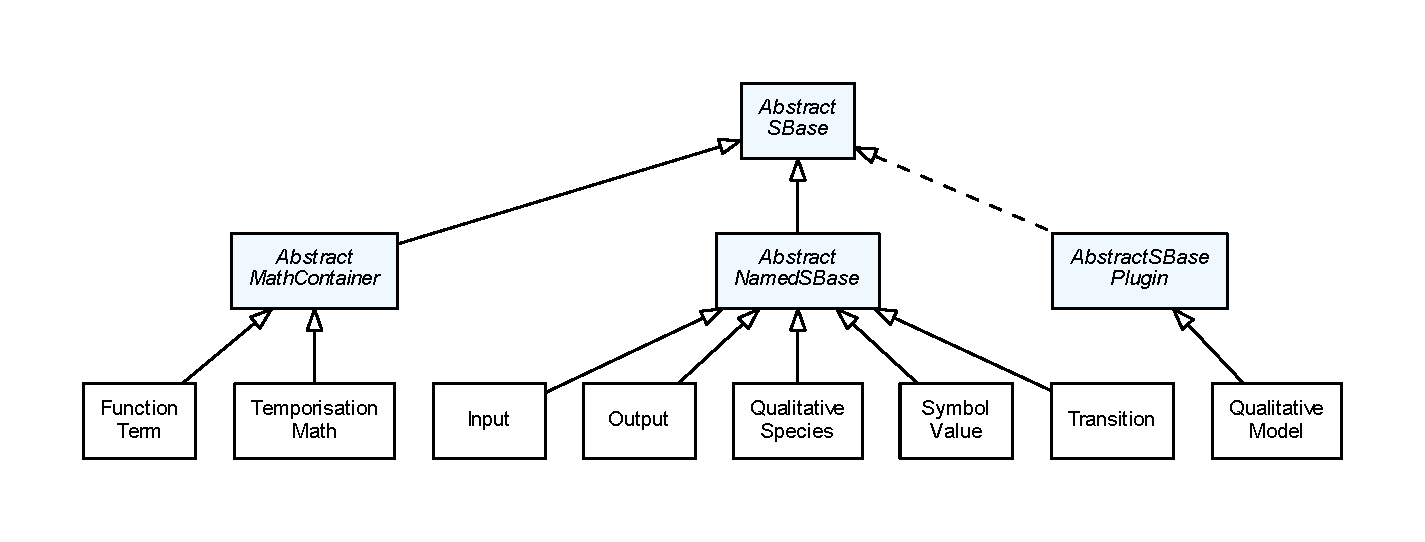
\includegraphics[width=\textwidth]{../../../extensions/qual/doc/img/type_hierarchy.pdf}
 \caption[Class diagram of the qualitative models extension]{Class diagram of the qualitative models extension. Qualitative Models package (\code{qual}, for short) allows species in a model to 
have non-quantitative or non-continuous concentrations \cite{Chaouiya2013}. 
This may manifest as Boolean or discrete values, and is primarily employed in 
modelling gene regulation, signalling pathways, and metabolic networks using 
logical/Boolean networks \cite{shmulevich2002} or Petri nets 
\cite{breitling2008}, which in turn, do not rely on traditional quantitative
coefficients to encode relationships between biochemical entities.}
 \label{fig:qual}
\end{figure}

\begin{figure}[hb]
 \centering
 \vspace*{2ex}
 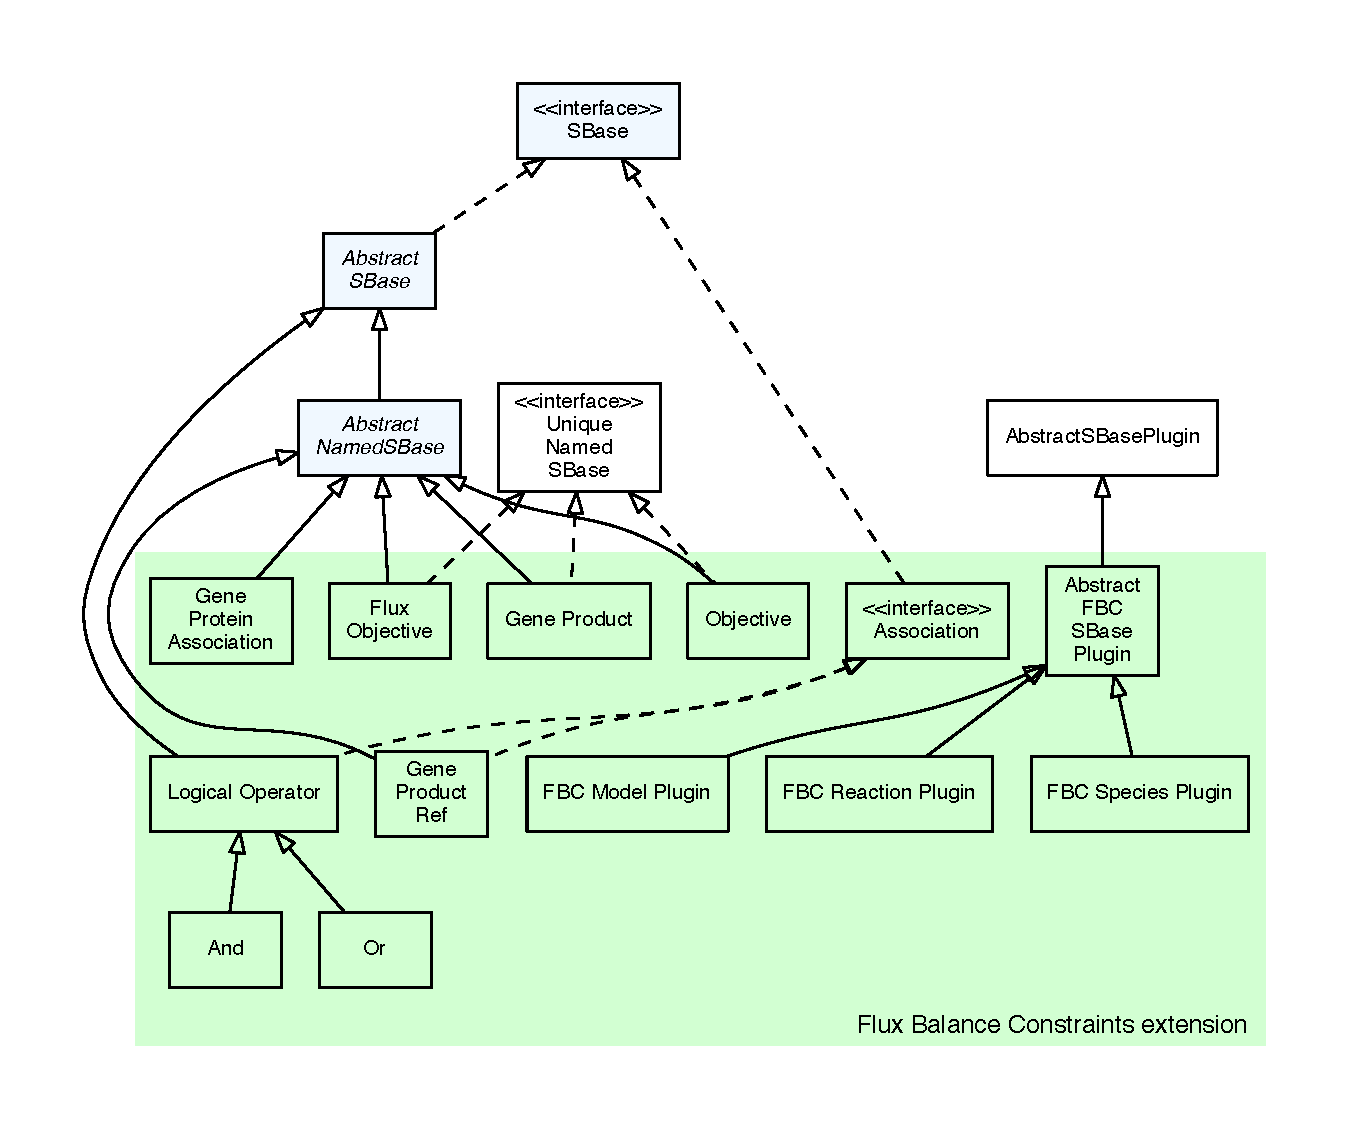
\includegraphics[width=\textwidth]{../../../extensions/fbc/doc/img/type_hierarchy.pdf}
 \caption[Class diagram of the flux balance constraints extension.]{Class diagram of the flux balance constraints extension. Constraints-based modelling \cite{lewis2012} utilizes a class of models in which
the canonical stoichiometric relations between reactions and metabolites are specified
as constraints for convex analysis and mathematical optimization. Although species,
reactions, and stoichiometry can be encoded using the SBML L3V1,
Flux Balance Constraints (\code{fbc}, \cite{olivier2013}) enable a constraints
based perspective. For example, the constraints based approach called
Flux Balance Analysis (FBA) often aims to find the maximum growth rate of the
cell given a set of uptake possibilities and the ratio of molecules needed
for cell growth. The mathematical formulation for this optimization problem
has variables of reaction fluxes and constraints of mass balances around the
metabolites and bounds on the variable reaction fluxes. Because this formulation is
underdetermined, an objective, usually one that maximizes a biomass function which
corresponds to growth rate, is supplied which optimizes the reaction fluxes. Therefore,
the \code{fbc} package extends the SBML Level 3 core to specifically encode for bounds on
fluxes, constraints, and objective functions, which facilitates a fluid interface to
existing constraints-based modelling software and optimization solvers.}
 \label{fig:fbc}
\end{figure}

\begin{figure}[hb]
 \centering
 \vspace*{2ex}
 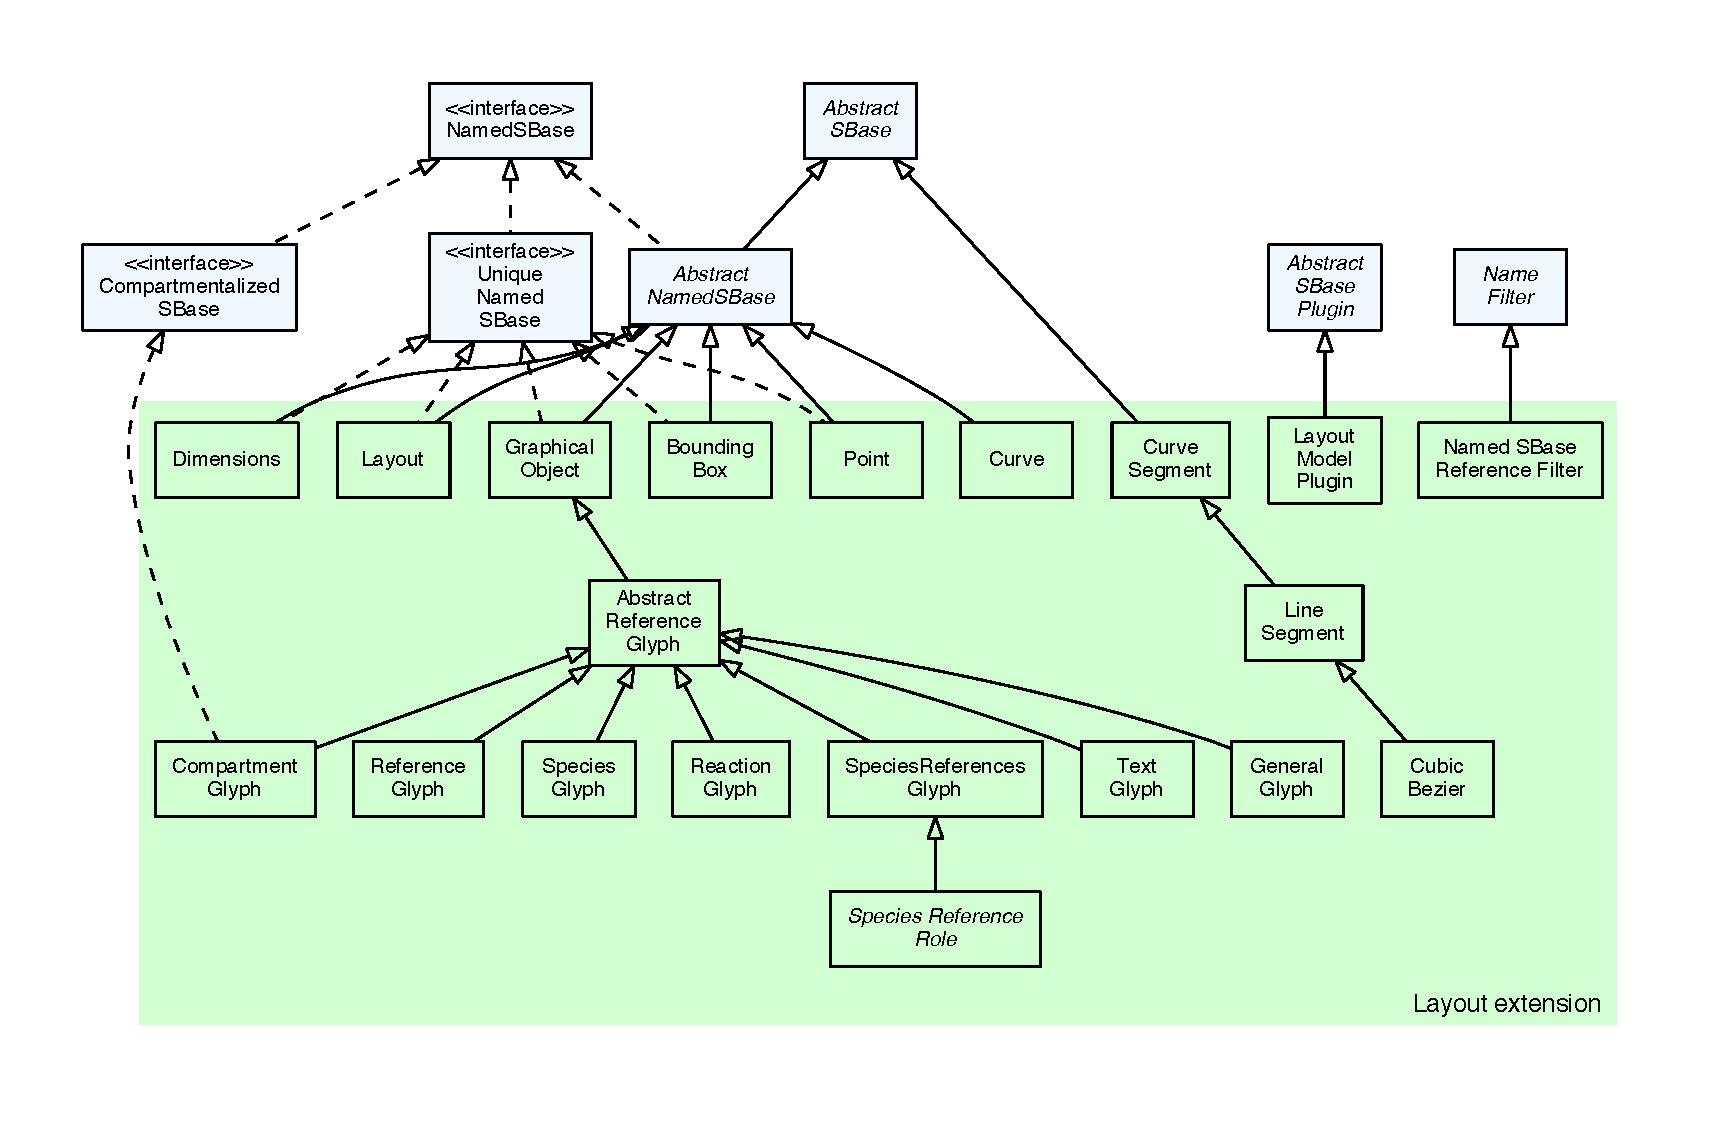
\includegraphics[width=\textwidth]{../../../extensions/layout/doc/img/type_hierarchy.pdf}
 \caption[Class diagram of the layout extension]{Class diagram of the layout extension. SBML encodes a core set of components (species, reactions) that make up
biochemical networks. The \code{layout} extension supports specifying graphical
information for these components. The structure for this extension mirrors 
the SBML Level 3 core hierarchy by introducing graphical object (\code{glyph})
counterparts to reactions and species. Different \code{glyph} types can optionally correspond
to elements in standard SBML, and there can be many \code{glyphs} for one element.
In addition, \code{layout} elements of non-standard model components can be specified
using the generic \code{GraphicalObject} class. Although this extension is powerful
enough to encode the position of all biochemically related graph components,
it should be noted that the scope of this package does not include rendering
of these components. This functionality is provided by the \code{Render} package.
Ultimately, the \code{layout} extension provides a common language that biochemical
graph editors and viewers can utilize to couple a model to a graph layout.}
 \label{fig:layout}
\end{figure}

\begin{figure}[hb]
 \centering
 \vspace*{2ex}
 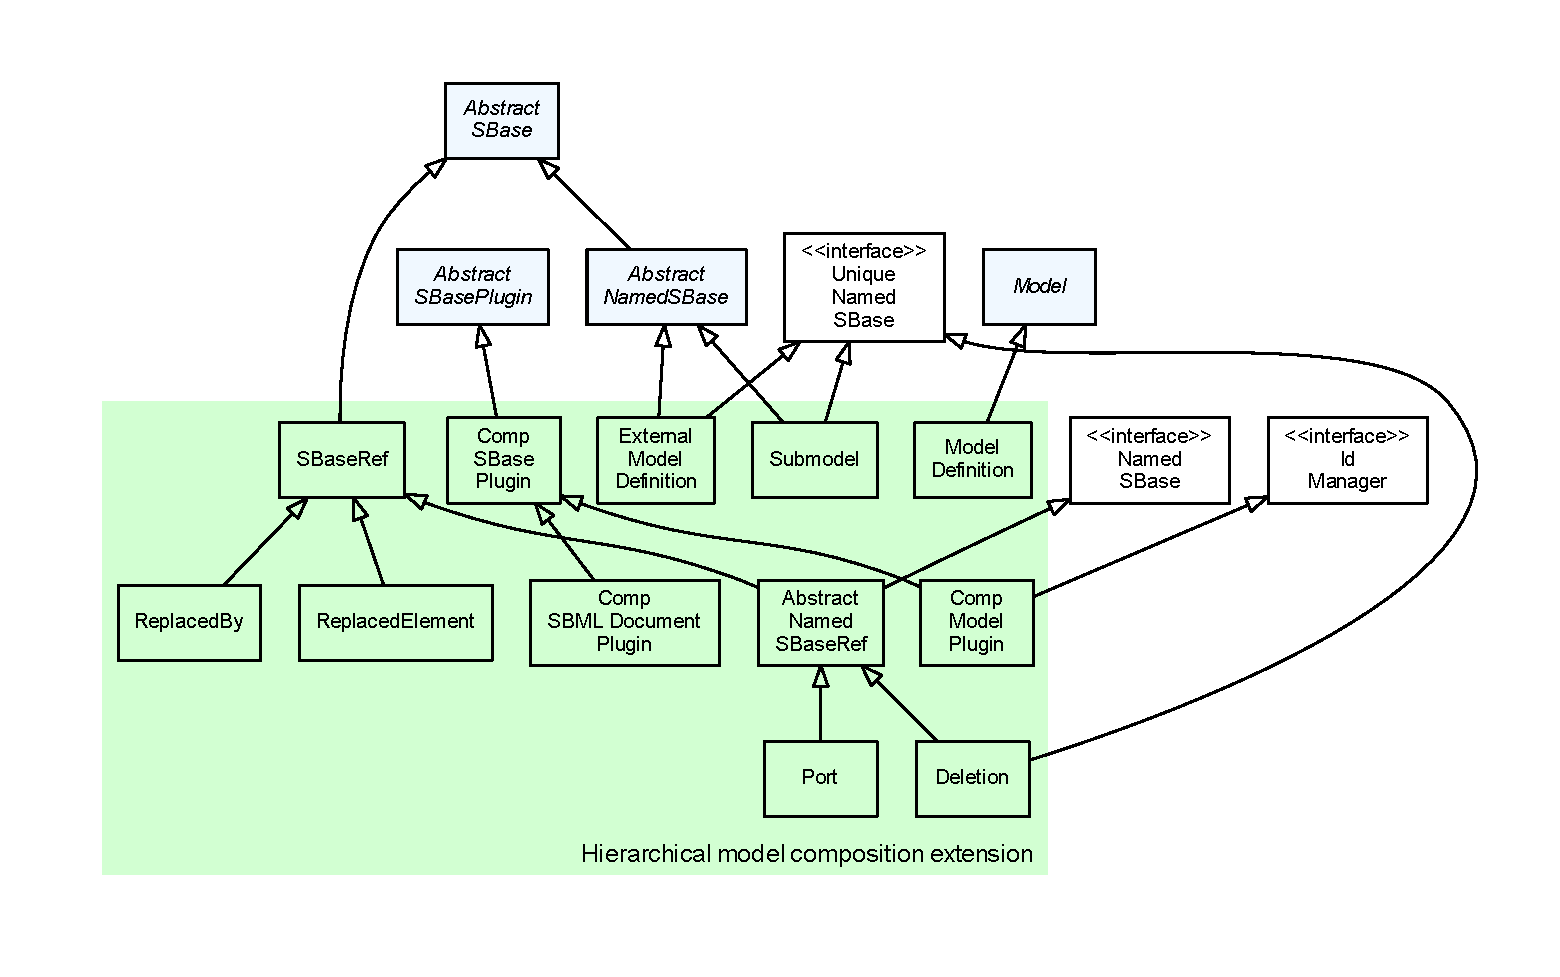
\includegraphics[width=\textwidth]{../../../extensions/comp/doc/img/type_hierarchy.pdf}
 \caption[Class diagram of the hierarchical model composition extension]{Class diagram of the hierarchical model composition extension. As the amount of information for biochemical networks increases, models tend to
increase in complexity as well. The Hierarchical Model Composition extension (\code{comp}; \cite{smith2010})
attempts to contextualize this complexity by providing a generic framework to encode
models as hierarchical entities in an SBML document. This functionality also allows
for storing multiple instances of a model within an enclosing model or document, which
can be used to build libraries of models within a document or to independently manage
different parts of a large model. Classes allow modellers to access elements within
sub-models and interface with other sub-models, and \code{comp} provides a standardized approach
to define sub-model differences with respect to parent or reference models. Overall, \code{comp}
is a powerful extension to the SBML Level 3 core that gives modellers and programmers
options to standardize the encoding of complex, modular modelling frameworks. 
}
 \label{fig:comp}
\end{figure}

\begin{figure}[hb]
 \centering
 \vspace*{2ex}
 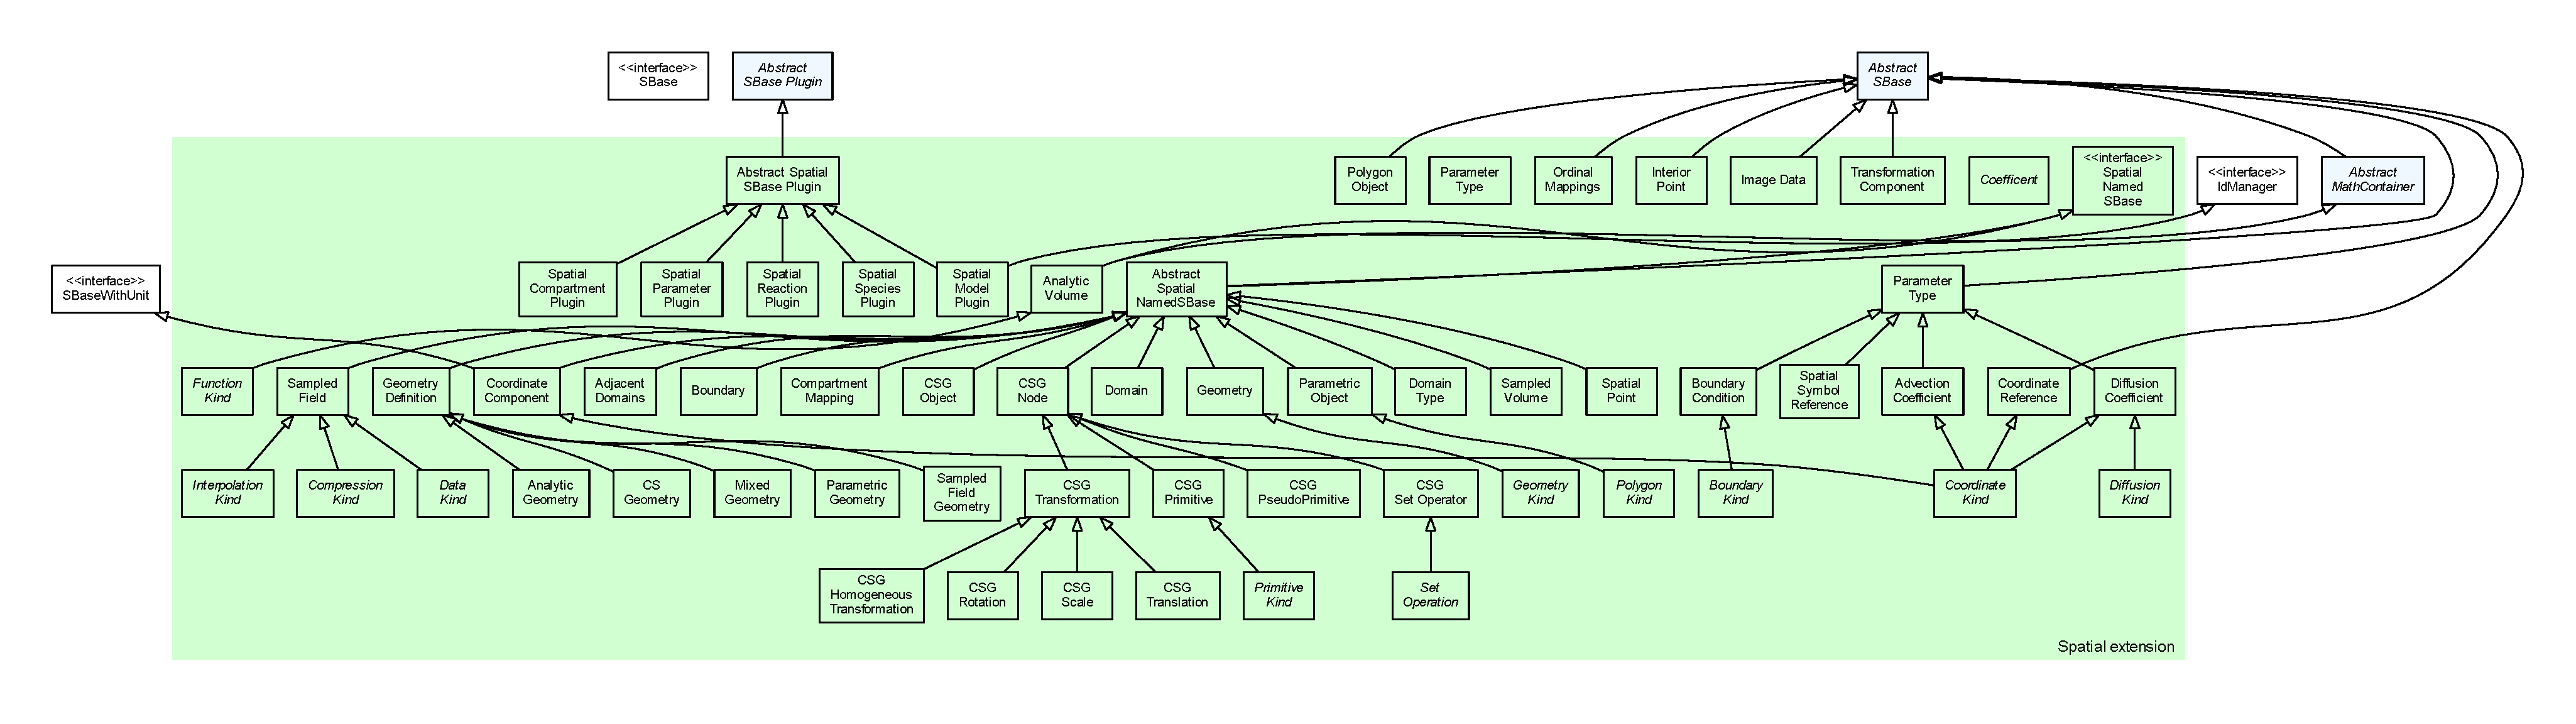
\includegraphics[width=\textwidth]{../../../extensions/spatial/doc/img/type_hierarchy.pdf}
 \caption[Class diagram of the spatial processes extension]{Class diagram of the spatial processes extension. The Spatial Processes extension (\code{spatial}, \cite{Schaff2014})
provides the ability to the SBML Level 3 core to specify subcellular,
geometric locations for components in biochemical
models. Although subcellular locations can be abstractly represented via
compartments in the SBML core specifications, \code{spatial} enables the encoding of
a cellular coordinate system which can describe non-uniform molecular distributions,
diffusive transport, and spatially localized reactions. The \code{Geometry} class holds
the spatial information and the extended \code{Species}, \code{Reaction}, \code{Compartment}, and
\code{Parameter} objects have mappings to the \code{spatial} objects that hold information on
molecular transport coefficients, geometric domains, and coordinates. \code{Spatial} is
therefore able to store the geometric information commonly used in spatial modelling
tools for the biochemical entities from standard SBML.}
 \label{fig:spatial}
\end{figure}

\begin{figure}[hb]
 \centering
 \vspace*{2ex}
 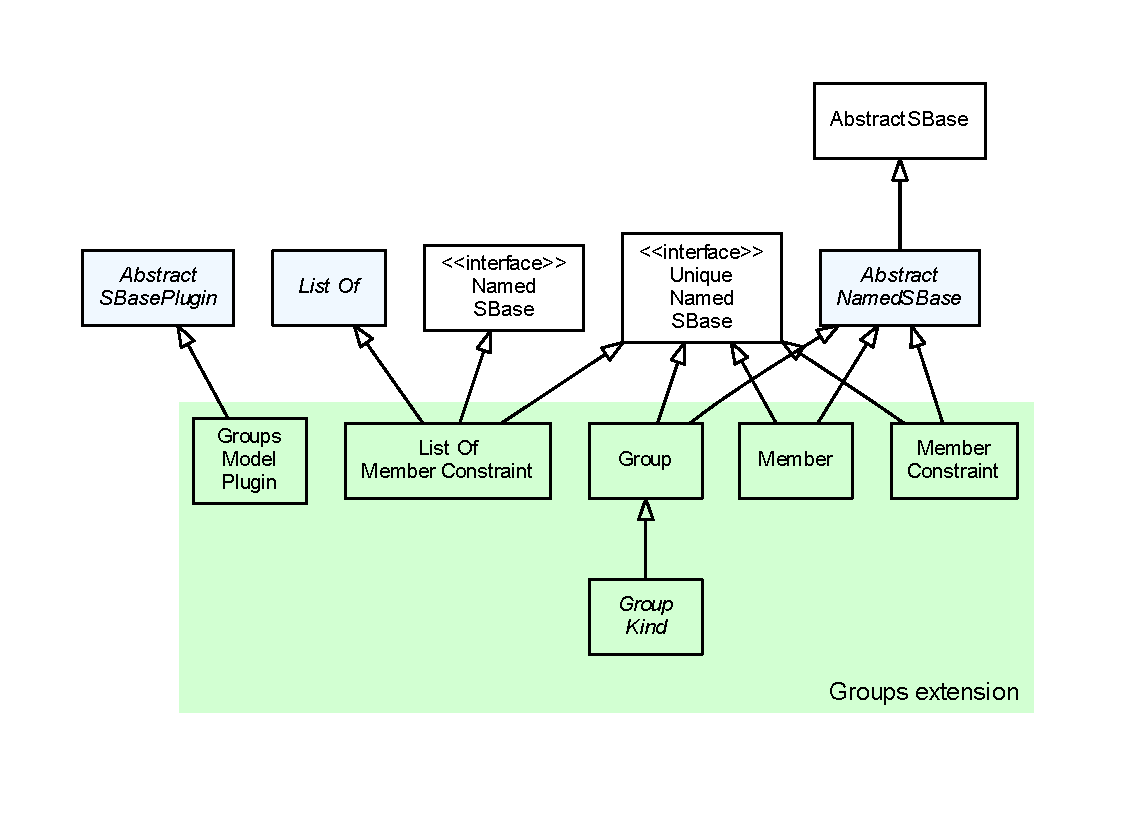
\includegraphics[width=\textwidth]{../../../extensions/groups/doc/img/type_hierarchy.pdf}
 \caption[Class diagram of the groups extension]{Class diagram of the groups extension. \code{Groups} is a simple extension that links together elements in an SBML model. Coupling
\code{groups} information with annotation and SBO terms \cite{Courtot2011a} 
contextualizes these sets of objects for properly conveying roles of groups 
for other programmers and modellers.}
 \label{fig:groups}
\end{figure}


\begin{figure}[hb]
 \centering
 \vspace*{2ex}
 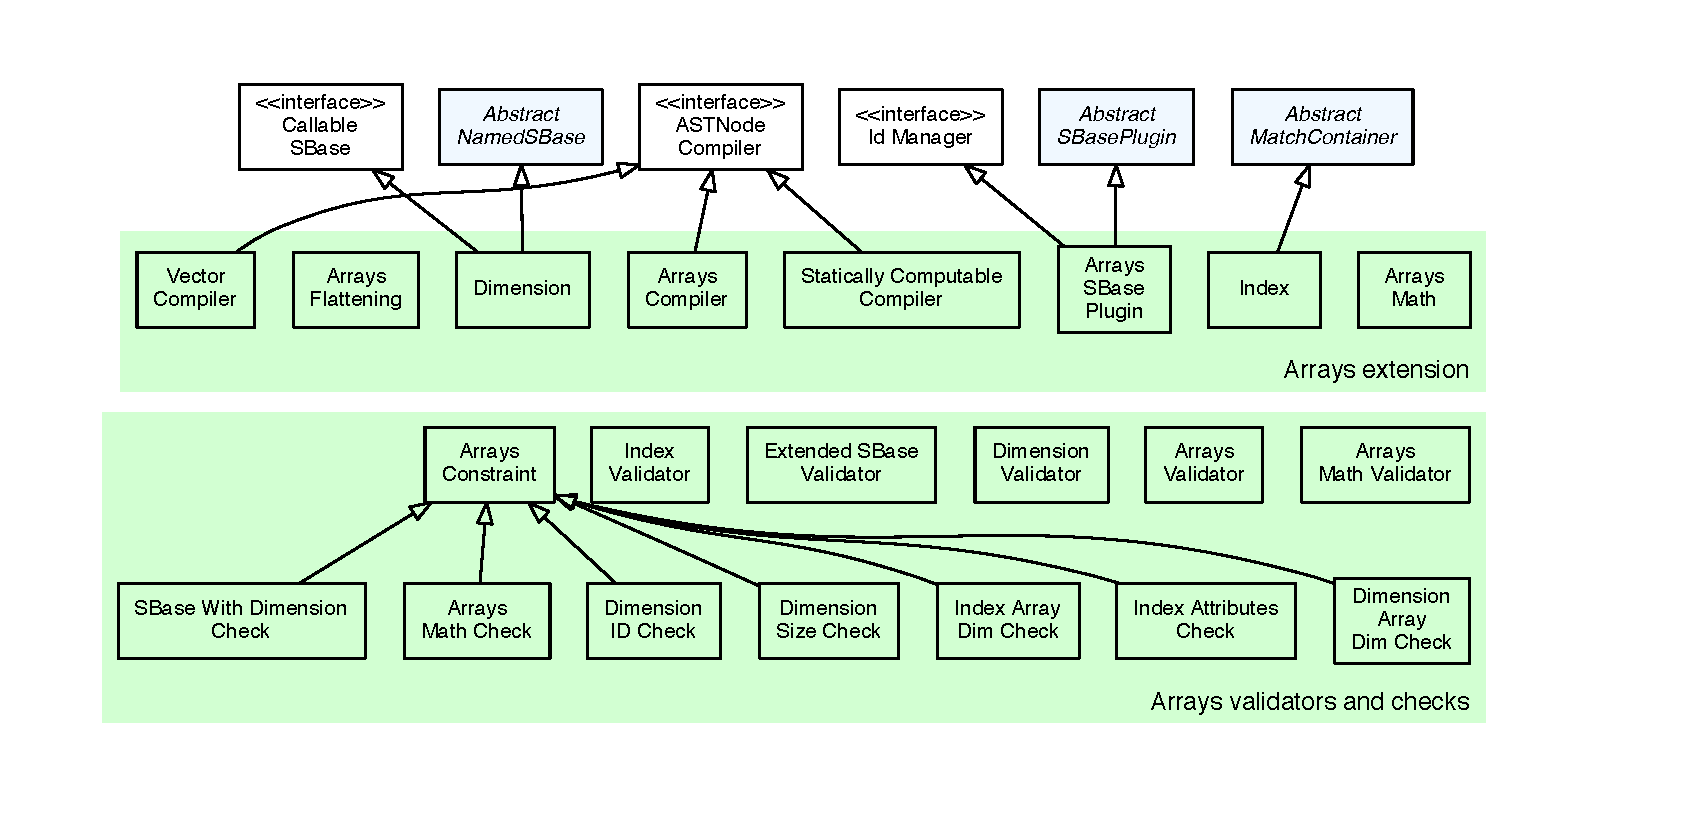
\includegraphics[width=\textwidth]{../../../extensions/arrays/doc/img/type_hierarchy.pdf}
 \caption[Class diagram of the arrays extension]{Class diagram of the arrays extension. Arrays (\code{arrays}, \cite{Watanabe2013}) extends SBML variables to include arrays of values,
thereby representing repeated or regular model structures more efficiently.
\code{Arrays} provides the ability to access sets of values with indices instead of explicit
declaration and creation of sub-data objects.}
 \label{fig:arrays}
\end{figure}


\begin{figure}[hb]
 \centering
 \vspace*{2ex}
 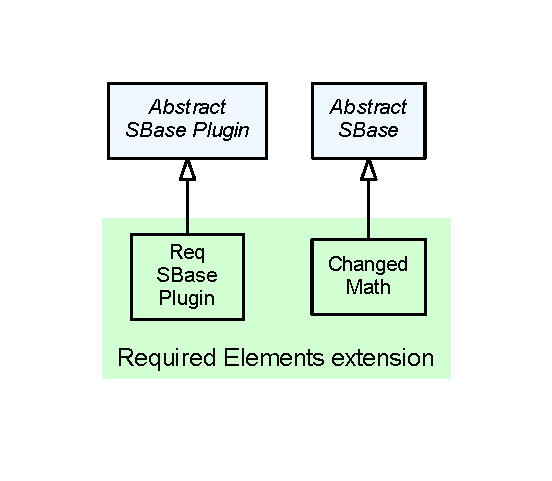
\includegraphics[width=.5\textwidth]{../../../extensions/req/doc/img/type_hierarchy.pdf}
 \caption[Class diagram of the required elements extension]{Class diagram of the required elements extension. Required Elements (\code{req}, \cite{Smith2013}) allows a model to indicate which
components have had their mathematical meanings changed by (e.g.) the use of
another SBML package.}
 \label{fig:arrays}
\end{figure}


\begin{figure}[hb]
 \centering
 \vspace*{2ex}
 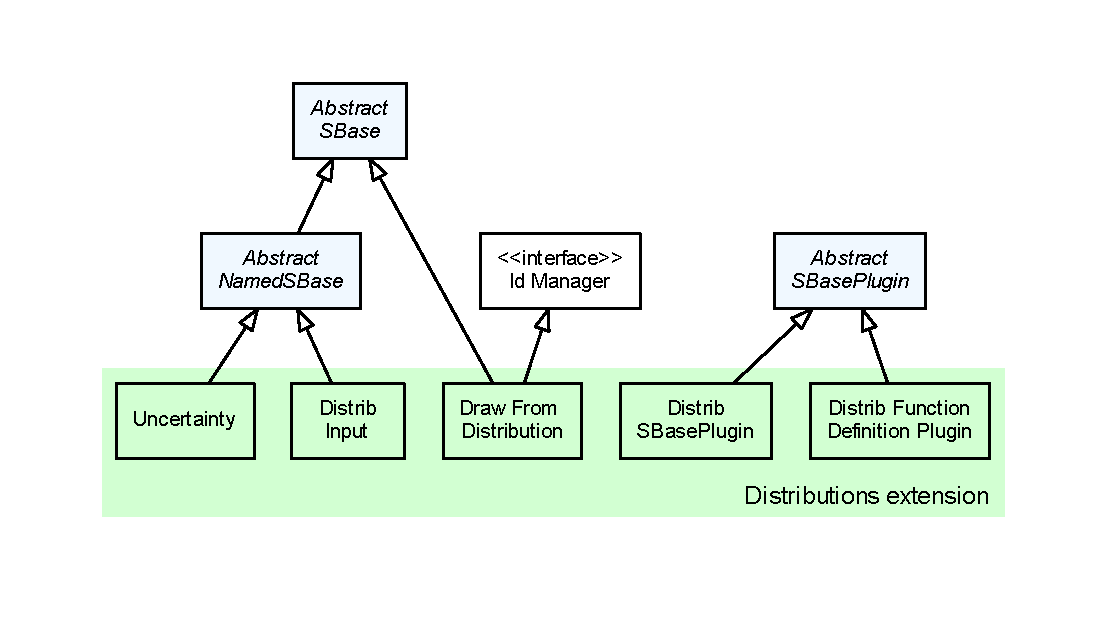
\includegraphics[width=\textwidth]{../../../extensions/distrib/doc/img/type_hierarchy.pdf}
 \caption[Class diagram of the distributions extension.]{ Class diagram of the distributions extension. Distributions 
 (\code{distrib}, \cite{Moodie2013}) encodes statistical distributions and their sampling.}
 \label{fig:distrib}
\end{figure}

\begin{figure}[hb]
 \centering
 \vspace*{2ex}
 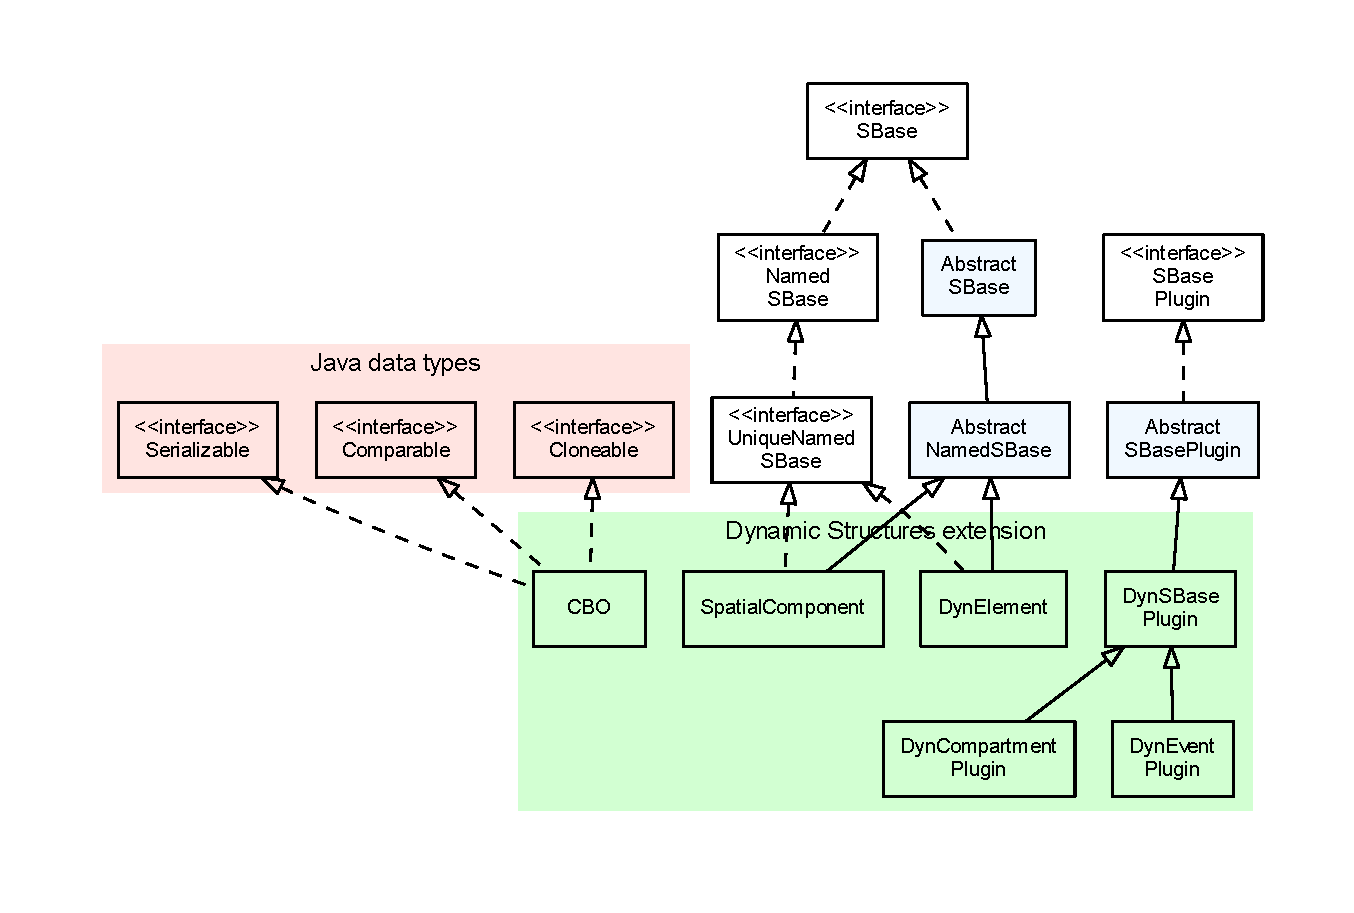
\includegraphics[width=\textwidth]{../../../extensions/dyn/doc/img/type_hierarchy.pdf}
 \caption[Class diagram of the dynamic structures extension]{Class diagram of the dynamic structures extension. Dynamic Structures (\code{dyn}, \cite{Gomez2014}), supports the definition of dynamical behaviors for model entities.
}
 \label{fig:dyn}
\end{figure}


\begin{figure}[hb]
 \centering
 \vspace*{2ex}
 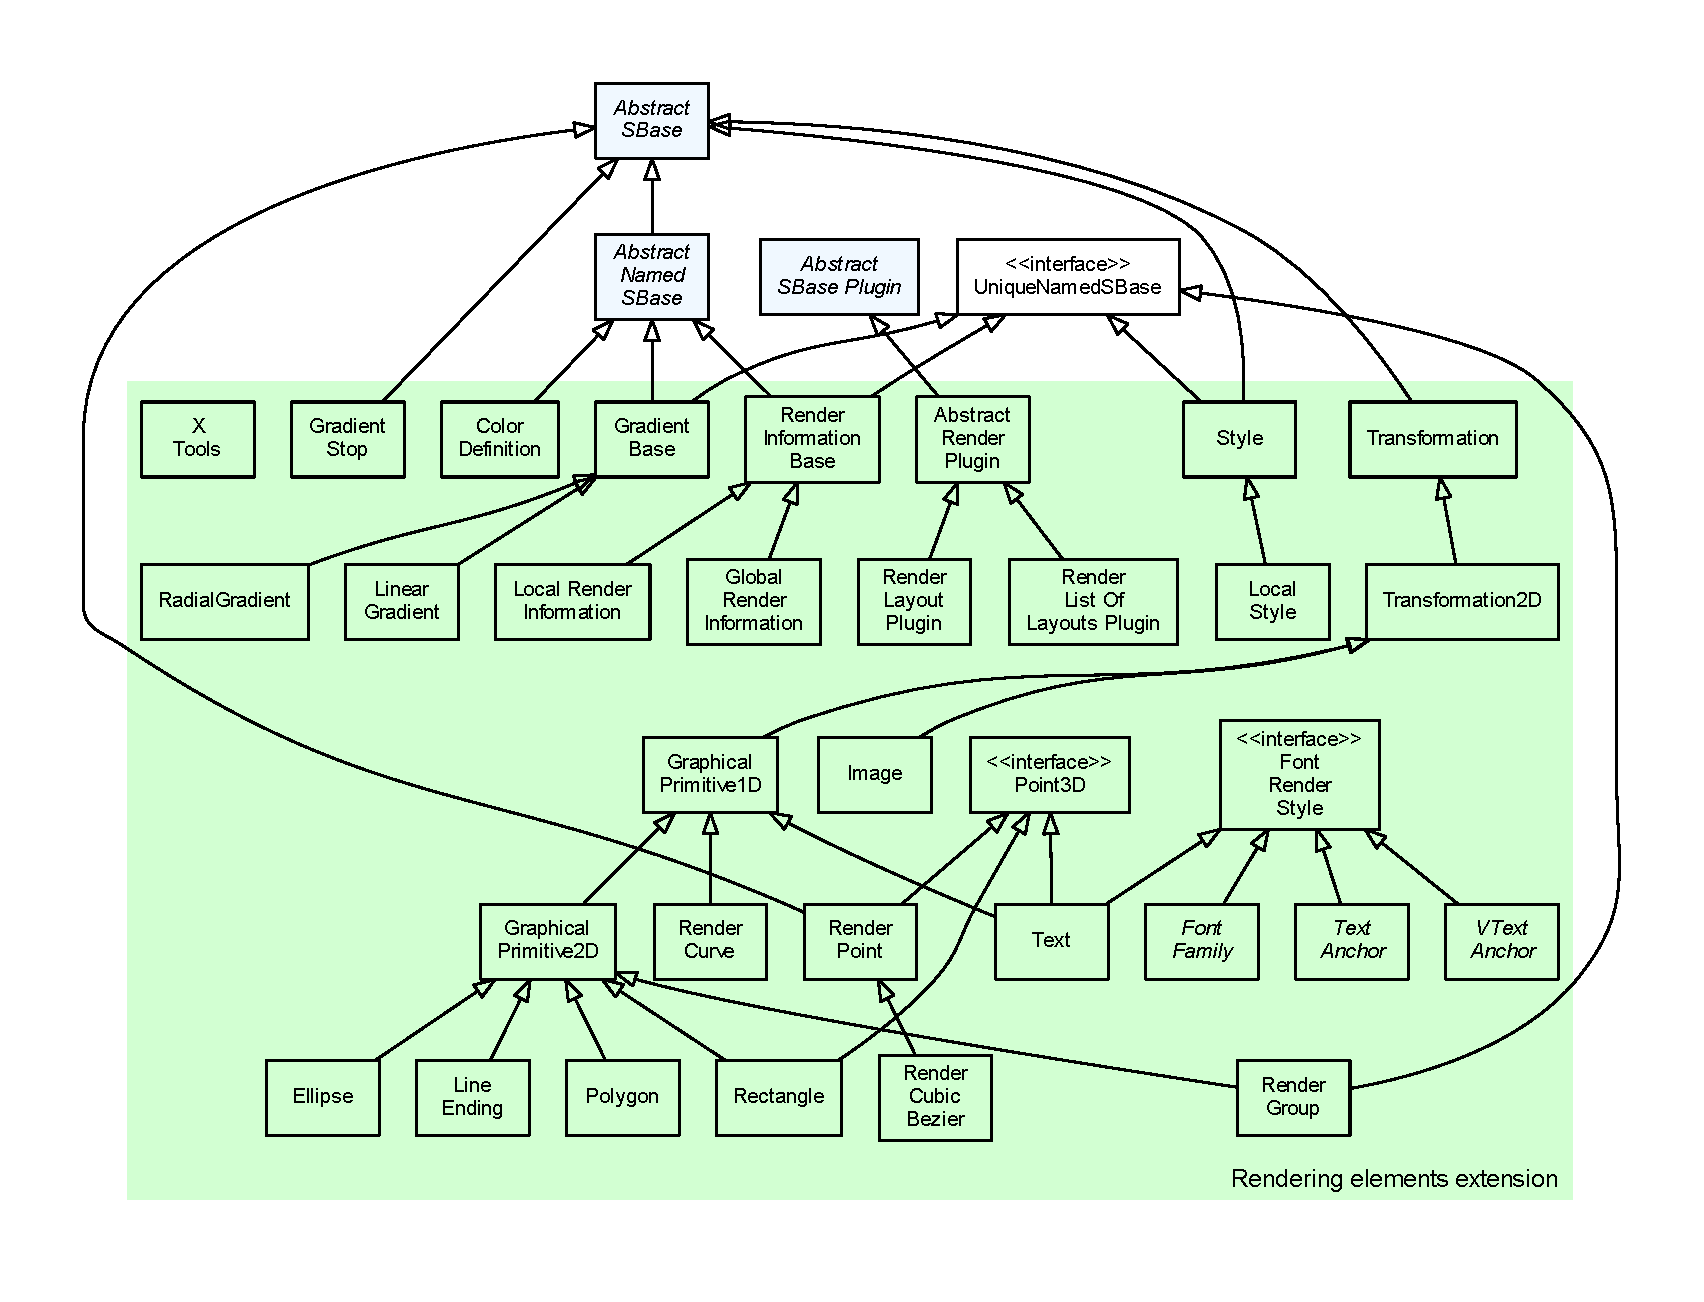
\includegraphics[width=\textwidth]{../../../extensions/render/doc/img/type_hierarchy.pdf}
 \caption[Class diagram of the rendering extension.]{Class diagram of the rendering extension. Rendering (\code{render}, \cite{gauges2006}) couples with \cite{Layout} to provide symbol and style information for network diagrams.}
 \label{fig:render}
\end{figure}





\chapter{Acknowledgments}
\label{chp:acknowledgements}

% -*- TeX-master: "User_guide"; fill-column: 75 -*-

The development and support of JSBML is a substantial undertaking and many
people have put in time and effort on this project.  The authors especially
thank the following individuals for their many contributions to JSBML:
Meike Aichele, Sebastian Fr\"ohlich, Roland Keller, Sarah Rachel M\"uller
vom Hagen, Alexander Peltzer, and Simon Sch\"afer (in alphabetical order).

The development of JSBML is currently funded by the following
organizations:

\begin{itemize}

\item The National Institute of General Medical Sciences (USA) via grant
number R01~GM070923, 

\item The EMBL European Bioinformatics Institute (Germany and UK), and

\item The Federal Ministry of Education and Research (BMBF, Germany) via grant numbers 0315756 and 0315384C for the \emph{Virtual Liver Network} and the MedSys (Medical Systems Biology) project \emph{Spher4Sys}.

\end{itemize}

Last but not least, JSBML is an open-source project, and we thank others
who have helped in its progress, in the form of comments, bug reports, bug
fixes, and other contributions.

Other interested people are welcome to join the team and to contribute to
the project.  The JSBML Team also explicitely encourages students who would
like to participate in a large software project, to ask for current
JSBML subprojects that are in need of doing.


% -----------------------------------------------------------------------------
% Appendix
% -----------------------------------------------------------------------------

\appendix

\chapter{Frequently Asked Questions (FAQ)}
\label{chp:faq}

For questions regarding SBML, please see the SBML FAQ at
\url{http://sbml.org/Documents/FAQ}.
\begin{description}
\item[Why does the class \texttt{LocalParameter} not inherit from
\texttt{Parameter}?]
\index{parameter!\texttt{LocalParameter}}
\index{parameter!\texttt{Parameter}}
The reason is the Boolean
\index{Boolean}
attribute \texttt{constant}, which is present in
\index{constant}
\index{parameter!\texttt{constant}}
\texttt{Parameter} and can be set to \texttt{false}. A parameter in the meaning
of SBML is not a constant, it might be some system variable
\index{JSBML!variable@\texttt{Variable}}
and can therefore be the subject of \texttt{Rule}s,
\index{rule}
\texttt{Event}s\index{event!\texttt{Event}}, \texttt{InitialAssignment}s
\index{InitialAssignment@\texttt{InitialAssignment}}
and so on, i.e., all instances of \texttt{Assignment},
\index{JSBML!assignment@\texttt{Assignment}}
whereas a \texttt{LocalParameter} is defined as a constant quantity that never
changes its value during the evaluation of a model\index{model}. It would
therefore only be possible to let \texttt{Parameter} inherit from
\texttt{LocalParameter} but this could lead to a semantic misinterpretation.


\item[Does JSBML depend on SWING or any particular graphical user interface
implementation?]
Although all classes in JSBML implement the \texttt{TreeNode} interface, which
is located in the package \texttt{javax.swing.tree}, all classes in JSBML are
entirely independent from any graphical user interface, such as the SWING
implementation. When loading the \texttt{TreeNode} interface, no other class
from SWING will be initialized or loaded; hence JSBML can also be used on
computers that do not provide any graphical system without the necessity of
catching a \texttt{HeadlessException}. The \texttt{TreeNode} interface only
defines methods and properties that all recursive tree data structures have to
implement anyway. Letting JSBML classes extend this interface makes JSBML
compatible with many other Java classes and methods that make use of the
standard \texttt{TreeNode} interface, hence ensuring a high compatibility with
other Java libraries. Since the SWING package belongs to the standard
Java\texttrademark{} distribution, it is ensured that the \texttt{TreeNode}
interface can always be localized by the Java Virtual Machine,
independent from the specific hardware or system.

\item[Does the usuage of the the \texttt{java.beens} package for the
\texttt{TreeNodeChangeListener} lead to an incompatibility with light-weight
Java installations?]
With the \texttt{java.beens} package being part of the standard Java
distribution, such an incompatibility will not occur. Extending existing
standard Java classes leads to a higher compatibility with other libraries and
should therefore be the preferred way to go in the development of JSBML.
\end{description}


\chapter{Open tasks in JSBML development}
\label{chp:open-tasks}

\begin{itemize}
\item JSBML does not yet provide a complete validator for SBML.
\item The support for SBML Level 3\index{SBML!Level~3} should be completed, particularly extension packages.\index{SBML!extension packages}
\item The \texttt{toSBML()}\index{SBase@\texttt{SBase}!\texttt{toSBML()}}
methods in \texttt{SBase} are still missing.
\item Constructors and methods with namespaces are not yet provided.
\item The libSBML compatibility module\index{libSBML!compatibility module} need
to be implemented.
\end{itemize}



% -----------------------------------------------------------------------------
% References
% -----------------------------------------------------------------------------

\clearpage

\thispagestyle{plain}
\pagestyle{plain}
\bibliography{../common/tex/literature}

% -----------------------------------------------------------------------------
% Index
% -----------------------------------------------------------------------------

\setindexprenote{\vspace*{0.1ex}}
\printindex


\end{document}


%%% Local Variables: 
%%% fill-column: 75
%%% End: 
